% !TeX spellcheck = en_GB
%%%%%%%%%%%%%%%%%%%%%%%%%%%%%%%%%%%%%%%%%%
%                                        %
%    Engineer thesis LaTeX template      % 
%  compliant with the SZJK regulations   %
%                                        %
%%%%%%%%%%%%%%%%%%%%%%%%%%%%%%%%%%%%%%%%%%
%                                        %
%  (c) Krzysztof Simiński, 2018-2023     %
%                                        %
%%%%%%%%%%%%%%%%%%%%%%%%%%%%%%%%%%%%%%%%%%
%                                        %
% The latest version of the templates is %
% available at                           %
% github.com/ksiminski/polsl-aei-theses  %
%                                        %
%%%%%%%%%%%%%%%%%%%%%%%%%%%%%%%%%%%%%%%%%%
%
%
% This LaTeX project formats the final thesis 
% with compliance to the SZJK regulations. 
% Please to not change formatting (fonts, margins,
% bolds, italics, etc).
%
% You can compile the project in several ways.
%
% 1. pdfLaTeX compilation
% 
% pdflatex main
% bibtex   main
% pdflatex main
% pdflatex main
%
%
% 2. XeLaTeX compilation
%
% Compilation with the XeLaTeX engine inserts Calibri font
% in the title page. Of course the font has to be installed.
% 
% xelatex main
% bibtex  main
% xelatex main
% xelatex main
%
%
%%%%%%%%%%%%%%%%%%%%%%%%%%%%%%%%%%%%%%%%%%%%%%%%%%%%%%%%%%%%%%
% If you have any questions, remarks, just send me an email: %
%            krzysztof.siminski(at)polsl.pl               %
%%%%%%%%%%%%%%%%%%%%%%%%%%%%%%%%%%%%%%%%%%%%%%%%%%%%%%%%%%%%%%

% We would like to improve the LaTeX templates 
% of final theses. By answering the questions 
% in the survey whose address your can find below 
% you help us to do so. The survey is completely 
% anonimous. Thank you!
%
% https://docs.google.com/forms/d/e/1FAIpQLScyllVxNKzKFHfILDfdbwC-jvT8YL0RSTFs-s27UGw9CKn-fQ/viewform?usp=sf_link
%
%%%%%%%%%%%%%%%%%%%%%%%%%%%%%%%%%%%%%%%%%%%%%%%%%%%%%%%%%%%%%%%%%%%%%%%%%

%%%%%%%%%%%%%%%%%%%%%%%%%%%%%%%%%%%%%%%%%%%%%%%
%                                             %
% CUSTOMISATION OF THE THESIS                 %
%                                             %
%%%%%%%%%%%%%%%%%%%%%%%%%%%%%%%%%%%%%%%%%%%%%%%

% Please customise your thesis with the macros below.

% TODO
\newcommand{\Firstnames}{First Names}
\newcommand{\Surname}{Surname}
\newcommand{\Supervisor}{$\langle$title first name surname$\rangle$}  % supervisor (remove $\langle$ and $\rangle)
\newcommand{\Title}{Thesis title in English}
\newcommand{\TitleAlt}{Thesis title in Polish}
\newcommand{\Program}{Control, Electronic, and Information Engineering} 
\newcommand{\Specialisation}{Informatics}
\newcommand{\Id}{$\langle$your student id$\rangle$} %  (remove $\langle$ and $\rangle)
\newcommand{\Departament}{$\langle$departament name$\rangle$} % your supervisor's departament  (remove $\langle$ and $\rangle)


% If you have a consultant for your thesis, put their name below ...
\newcommand{\Consultant}{$\langle$title first name surname$\rangle$}  %  (remove $\langle$ and $\rangle)
% ... else leave the braces empty:
%\newcommand{\Consultant}{} % no consultant

% end of thesis customisation
%%%%%%%%%%%%%%%%%%%%%%%%%%%%%%%%%%%%%%%%%%

%%%%%%%%%%%%%%%%%%%%%%%%%%%%%%%%%%%%%%%%%%%%%%%
%                                             %
% END OF CUSTOMISATION                        %
%                                             %
%%%%%%%%%%%%%%%%%%%%%%%%%%%%%%%%%%%%%%%%%%%%%%%

%%%%%%%%%%%%%%%%%%%%%%%%%%%%%%%%%%%%%%%%  


%%%%%%%%%%%%%%%%%%%%%%%%%%%%%%%%%%%%%%%%%%%%%%%
%                                             %
%   PLEASE DO NOT MODIFY THE SETTINGS BELOW!  %
%                                             %
%%%%%%%%%%%%%%%%%%%%%%%%%%%%%%%%%%%%%%%%%%%%%%%



\documentclass[a4paper,twoside,12pt]{book}
\usepackage[utf8]{inputenc}                                      
\usepackage[T1]{fontenc}  
\usepackage{amsmath,amsfonts,amssymb,amsthm}
\usepackage[polish,british]{babel} 
\usepackage{indentfirst}



\usepackage{ifxetex}

\ifxetex
	\usepackage{fontspec}
	\defaultfontfeatures{Mapping=tex—text} % to support TeX conventions like ``——-''
	\usepackage{xunicode} % Unicode support for LaTeX character names (accents, European chars, etc)
	\usepackage{xltxtra} % Extra customizations for XeLaTeX
\else
	\usepackage{lmodern}
\fi



\usepackage[margin=2.5cm]{geometry}
\usepackage{graphicx} 
\usepackage{hyperref}
\usepackage{booktabs}
\usepackage{tikz}
\usepackage{pgfplots}
\usepackage{mathtools}
\usepackage{geometry}
\usepackage{subcaption}   % subfigures
\usepackage[page]{appendix} % toc,




\usepackage{csquotes}
\usepackage[natbib=true,backend=bibtex,maxbibnames=99]{biblatex}  % compilation of bibliography with BibTeX
%\usepackage[natbib=true,backend=biber,maxbibnames=99]{biblatex}  % compilation of bibliography with Biber
\bibliography{biblio/biblio}

\usepackage{ifmtarg}   % empty commands  

\usepackage{setspace}
\onehalfspacing


\frenchspacing



%%%% TODO LIST GENERATOR %%%%%%%%%

\usepackage{color}
\definecolor{brickred}      {cmyk}{0   , 0.89, 0.94, 0.28}

\makeatletter \newcommand \kslistofremarks{\section*{Remarks} \@starttoc{rks}}
  \newcommand\l@uwagas[2]
    {\par\noindent \textbf{#2:} %\parbox{10cm}
{#1}\par} \makeatother


\newcommand{\ksremark}[1]{%
{%\marginpar{\textdbend}
{\color{brickred}{[#1]}}}%
\addcontentsline{rks}{uwagas}{\protect{#1}}%
}










%%%%%%%%%%%%%% END OF TODO LIST GENERATOR %%%%%%%%%%%  

%%%%%%%%%%%% FANCY HEADERS %%%%%%%%%%%%%%%
% no capitalisation of headers
\usepackage{fancyhdr}
\pagestyle{fancy}
\fancyhf{}
\fancyhead[LO]{\nouppercase{\it\rightmark}}
\fancyhead[RE]{\nouppercase{\it\leftmark}}
\fancyhead[LE,RO]{\it\thepage}


\fancypagestyle{onlyPageNumbers}{%
   \fancyhf{} 
   \fancyhead[LE,RO]{\it\thepage}
}

\fancypagestyle{noNumbers}{%
   \fancyhf{} 
   \fancyhead[LE,RO]{}
}


\fancypagestyle{PageNumbersChapterTitles}{%
   \fancyhf{} 
   \fancyhead[LO]{\nouppercase{\Firstnames\ \Surname}}
   \fancyhead[RE]{\nouppercase{\leftmark}} 
   \fancyfoot[CE, CO]{\thepage}
}
 



%%%%%%%%%%%%%%%%%%%%%%%%%%%







\newcounter{pagesWithoutNumbers}

%%%%%%%%%%%%%%%%%%%%%%%%%%% 
\usepackage{xstring}
\usepackage{ifthen}
\newcommand{\printOpiekun}[1]{%		

    \StrLen{\Consultant}[\mystringlen]
    \ifthenelse{\mystringlen > 0}%
    {%
       {\large{\bfseries CONSULTANT}\par}
       
       {\large{\bfseries \Consultant}\par}
    }%
    {}
} 
%
%%%%%%%%%%%%%%%%%%%%%%%%%%%%%%%%%%%%%%%%%%%%%%
 
% Please do not modify the lines below!
\author{\Firstnames\ \Surname}
\newcommand{\Author}{\Firstnames\ \MakeUppercase{\Surname}}
\newcommand{\Type}{FINAL PROJECT}
\newcommand{\Faculty}{Faculty of Automatic Control, Electronics and Computer Science}
\newcommand{\Polsl}{Silesian University of Technology}
\newcommand{\Logo}{graf/politechnika_sl_logo_bw_pion_en.pdf}
\newcommand{\LeftId}{Student identification number}
\newcommand{\LeftProgram}{Programme}
\newcommand{\LeftSpecialisation}{Specialisation}
\newcommand{\LeftSUPERVISOR}{SUPERVISOR}
\newcommand{\LeftDEPARTMENT}{DEPARTMENT}
%%%%%%%%%%%%%%%%%%%%%%%%%%%%%%%%%%%%%%%%%%%%%%

%%%%%%%%%%%%%%%%%%%%%%%%%%%%%%%%%%%%%%%%%%%%%%%
%                                             %
% END OF SETTINGS                             %
%                                             %
%%%%%%%%%%%%%%%%%%%%%%%%%%%%%%%%%%%%%%%%%%%%%%%

 % Do not modify!


%%%%%%%%%%%%%%%%%%%%%%%%%%%%%%%%%%%%%%%%%%%%%%%
%                                             %
% MY PACKAGES, SETTINGS ETC.                  %
%                                             %
%%%%%%%%%%%%%%%%%%%%%%%%%%%%%%%%%%%%%%%%%%%%%%%

% Put your packages, macros, setting here.


 
%%%%%%%%%%%%%%%%%%%%%%%%%%%%%%%%%%%%%%%%%%%%%%%%%%%%%%%%%%%%%%%%%%%%%
% listings
% packages: listings or minted
% % % % % % % % % % % % % % % % % % % % % % % % % % % % % % % % % % % 

% package listings
\usepackage{listings}
\lstset{%
morekeywords={string,exception,std,vector},% add the keyword you need
language=C++,% C, Matlab, Python, SQL, TeX, XML, bash, ... – vide https://www.ctan.org/pkg/listings
commentstyle=\textit,%
identifierstyle=\textsf,%
keywordstyle=\sffamily\bfseries, %\texttt, %
%captionpos=b,%
tabsize=3,%
frame=lines,%
numbers=left,%
numberstyle=\tiny,%
numbersep=5pt,%
breaklines=true,%
%morekeywords={descriptor_gaussian,descriptor,partition,fcm_possibilistic,dataset,my_exception,exception,std,vector},%
escapeinside={@*}{*@},%
}

% % % % % % % % % % % % % % % % % % % % % % % % % % % % % % % % % % % 
% package minted
% \usepackage{minted}

% This package requires a special command line option in compilation
% pdflatex -shell-escape main.tex
% xelatex  -shell-escape main.tex

%%%%%%%%%%%%%%%%%%%%%%%%%%%%%%%%%%%%%%%%%%%%%%%%%%%%%%%%%%%%%%%%%%%%%



%%%%%%%%%%%%%%%%%%%%%%%%%%%%%%%%%%%%%%%%%%%%%%%
%                                             %
% END OF MY PACKAGES, SETTINGS ETC.           %
%                                             %
%%%%%%%%%%%%%%%%%%%%%%%%%%%%%%%%%%%%%%%%%%%%%%%

 % Put your settings, packages, macros here.
 
%%%%%%%%%%%%%%%%%%%%%%%%%%%%%%%%%%%%%%%%   


\begin{document}
%\kslistofremarks 


%%%%%%%%%%%%%%%%%%%%%%%%%%%%%%%%%%%%%%%%%%%%%%%
%                                             %
%    PLEASE DO NOT MODIFY THE TITLE PAGE!     %
%                                             %
%%%%%%%%%%%%%%%%%%%%%%%%%%%%%%%%%%%%%%%%%%%%%%%


%%%%%%%%%%%%%%%%%%  TITLE PAGE %%%%%%%%%%%%%%%%%%%
\pagestyle{empty}
{
	\newgeometry{top=1.5cm,%
	             bottom=2.5cm,%
	             left=3cm,
	             right=2.5cm}
 
	\ifxetex 
	  \begingroup
	  \setsansfont{Calibri}
	   
	\fi 
	 \sffamily
	\begin{center}
	\includegraphics[width=50mm]{\Logo}
	 
	
	{\Large\bfseries\Type\par}
	
	\vfill  \vfill  
			 
	{\large\Title\par}
	
	\vfill  
		
	{\large\bfseries\Author\par}
	
	{\normalsize\bfseries \LeftId: \Id}
	
	\vfill  		
 
	{\large{\bfseries \LeftProgram:} \Program\par} 
	
	{\large{\bfseries \LeftSpecialisation:} \Specialisation\par} 
	 		
	\vfill  \vfill 	\vfill 	\vfill 	\vfill 	\vfill 	\vfill  
	 
	{\large{\bfseries \LeftSUPERVISOR}\par}
	
	{\large{\bfseries \Supervisor}\par}
				
	{\large{\bfseries \LeftDEPARTMENT\ \Departament} \par}
		
	{\large{\bfseries \Faculty}\par}
		
	\vfill  \vfill  

    	
    \printOpiekun{\Consultant}
    
	\vfill  \vfill  
		
    {\large\bfseries  Gliwice \the\year}

   \end{center}	
       \ifxetex 
       	  \endgroup
       \fi
	\restoregeometry
}
  
  % Please to not modify the titlepage.tex file!

\cleardoublepage
 
\rmfamily\normalfont
\pagestyle{empty}

  
%%% Let's start the thesis %%%%

% TODO
\subsubsection*{Thesis title} \Title

\subsubsection*{Abstract}  
(Thesis abstract – to be copied into an appropriate field during an electronic submission – in English.)

\subsubsection*{Keywords} 
(2-5 keywords, separated with commas)

\subsubsection*{Tytuł pracy} 
\begin{otherlanguage}{polish}
\TitleAlt
\end{otherlanguage}

\subsubsection*{Streszczenie} 
\begin{otherlanguage}{polish}
(Thesis abstract – to be copied into an appropriate field during an electronic submission – in Polish.)
\end{otherlanguage}
\subsubsection*{Słowa kluczowe}  
\begin{otherlanguage}{polish}
(2-5 keywords, separated by commas, in Polish)
\end{otherlanguage}

 % editorials


%%%%%%%%%%%%%%%%%% Table of contents %%%%%%%%%%%%%%%%%%%%%%
%\pagenumbering{Roman}
\thispagestyle{empty}
\tableofcontents
\thispagestyle{empty}

%%%%%%%%%%%%%%%%%%%%%%%%%%%%%%%%%%%%%%%%%%%%%%%%%%%%%
\setcounter{pagesWithoutNumbers}{\value{page}}
\mainmatter
\pagestyle{empty}
 
\cleardoublepage

\pagestyle{PageNumbersChapterTitles}

%%%%%%%%%%%%%% body of the thesis %%%%%%%%%%%%%%%%%

% TODO
\chapter{Introduction}

    Recently, there has been significant progress in terms of Artificial Intelligence (later called AI) and Machine Learning (later called ML). Projects that in the past could barely recognize some simple objects or try to recognize some patterns are now surpassed by programs like advanced chat bots that can talk about literally anything or AI’s that can create very realistic art. Many famous personas like Elon Musk or Bill Gates start to recognize the potential of AI. 
    As this field is rapidly growing it appears to be both reasonable and demanded to perform research in this area. 

% TODO
\chapter{[Problem analysis]}

\section*{What is AI and what can it be used for}
As the Cambridge Dictionary states, Artificial Intelligence is “the study of how to produce machines that have some of the qualities that the human mind has, such as the ability to understand language, recognize pictures, solve problems, and learn”. It can be concluded that Artificial Intelligence is a field of science whose goal is to replace the work of humans with machines.
AI is used for a wide variety of tasks and applications. Some examples include:
\begin{itemize}
    \item Image and speech recognition: AI algorithms can be trained to identify objects, people, or words in images or audio recordings.
    \item Language understanding: AI can be used to interpret and respond to natural language inputs, such as in virtual assistants or chatbots.
    \item Predictive analytics: AI can be used to analyze large data sets and make predictions about future events or trends.
    \item Robotics: AI controls and navigates robots, allowing them to perform tasks such as assembly line work or search-and-rescue operations.
    \item Self-driving cars: AI is used to interpret sensor data and decide how to control the car.
    \item Healthcare: AI can be used to analyze medical images, identify potential health risks, and assist doctors in making diagnoses.
    \item Fraud detection: AI can be used to identify suspicious patterns of behavior in financial transactions.
\end{itemize} 
These are just a few examples of the many ways AI is being used today, and as the technology continues to advance, it is likely to be used in an even wider range of applications in the future.

\section*{AI in stock prediction}
Since the beginning of Artificial Intelligence, people have wanted to use it for profit. The concept of a program that would be able to predict the future of the stock market is an idea that inspires many engineers to act. This is an unachievable goal, but AI is constantly evolving thanks to this challenge.

Predicting stock prices is a challenging task that has been the subject of much research in AI and machine learning. Various neural network architectures have been used for this task, and the choice of architecture will depend on the specific characteristics of the data and the problem at hand.
Some popular architectures that have been used for stock price prediction include:
\begin{itemize}
    \item Recurrent Neural Networks (RNNs): RNNs are particularly well-suited to sequential data, such as time series data, and have been used to predict stock prices by analyzing historical price and trading volume data.
    \item Long Short-Term Memory (LSTM) networks: LSTMs are a type of RNN that are able to maintain a long-term memory of the inputs it has seen and has been used to predict stock prices by analyzing historical price data.
    \item Convolutional Neural Networks (CNNs): CNNs are a type of neural network that are particularly well-suited to image and video data and have been used to predict stock prices by analyzing images of stock charts.
    \item Gated Recurrent Units (GRUs): Similar to LSTMs but with less computational complexity.
\end{itemize} 
It is worth noting that stock price prediction is a complex problem, and only some models would work best for some scenarios. Many other variables, such as news, announcements, market sentiments, and trends, also need to be taken into account and can be incorporated into the model using techniques like Sentiment Analysis and Named Entity Recognition.
It is also important to mention that stock prices are highly dynamic and non-linear, making it difficult to predict with high accuracy, and multiple models with different architectures may need to be combined to produce an accurate prediction.
\par
For this project, LSTM model have been chosen to predict the stock prices. 
One of the main reasons why LSTMs may be well-suited for stock price prediction is their ability to maintain a long-term memory of the inputs they have seen. Stock prices are a type of time series data, which means that the current price of a stock is likely to be influenced by a long sequence of previous prices and other related financial data, such as trading volume and market sentiment. Because LSTMs can maintain a long-term memory of the inputs they have seen, they can understand patterns or dependencies in the data that may span multiple time steps, making them well-suited to analyze historical price data and make predictions about future price movements.
Another reason LSTMs may be well-suited for stock price prediction is that they can handle input data with high dimensionality and noise. Stock prices are influenced by various factors, such as economic indicators, company news, and global events, which can be challenging to quantify or predict. LSTMs are able to handle input data with high dimensionality and high noise, making them well-suited to analyze a wide range of financial data and make predictions about future price movements.
Stock price prediction is a complicated problem and no single model would work best for every scenario. LSTM might work well on one dataset and not on another. Also, LSTMs alone might not be enough to accurately predict stock prices, and other techniques such as Sentiment Analysis and Named Entity Recognition, as well as other variables such as news, announcements, market sentiments and trends, may need to be taken into account and can be incorporated into the model.
\par
LSTM stands for Long Short-Term Memory. It is a type of Recurrent Neural Network (RNN) architecture that is used to process sequential data, such as time series or natural language.
An RNN processes input data one step at a time, maintaining an internal "memory" of the inputs it has seen. This allows the network to understand patterns or dependencies in the data that may span multiple time steps. However, the simple RNN architecture has a problem known as the "vanishing gradients" problem, where the gradients of the error concerning the parameters of the network become very small as they are backpropagated through multiple time steps.
By introducing a number of "gates" that regulate the movement of data into and out of the network's memory, LSTM finds a solution to this issue. These gates can be thought of as "switches" that turn the flow of information on and off, allowing the network to maintain a much longer-term memory of the inputs it has seen.
The LSTM architecture is used in various sequential data processing tasks, such as natural language processing, speech recognition, and time series prediction. LSTM is particularly well-suited to tasks where the output depends on a long sequence of prior inputs, such as in natural language processing or stock price prediction, as the output depends on many data

\section*{Prediction of the stock market}
Stock prices can be predicted using a combination of methods, including technical analysis, fundamental analysis, quantitative analysis, and news analysis.

\begin{itemize}
    \item Technical analysis: This method involves analyzing charts and historical data to identify patterns and trends that can indicate future stock price movements. Technical analysts look at factors such as support and resistance levels, moving averages, and trading volume to make predictions about future price movements.
    \item Fundamental analysis: This method involves analyzing a company's financial and economic fundamentals, such as earnings, revenue, and debt, to determine its intrinsic value and potential for future growth. Fundamental analysts look at a company's financial statements and other financial metrics to predict its future performance and stock price.
    \item Quantitative analysis: This method involves using mathematical models and algorithms to analyze financial data and make predictions about future stock prices. Quantitative analysts use statistical methods and machine learning techniques to analyze large amounts of data and make predictions about future stock prices.
    \item News analysis: This method involves analyzing news and events that may impact a company's stock price, such as changes in management, mergers, and acquisitions, or regulatory developments.
    \item It is important to note that no method is perfect, and past performance does not guarantee future results. Additionally, stock prices can be affected by many factors, including macroeconomic conditions, geopolitical events, and investor sentiment, which can be challenging to predict.
\end{itemize} 

Mathematical formulae  
\begin{align}
y = \frac{\partial x}{\partial t}
\end{align}
and single math symbols $x$ and $y$ are typeset in the mathematical mode.

  

% TODO
\chapter{Requirements and tools}

\begin{itemize}
\item functional and nonfunctional requirements
\item use cases (UML diagrams)
\item description of tools
\item methodology of design and implementation
\end{itemize} 

\section{Functional requirements}
Functional Requirements for a Stock Price Prediction System
\begin{itemize}
    \item Data Input: The system must be able to accept and process historical stock prices; depending on the choice of the user, it should be able to read open price, close price, highest price, lowest price, and average price.
    \item Data Preprocessing: The system must be able to clean, format, and prepare the data for analysis. It should scale the data appropriately to make it easier to fetch it into the neural network.
    \item Model Training: The system must be able to train an LSTM neural network model using historical data.
    \item Model Evaluation: The system must be able to evaluate the performance of the trained models.
    \item Stock Price Prediction: The system must be able to predict future stock prices based on the trained model. It should predict the prices based on the chosen parameters (company name).
    \item Data Visualization: The system must provide clear and intuitive visualizations of the predicted stock prices and historical data, including line charts and other relevant charts.
    \item Scalability: The system must be able to handle large amounts of data and be easily scalable to accommodate future growth in data and user base.
\end{itemize} 

\section{Non-functional requirements}
Non-Functional Requirements for a Stock Price Prediction System
\begin{itemize}
    \item Performance: The system must be able to predict stock prices with a response time of fewer than 10 seconds.
    \item Scalability: The system must be able to handle increasing amounts of data and user traffic without a significant decrease in performance.
    \item Reliability: The system must have a high level of reliability.
    \item Maintainability: The system must be easy to maintain, with regular updates and patches to fix bugs and improve performance.
    \item Compliance: The system must comply with relevant laws and regulations, such as data privacy laws and financial regulations.
    \item Monitorability: The system must provide monitoring and logging capabilities to track system usage and performance.
    \item Customizability: The system must be customizable according to user preferences and requirements.
\end{itemize} 

\section{Chosen technology}
Python has been chosen for this project as it is a highly recommended language for developing and researching neural networks and AI of all kinds. It is both intuitive to use and offers powerful features when it comes to working with data. Many data scientists use python as it offers a wide range of libraries that make working with data very efficient. Python is also very popular and has a great community supporting this language.
\par
\bigskip
Keras has been chosen for deep learning for its many great features. Firstly, Keras is widely recommended for its simplicity. It helps with working with neural networks and is intuitive to use.
Even though it is easy to use, it also offers a high level of abstraction so that the user can write their own methods and classes and experiment with different system architectures.
What is more, Keras also has a large community, so it is easy to seek help and discuss possible solutions with other users.
And lastly, even though Python has been chosen for this project, it is worth noting that Keras works with many languages and can be used by developers from many different fields.
\par
\bigskip
Yahoo Finance is a financial news and information website that provides a variety of services and tools for individuals and businesses. It offers real-time stock quotes, financial news, market data, and investment research and analysis. It also provides API for fast and easy communication between the site and the program that can be written. That is why it was chosen to ensure constant access to recent data that is fast at the same time.
There are few python libraries that help with the reading data directly from Yahoo Finance. For this project, yahoofinancials has to be chosen as it provides easy access to raw data. Other libraries (e.g. yfinance or pandas{\_}datareader) either offer too much processing of the data or need to be faster.
\par
\bigskip
NumPy is a Python library that stands for 'Numerical Python'. It is used for working with arrays of numerical data and provides functions for performing mathematical operations on these arrays. It is a fundamental library for scientific computing in Python.
\par
\bigskip
Pyplot is a sublibrary within the Matplotlib library for Python. It provides a convenient interface for creating a variety of different types of plots and charts, such as line plots, scatter plots, histograms, and more. Pyplot is based on the MATLAB plotting functions and provides a similar interface to the MATLAB plotting functions. It provides a simple way to create plots and charts with just a few lines of code.
\par
\bigskip
Scikit-learn (also known as sklearn) is a machine learning library for the Python programming language. It provides a range of supervised and unsupervised learning algorithms in Python for data mining and data analysis. It provides several preprocessing tools that can be used to prepare data for machine learning algorithms.
\par
\bigskip
PyQt is a framework dedicated to building applications with a graphical interface using Python programming language. PyQt provides a range of modules and classes that developers can use to create GUI elements, such as buttons, dialogs, menus, and more. It also provides support for handling events, managing layouts, and working with various data types and formats.
\clearpage
\begin{figure}
\centering
\begin{lstlisting}
    from PyQt6 import QtGui
    from PyQt6.QtGui import QPainter, QAction, QColor, QPixmap
    from PyQt6.QtWidgets import (
        QApplication,
        QMainWindow,
        QPushButton,
        QMenuBar,
        QMenu,
        QFrame,
        QGridLayout,
        QVBoxLayout,
        QHBoxLayout,
        QWidget,
        QSlider,
        QLabel,
        QComboBox,
    )
    
    from yahoofinancials import YahooFinancials
    
    from keras.models import Sequential, load_model
    from keras.layers import Dense, Dropout, LSTM
    
    from sys import argv
    
    import matplotlib.pyplot as plt
    
    import numpy as np
    from sklearn.preprocessing import minmax_scale
\end{lstlisting}
\caption{Libraries used for this project.}
\label{fig:pseudocode:listings}
\end{figure}

 

% TODO
\chapter{External specification}


After running the presented program, the end user will see a window with a graph and a list from which it is possible to choose the company the user would like to investigate. There is a graph presented in the main window that consists of two lines - red and blue. The blue line represents real prices that can be read from the stock market, and the red line represents the predicted prices provided by the neural network. At the bottom of the screen, there is a list of companies. By changing the company on the list, the graph will change accordingly.
Changing the options for the neural network in variables.py file is possible. All the variables used in the project can be changed as the end user wants. The things that could be changed are the type of the reading price (can be open price, closing price, the highest price, the lowest price or volume of the stocks traded), the number of epochs in training the neural network, start date, end date, and the interval (can be daily, weekly or monthly), and size of the input data.
It is also possible to load the neural network model instead of training a new one by uncommenting the load model function in hortus.py and placing one of the eight models' names in it.

 
\begin{figure}
\centering
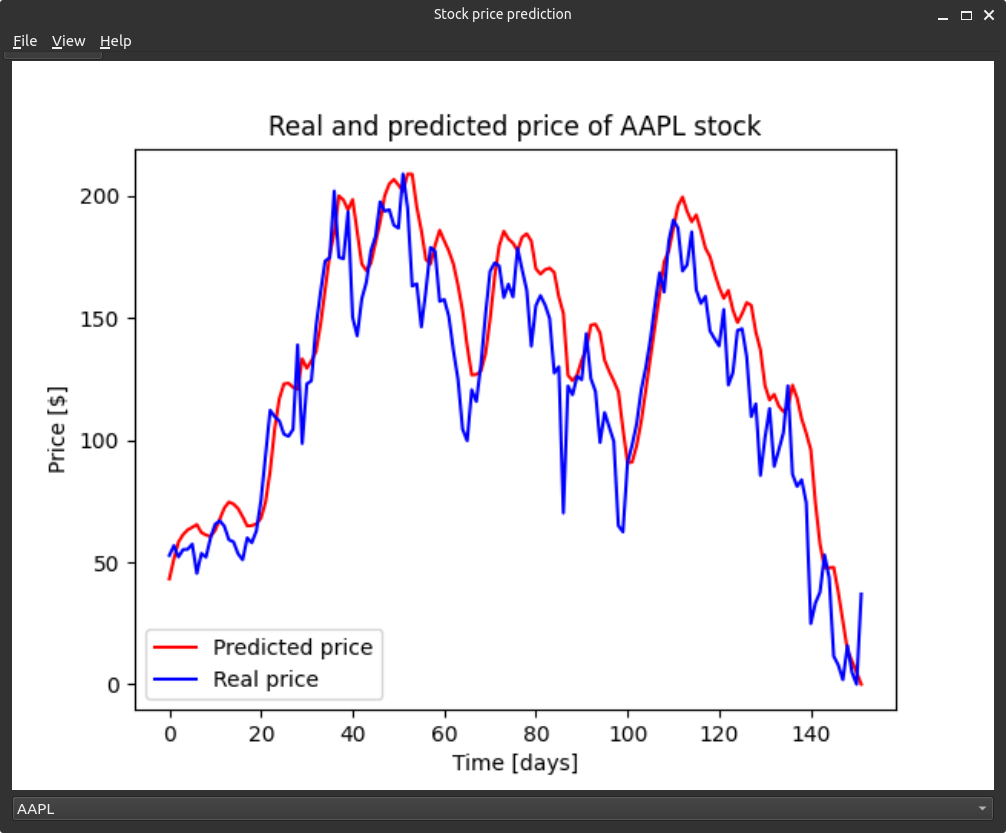
\includegraphics[width=0.5\textwidth]{./graf/MainWindow.png}
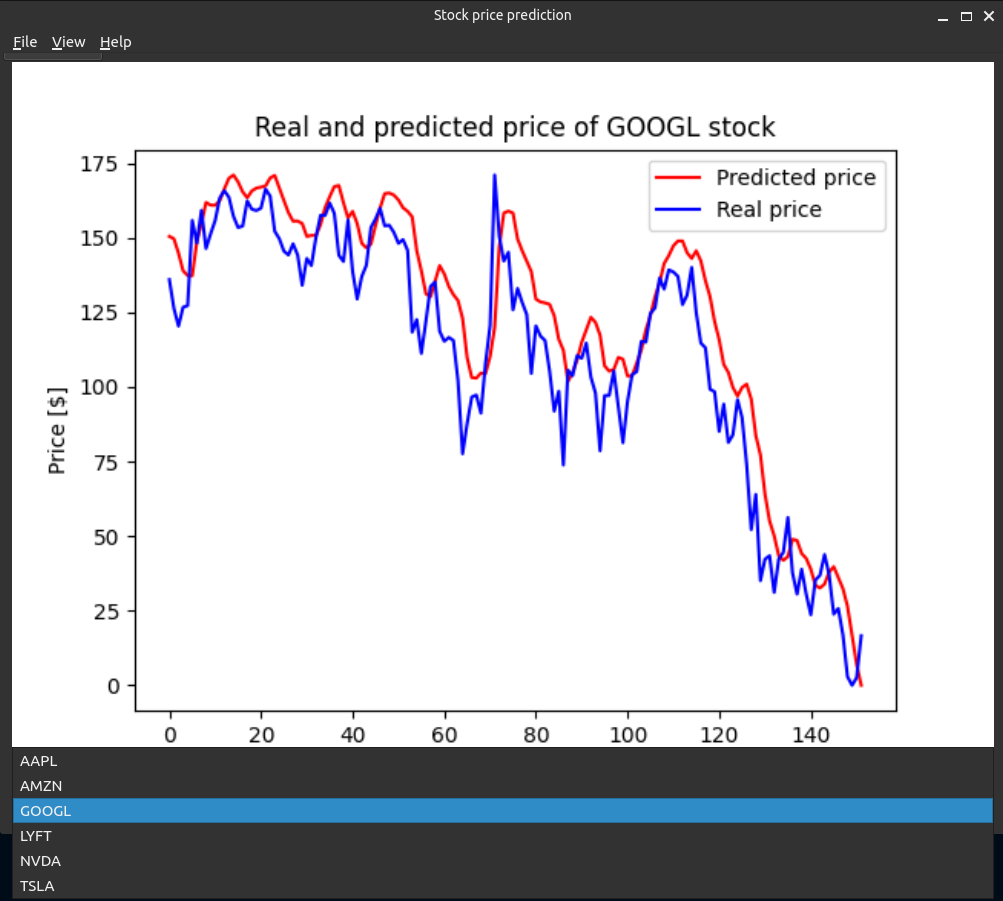
\includegraphics[width=0.5\textwidth]{./graf/MainWindow_select.png}
\caption{Main window of stock price prediction project.}
\label{fig:label}
\end{figure}

\clearpage
\begin{figure}
\centering
\begin{lstlisting}
    # Variables
    # company_name = 'AAPL' # company NASDAQ name
    price_type = 'open' # open, close, high, low, volume
    epochs = 15

    # Time interval
    startDate = '2021-06-01'
    endDate = '2022-06-01'
    interval = 'daily' # daily, weekly or monthly

    # Shape of input data
    chunkSize = 100

    # Company name dict
    company_name = ['AAPL', 'AMZN', 'GOOGL', 'LYFT', 'NVDA', 'TSLA']
\end{lstlisting}
\caption{Neural network's parameters.}
\label{fig:pseudocode:listings}
\end{figure}

%%%%%%%%%%%%%%%%%%%%%
% FIGURE FROM FILE
%
%\begin{figure}
%\centering
%
\includegraphics[width=0.5\textwidth]{./graf/politechnika_sl_logo_bw_pion_en.pdf}
%\caption{Caption of a figure is always below the figure.}
%\label{fig:label}
%\end{figure}
%Fig. \ref{fig:label} presents …
%%%%%%%%%%%%%%%%%%%%%
%
%%%%%%%%%%%%%%%%%%%%
%% SUBFIGURES
%
%\begin{figure}
%\centering
%\begin{subfigure}{0.4\textwidth}
%    
\includegraphics[width=\textwidth]{./graf/politechnika_sl_logo_bw_pion_en.pdf}
%    \caption{Upper left figure.}
%    \label{fig:upper-left}
%\end{subfigure}
%\hfill
%\begin{subfigure}{0.4\textwidth}
%    
\includegraphics[width=\textwidth]{./graf/politechnika_sl_logo_bw_pion_en.pdf}
%    \caption{Upper right figure.}
%    \label{fig:upper-right}
%\end{subfigure}
%
%\begin{subfigure}{0.4\textwidth}
%    
\includegraphics[width=\textwidth]{./graf/politechnika_sl_logo_bw_pion_en.pdf}
%    \caption{Lower left figure.}
%    \label{fig:lower-left}
%\end{subfigure}
%\hfill
%\begin{subfigure}{0.4\textwidth}
%    
\includegraphics[width=\textwidth]{./graf/politechnika_sl_logo_bw_pion_en.pdf}
%    \caption{Lower right figure.}
%    \label{fig:lower-right}
%\end{subfigure}
%        
%\caption{Common caption for all subfigures.}
%\label{fig:subfigures}
%\end{figure}
%Fig. \ref{fig:subfigures} presents very important information, eg. Fig. \ref{fig:upper-right} is an upper right subfigure.
%%%%%%%%%%%%%%%%%%%%%
 

% TODO
\chapter{Internal specification}

\begin{itemize}
\item concept of the system
\item system architecture
\item description of data structures (and data bases)
\item components, modules, libraries, resume of important classes (if used)
\item resume of important algorithms (if used)
\item details of implementation of selected parts
\item applied design patterns
\item UML diagrams
\end{itemize}



% % % % % % % % % % % % % % % % % % % % % % % % % % % % % % % % % % % 
% To use the minted packages uncomment the package import in        %
% file config/settings.tex :  \usepackage{minted}                   %
% and compile with the shell escape                                 %
% pdflatex -shell-escape main                                       %
% % % % % % % % % % % % % % % % % % % % % % % % % % % % % % % % % % % 


Use special environments for inline code, eg  \lstinline|int a;| (package \texttt{listings})% or  \mintinline{C++}|int a;| (package \texttt{minted})
. Longer parts of code put in the figure environment, eg. code in Fig. \ref{fig:pseudocode:listings}% and Fig. \ref{fig:pseudocode:minted}
. Very long listings–move to an appendix.


\clearpage
\begin{figure}
\centering
\begin{lstlisting}
class test : public basic
{
    public:
      test (int a);
      friend std::ostream operator<<(std::ostream & s, 
                                     const test & t);
    protected:
      int _a;  
      
};
\end{lstlisting}
\caption{Pseudocode in \texttt{listings}.}
\label{fig:pseudocode:listings}
\end{figure}

%\begin{figure}
%\centering
%\begin{minted}[linenos,frame=lines]{c++}
%class test : public basic
%{
%    public:
%      test (int a);
%      friend std::ostream operator<<(std::ostream & s, 
%                                     const test & t);
%    protected:
%      int _a;  
%      
%};
%\end{minted}
%\caption{Pseudocode in \texttt{minted}.}
%\label{fig:pseudocode:minted}
%\end{figure}


 

% TODO
\chapter{Verification and validation}
\begin{itemize}
\item testing paradigm (eg V model)
\item test cases, testing scope (full / partial)
\item detected and fixed bugs
\item results of experiments (optional)
\end{itemize}

In order to test the best possible configuration options for the model, many different configurations have been tested.
\par
\bigskip
Model1 - chunkSize: 20, time interval: 1 year, epochs: 5, trained on AAPL\par
Model2 - chunkSize: 20, time interval: 1 year, epochs: 10, trained on AAPL\par
Model3 - chunkSize: 20, time interval: 1 year, epochs: 15, trained on AAPL\par
\par
\bigskip
Model4 - chunkSize: 50, time interval: 1 year, epochs: 5, trained on AAPL\par
Model5 - chunkSize: 50, time interval: 1 year, epochs: 10, trained on AAPL\par
Model6 - chunkSize: 50, time interval: 1 year, epochs: 15, trained on AAPL\par
\par
\bigskip
Model7 - chunkSize: 100, time interval: 1 year, epochs: 5, trained on AAPL\par
Model8 - chunkSize: 100, time interval: 1 year, epochs: 10, trained on AAPL\par
Model9 - chunkSize: 100, time interval: 1 year, epochs: 15, trained on AAPL\par
\par
\bigskip

\section{Different models}

In order to verify that the system works correctly, the tests were performed on different inputs and parameters to obtain the most accurate results. The opening prices of shares of the largest companies on the United States stock market were used as input data. Various time periods were tested to carry out the verification reliably. The created solution predicted stock prices only for the nearest period of time, and then the obtained results were compared with actual historical data. In order to clearly illustrate the results, everything is presented on graphs.

In this section, the general work of the presented neural network has been tested. Only one day in the future has been predicted here in order to visualize whether the output data looks real and probable. On the graph, many intervals predicting a single day in the future are presented and accumulated on a single graph.

Firstly, the biggest tech companies were chosen as the first tested model and were trained on tech companies.

Analyzing the presented graphs, a few conclusions could be drawn.


\subsection{Model 1}

Model1 - chunkSize: 20, time interval: 1 year, epochs: 5, trained on AAPL\par\bigskip
After a quick look at the charts,  one can notice that the predicted prices are pretty close to the real prices. From this, it can be concluded that the price prediction model on the US stock market works. Further investigation may reveal which parameters work best.
In the first model, one can see that the red line is placed quite prominently above the blue line. Moreover, some anomalies (for example, sudden sharp drops or price increases) are slightly delayed in the red line relative to the blue line. We may also notice that very rapid changes (for example, large one-day price swings) noticeable in the blue line are not visible in the red line.
\clearpage
\begin{figure}
% \centering
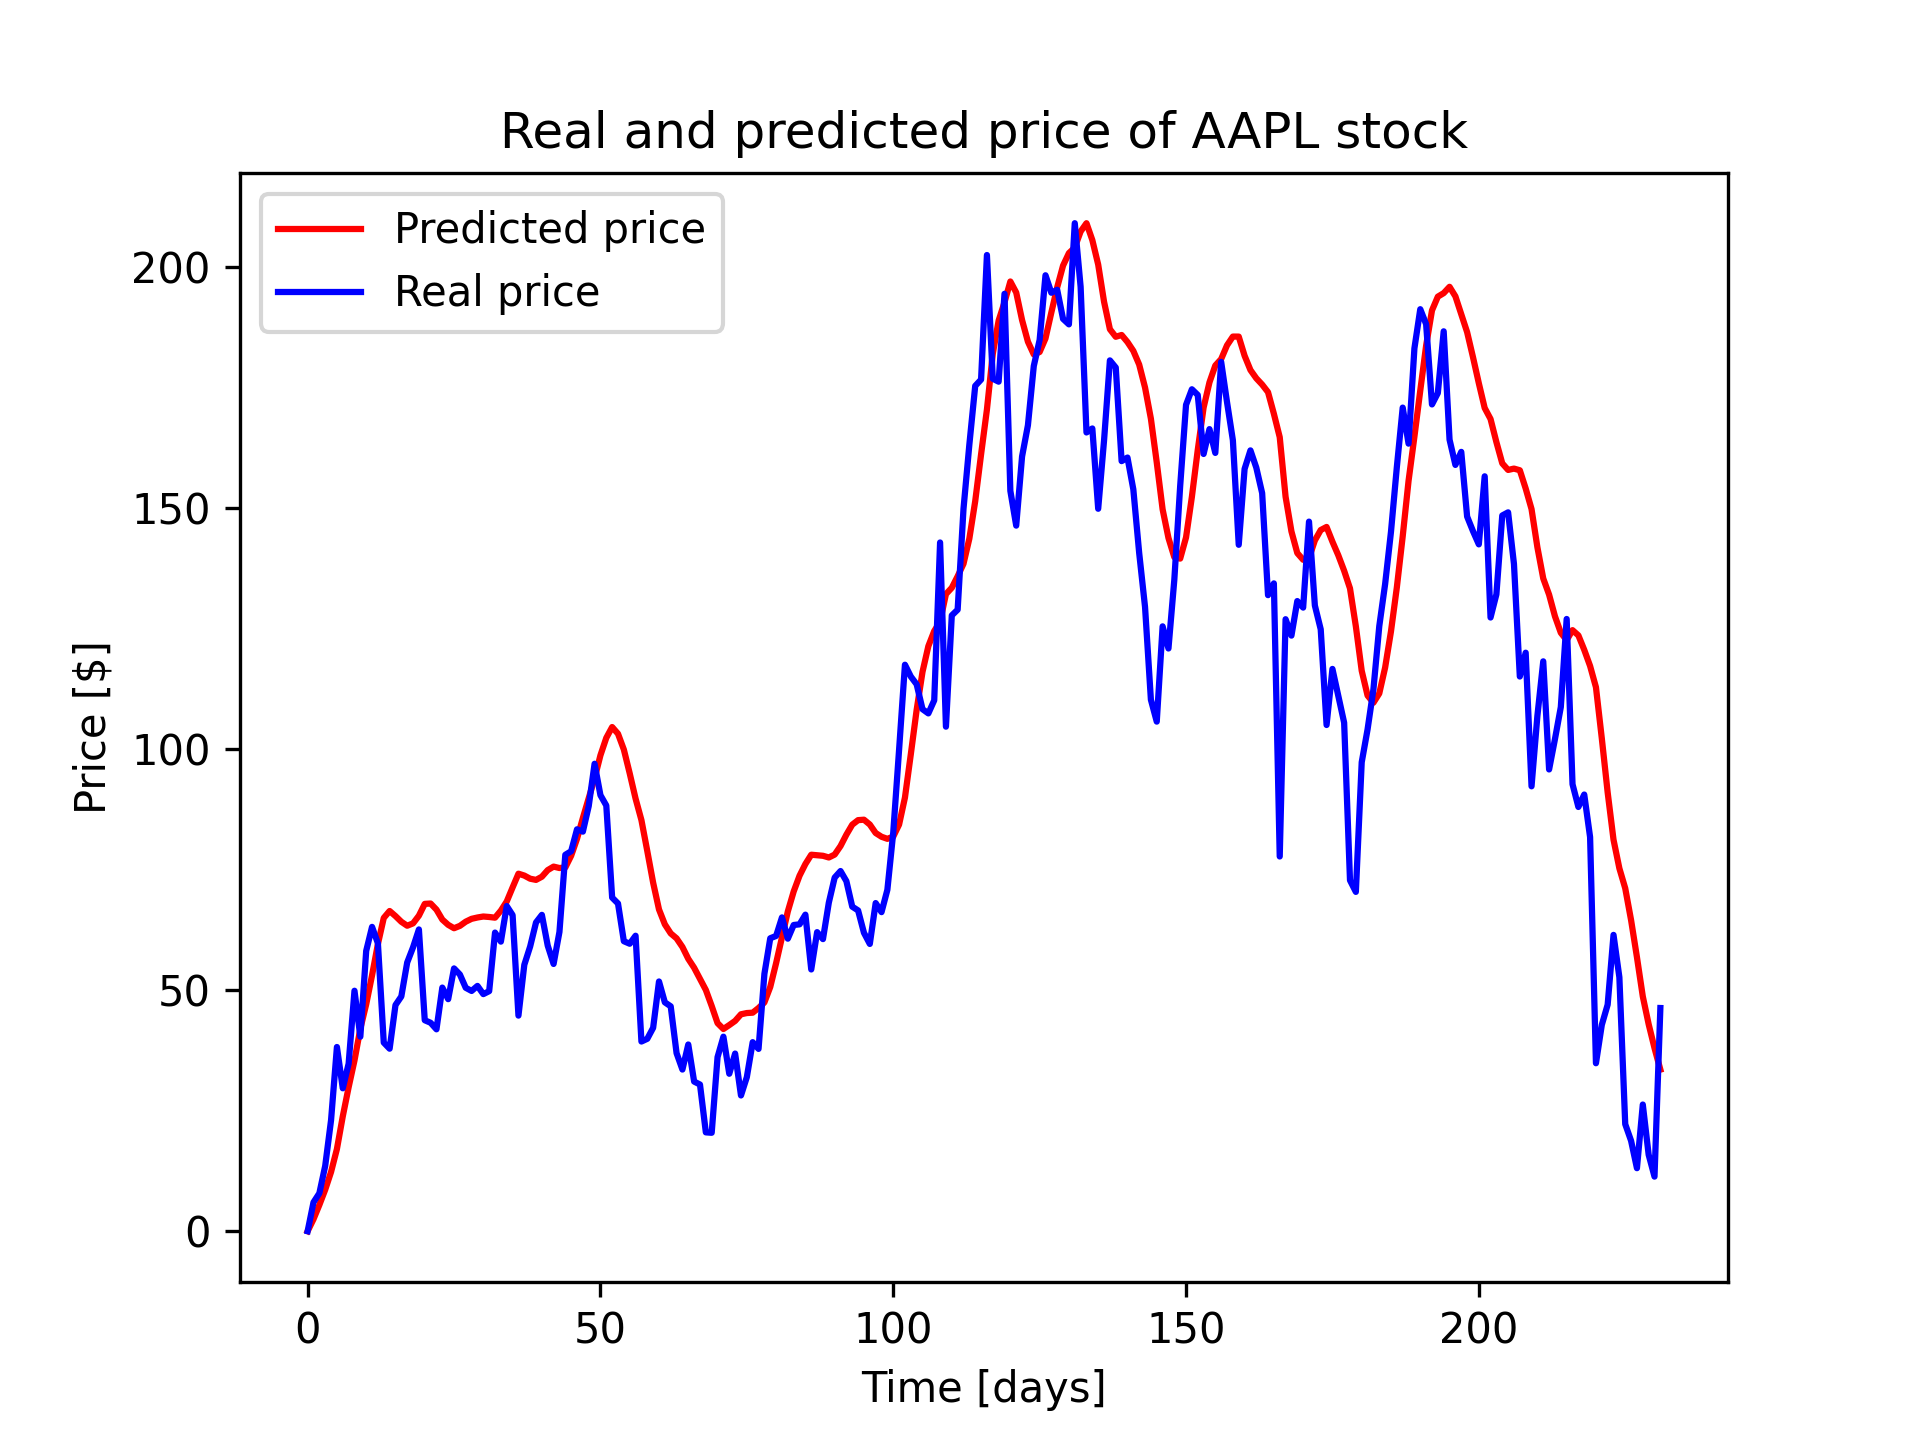
\includegraphics[width=0.5\textwidth]{./graf/model1/AAPL.png}
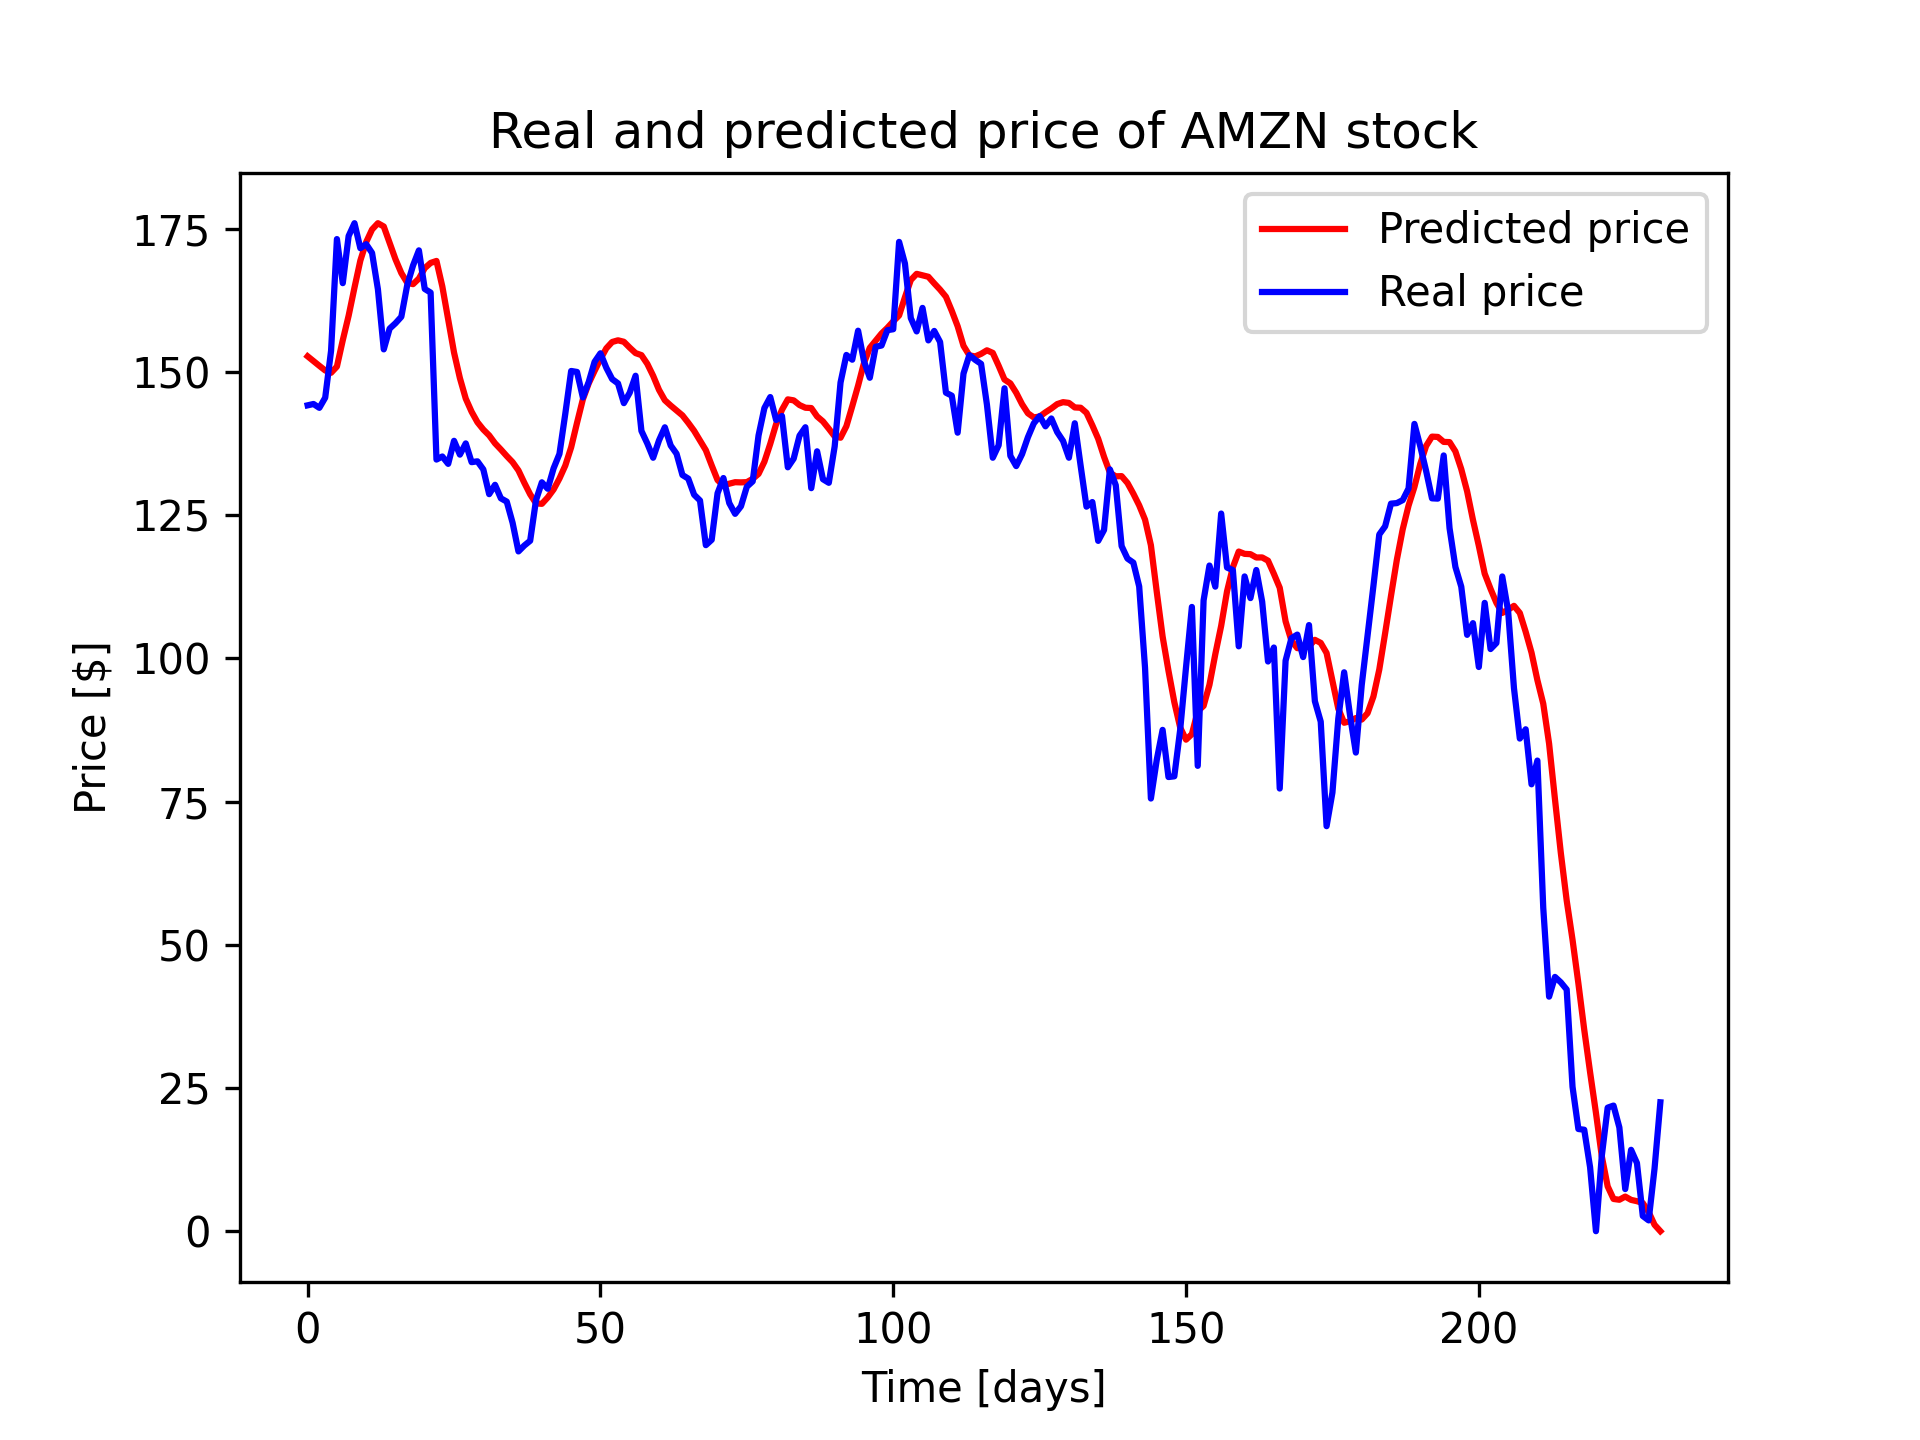
\includegraphics[width=0.5\textwidth]{./graf/model1/AMZN.png}
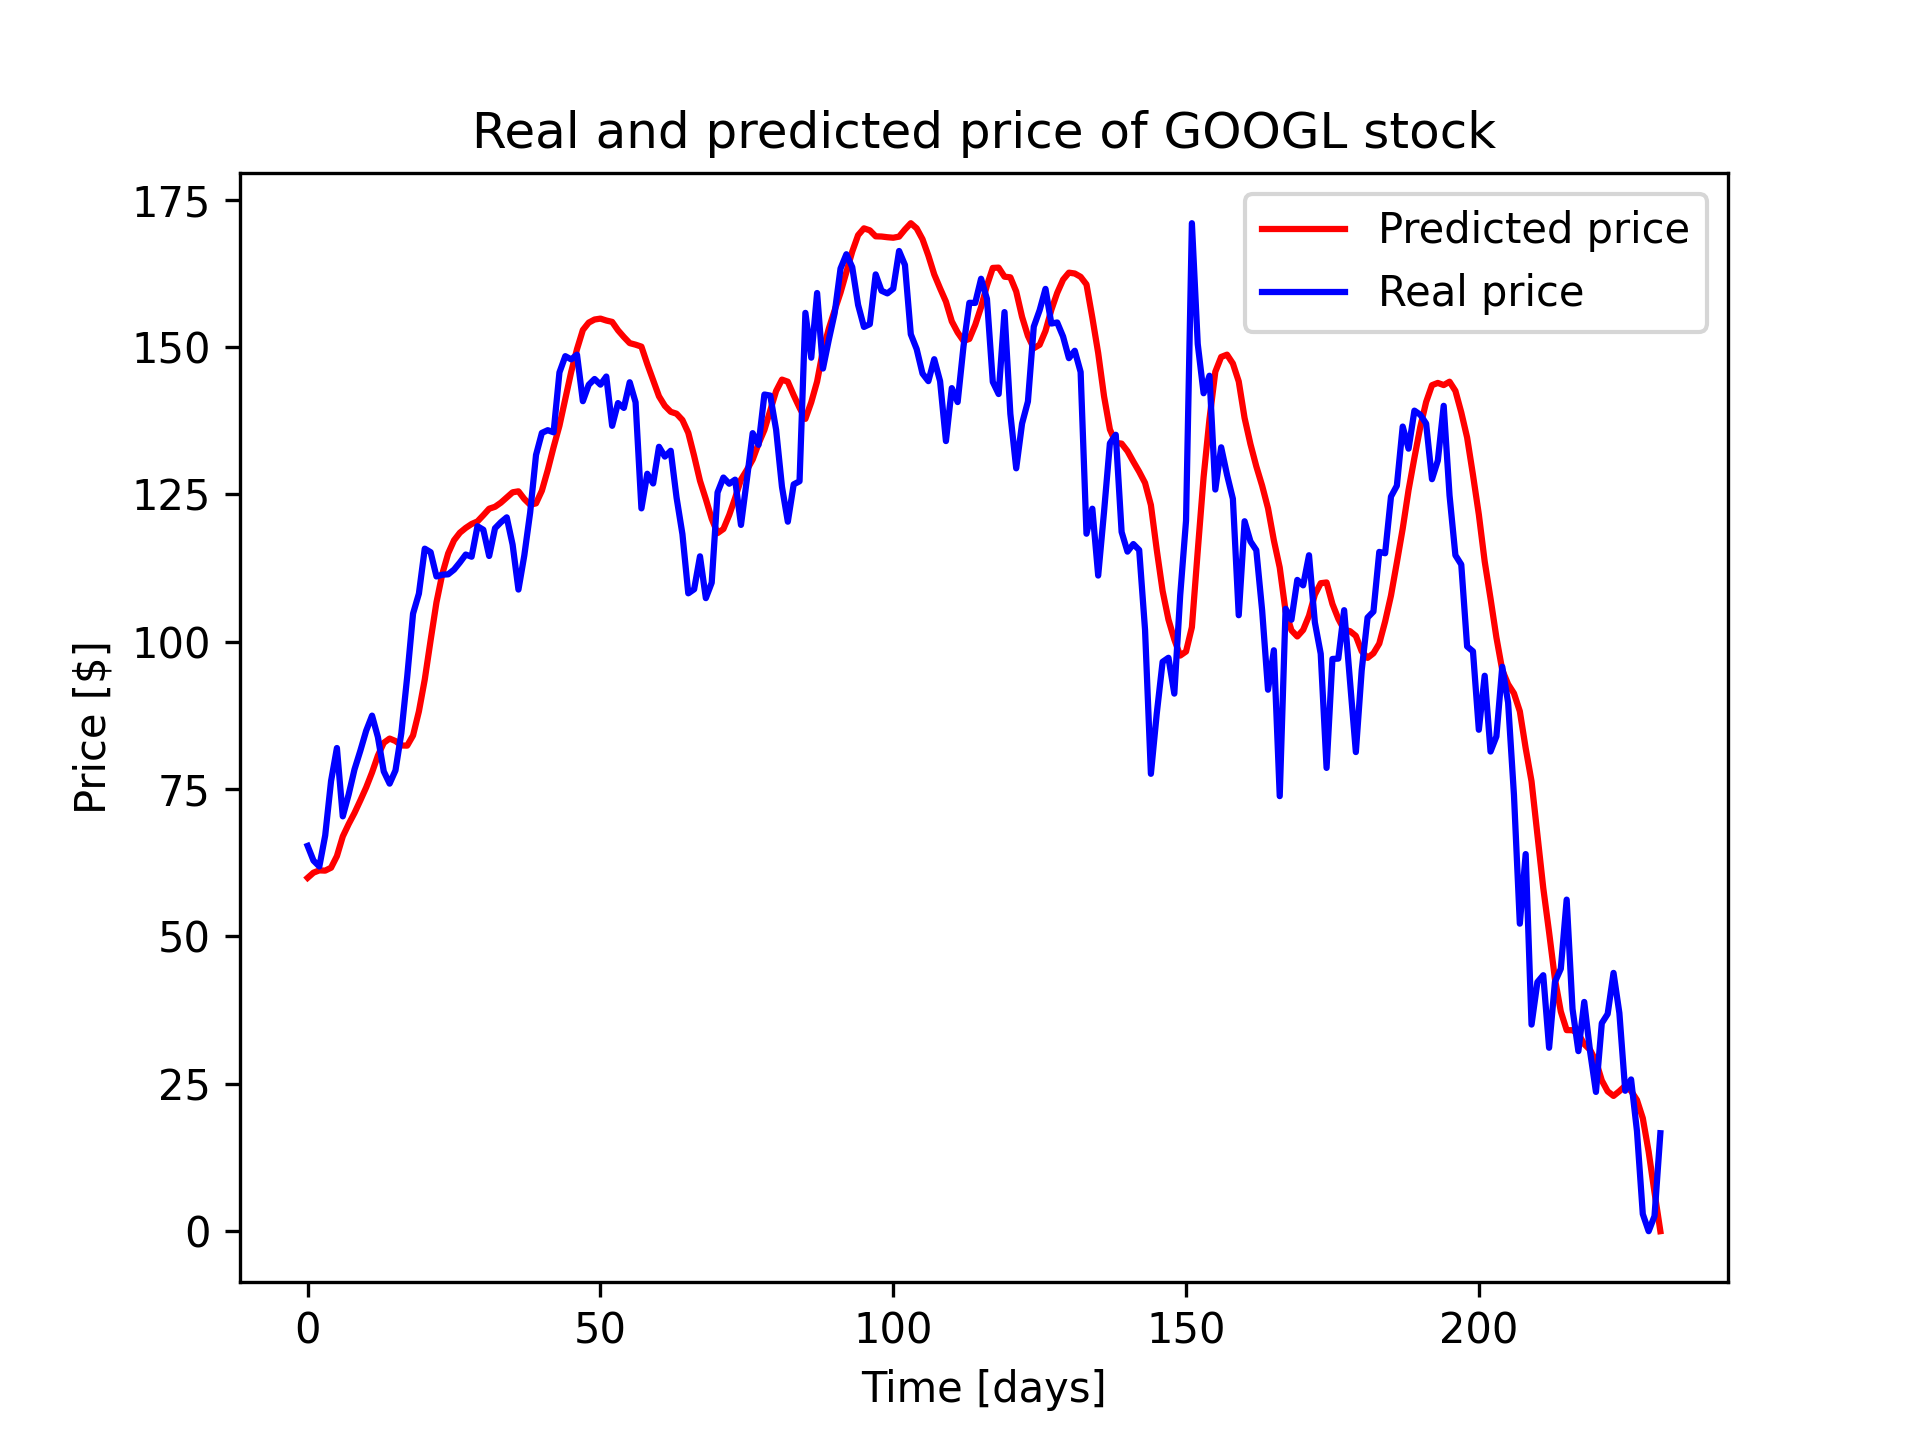
\includegraphics[width=0.5\textwidth]{./graf/model1/GOOGL.png}
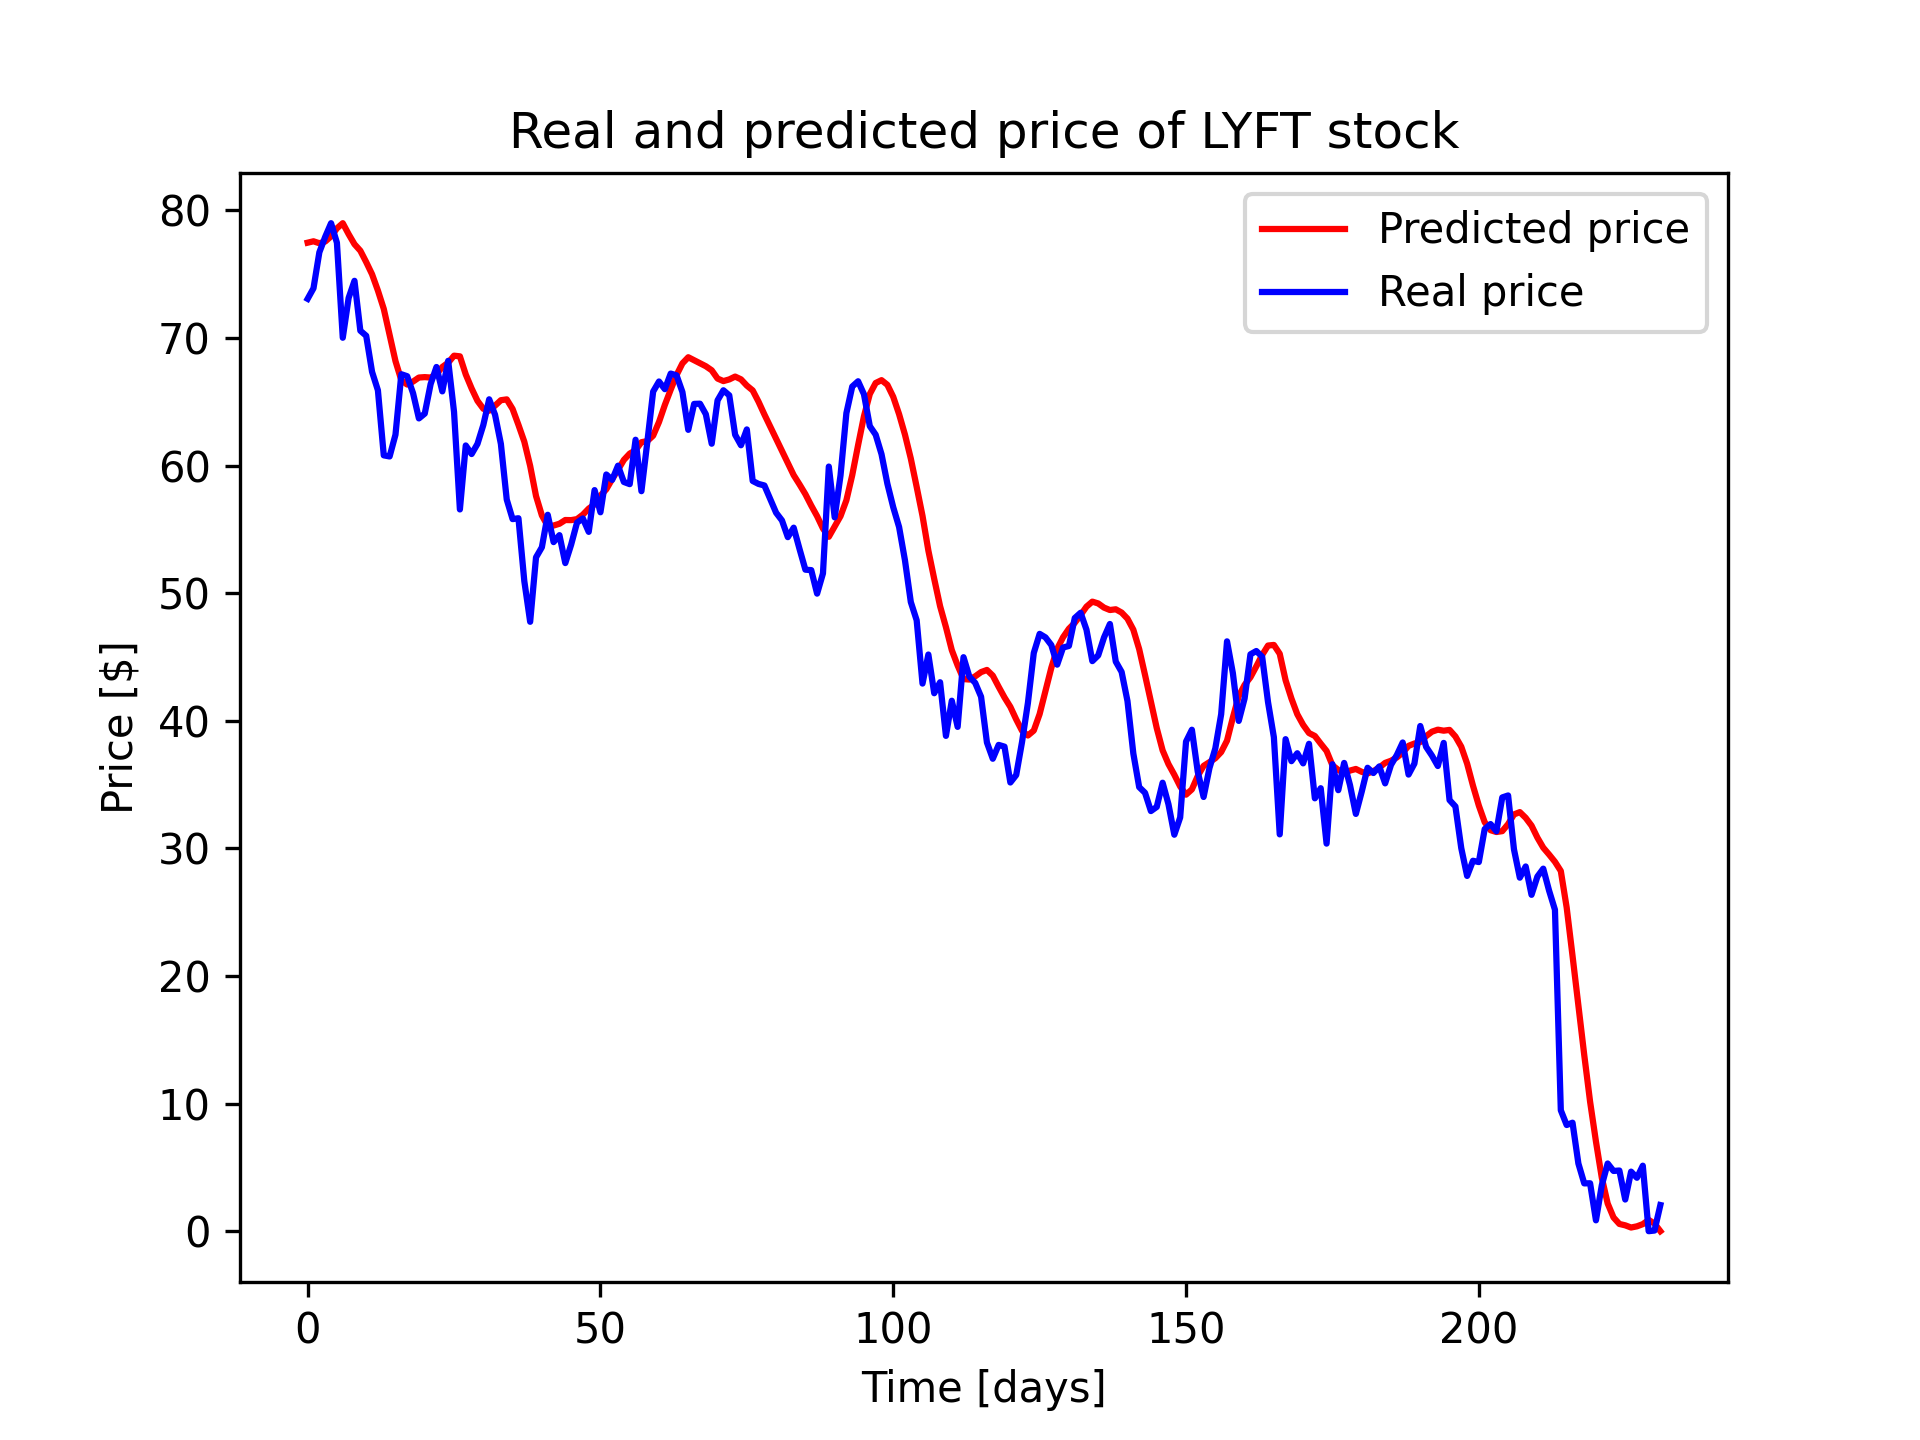
\includegraphics[width=0.5\textwidth]{./graf/model1/LYFT.png}
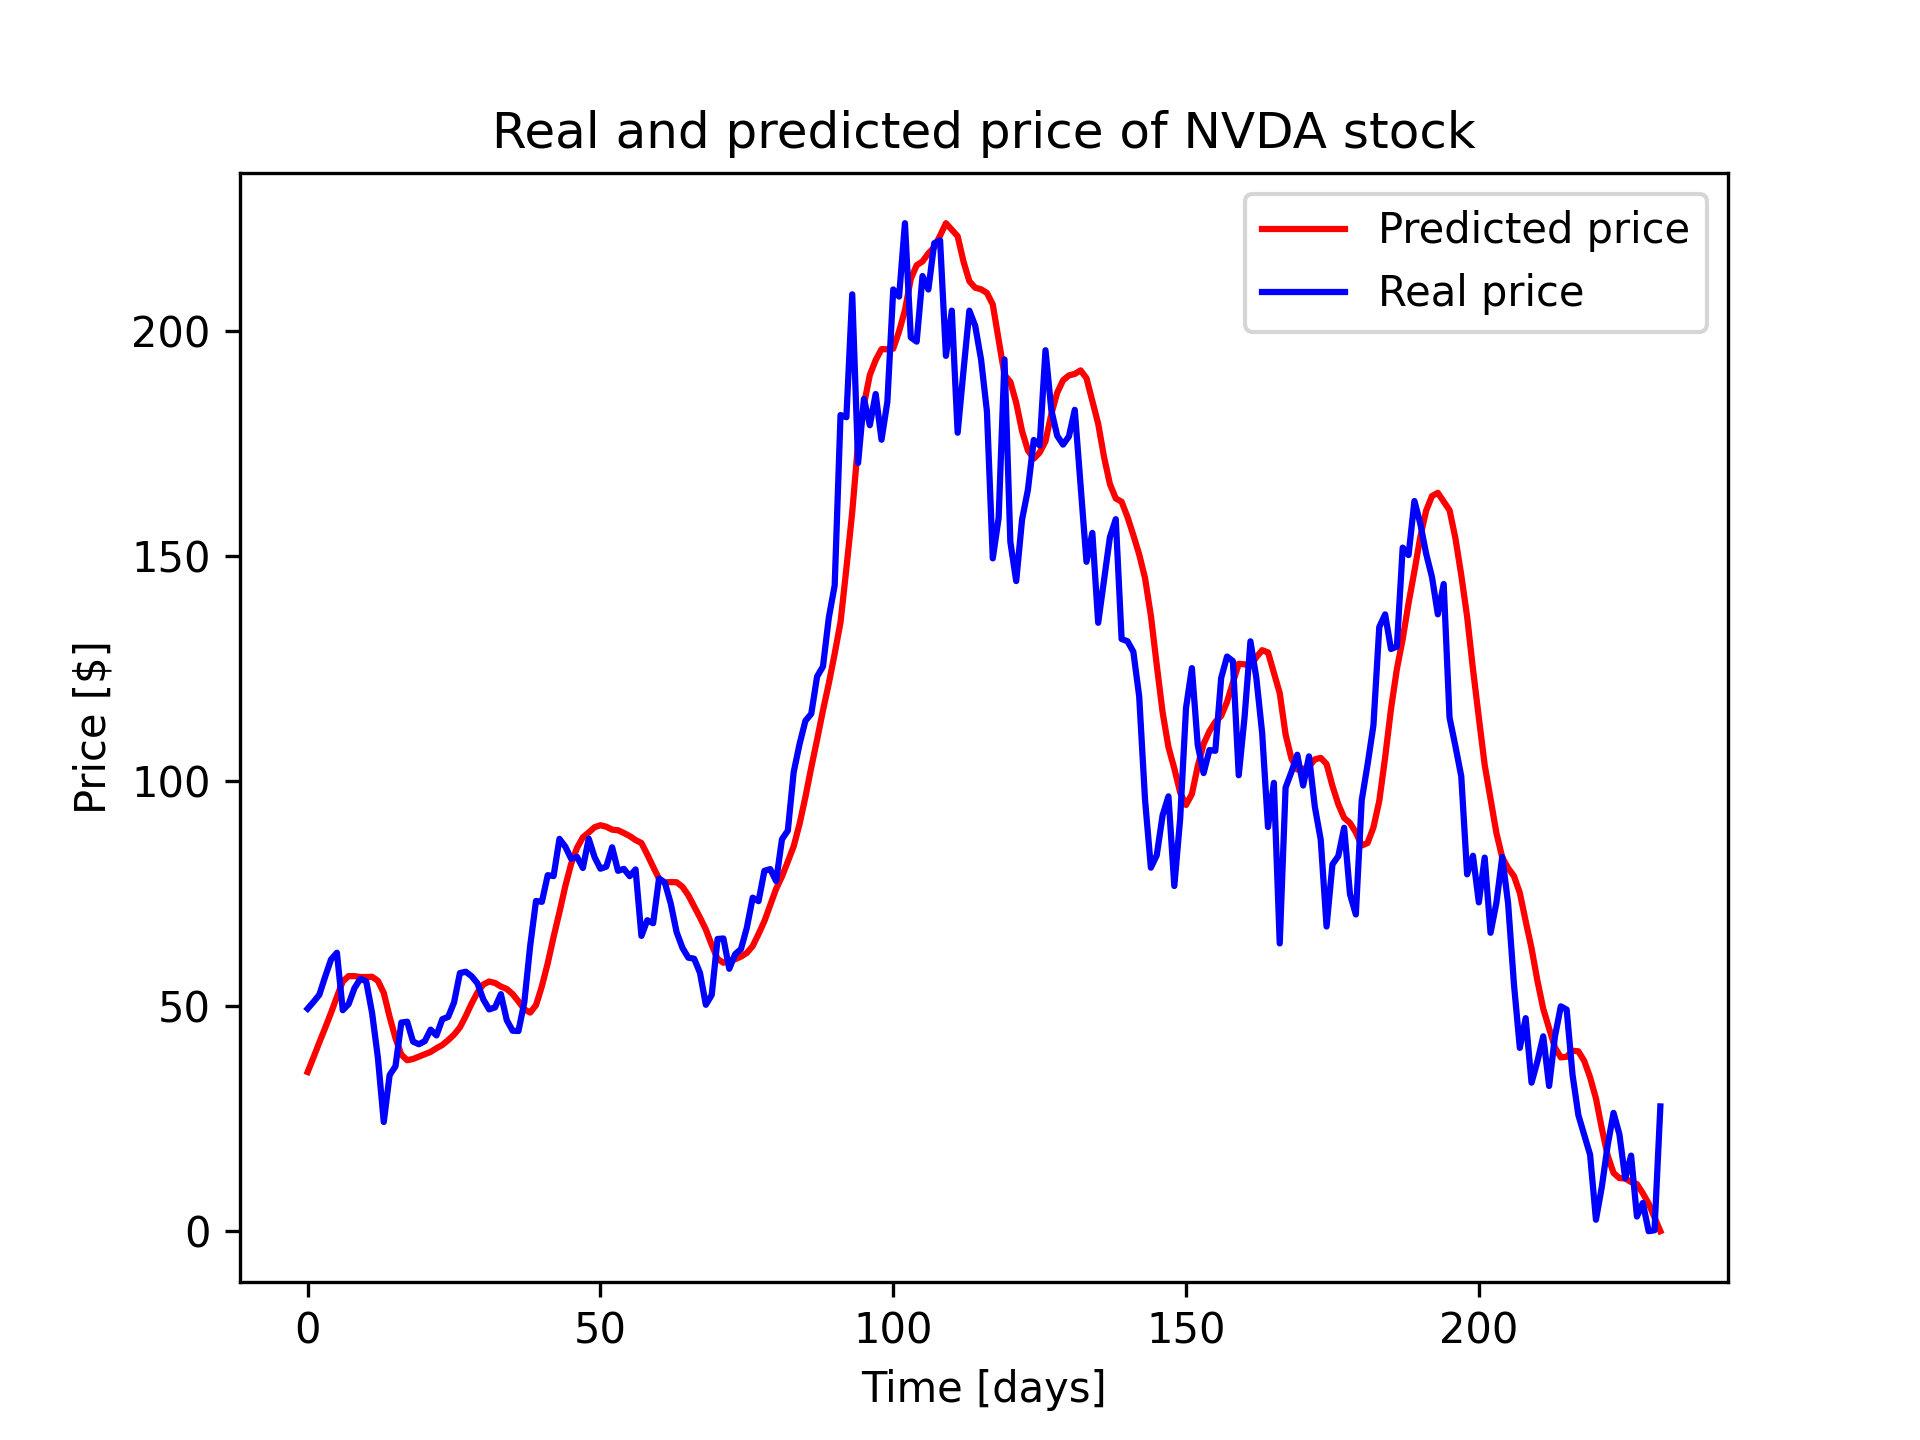
\includegraphics[width=0.5\textwidth]{./graf/model1/NVDA.png}
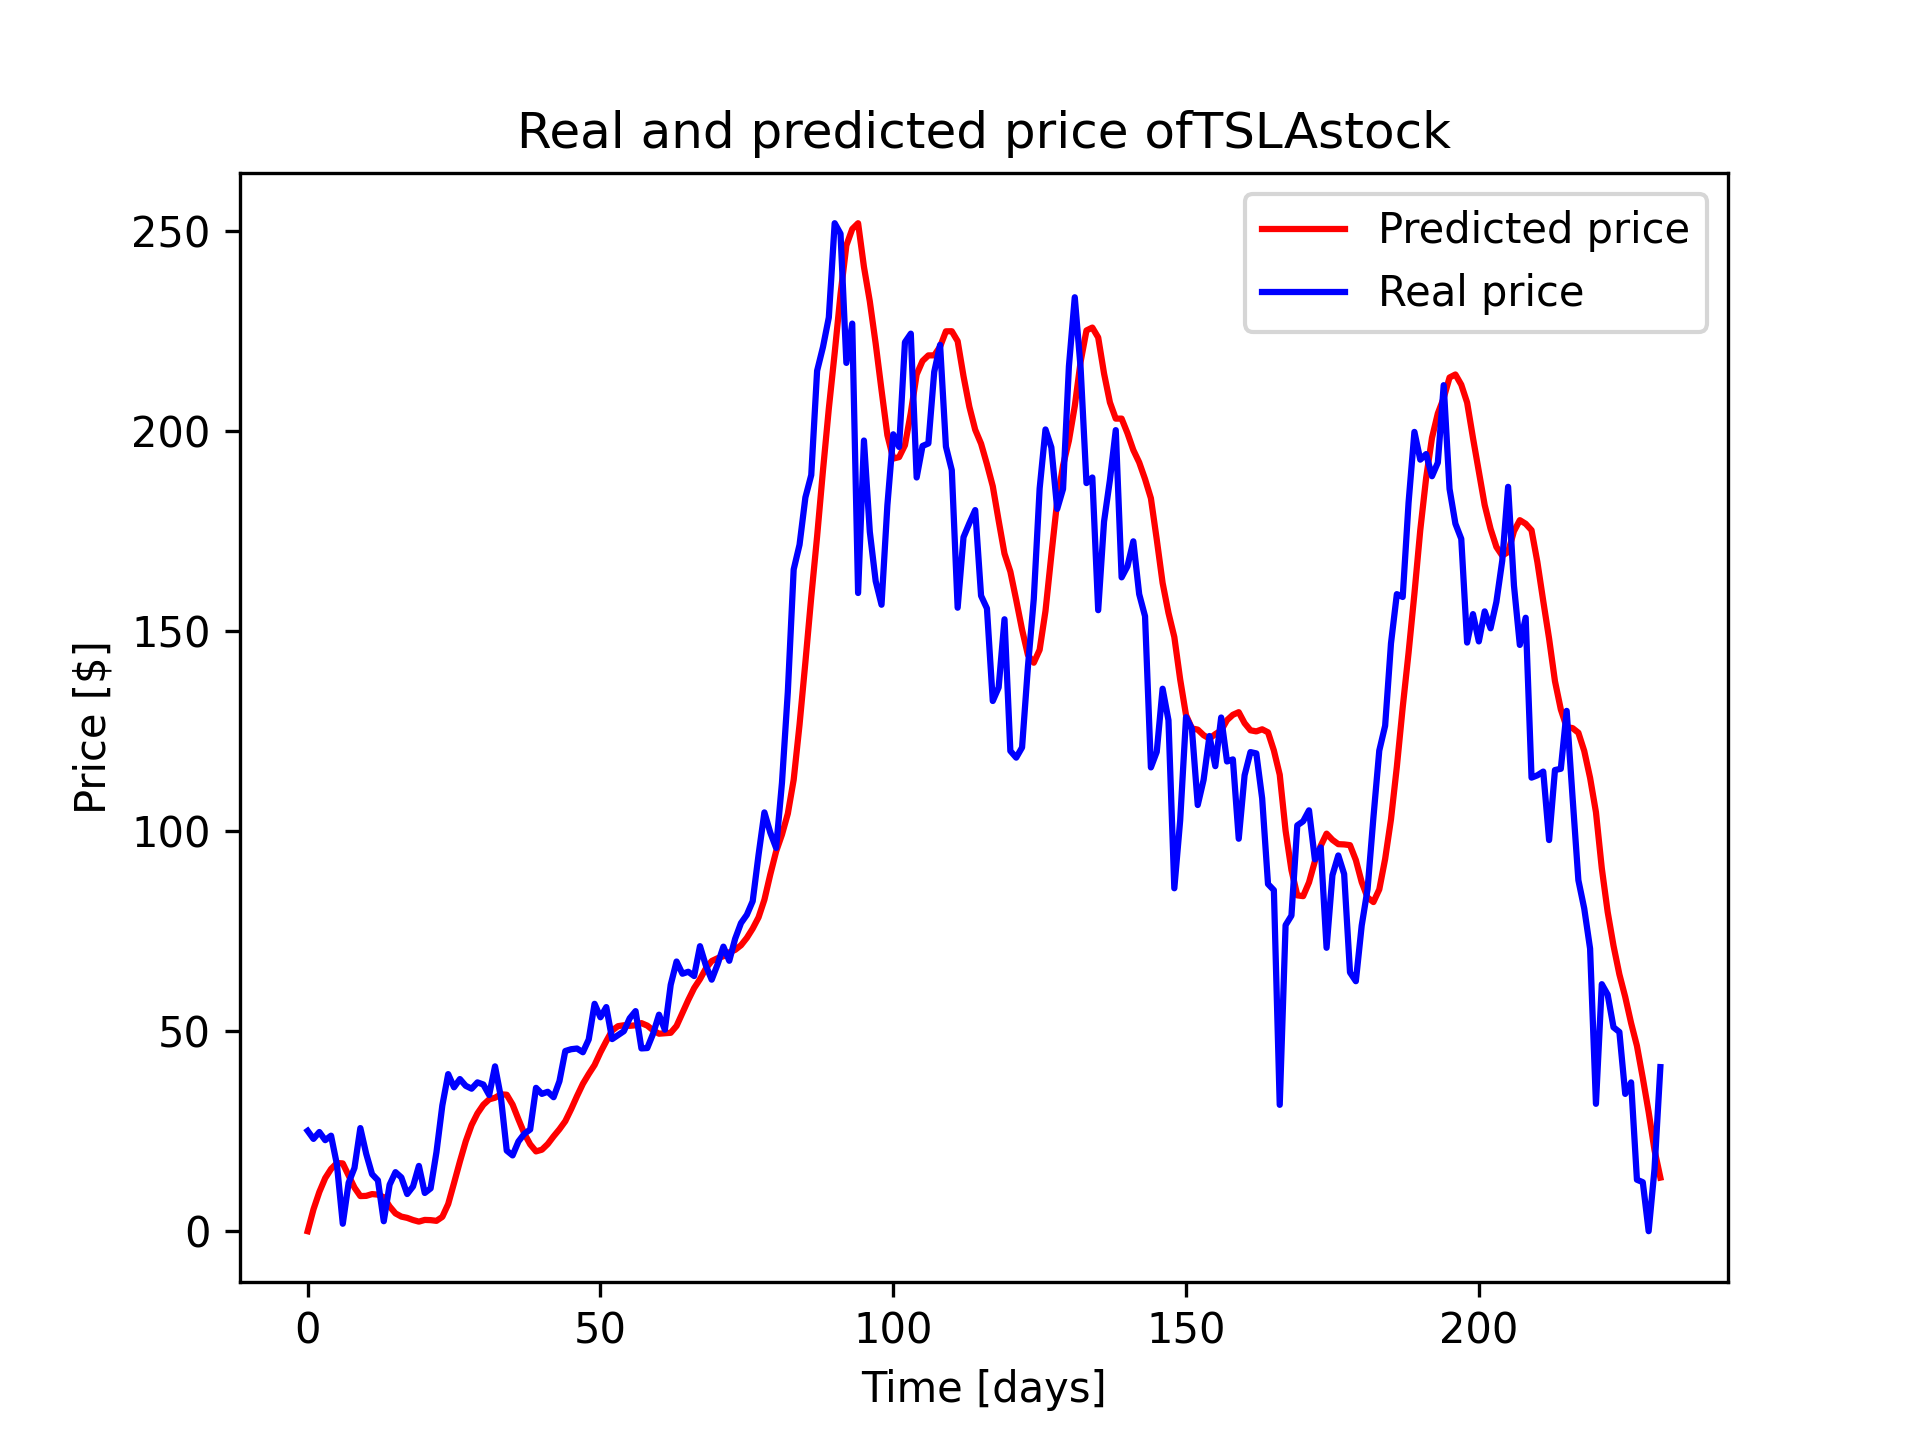
\includegraphics[width=0.5\textwidth]{./graf/model1/TSLA.png}
\caption{Real and predicted prices of the first model.}
\label{fig:label}
\end{figure} 

\clearpage
\subsection{Model 2}

Model2 - chunkSize: 20, time interval: 1 year, epochs: 10, trained on AAPL\par\bigskip
In model no. 2, it can be seen that the red line corresponding to the predicted price is slightly above
the blue line corresponding to the real price. It is worth noting that the peaks regarding the sudden
increase in the value of shares in both variants coincide. Sudden day-to-day swings are not included
in the red line, whether going up or down in the stock's value.
\par
Some anomalies, for example, sudden price spikes, are slightly delayed in the red line relative to the blue line.
Also, swift changes, for example, one-day large price fluctuations noticeable in the blue line, are invisible
in the red line.

\begin{figure}
% \centering
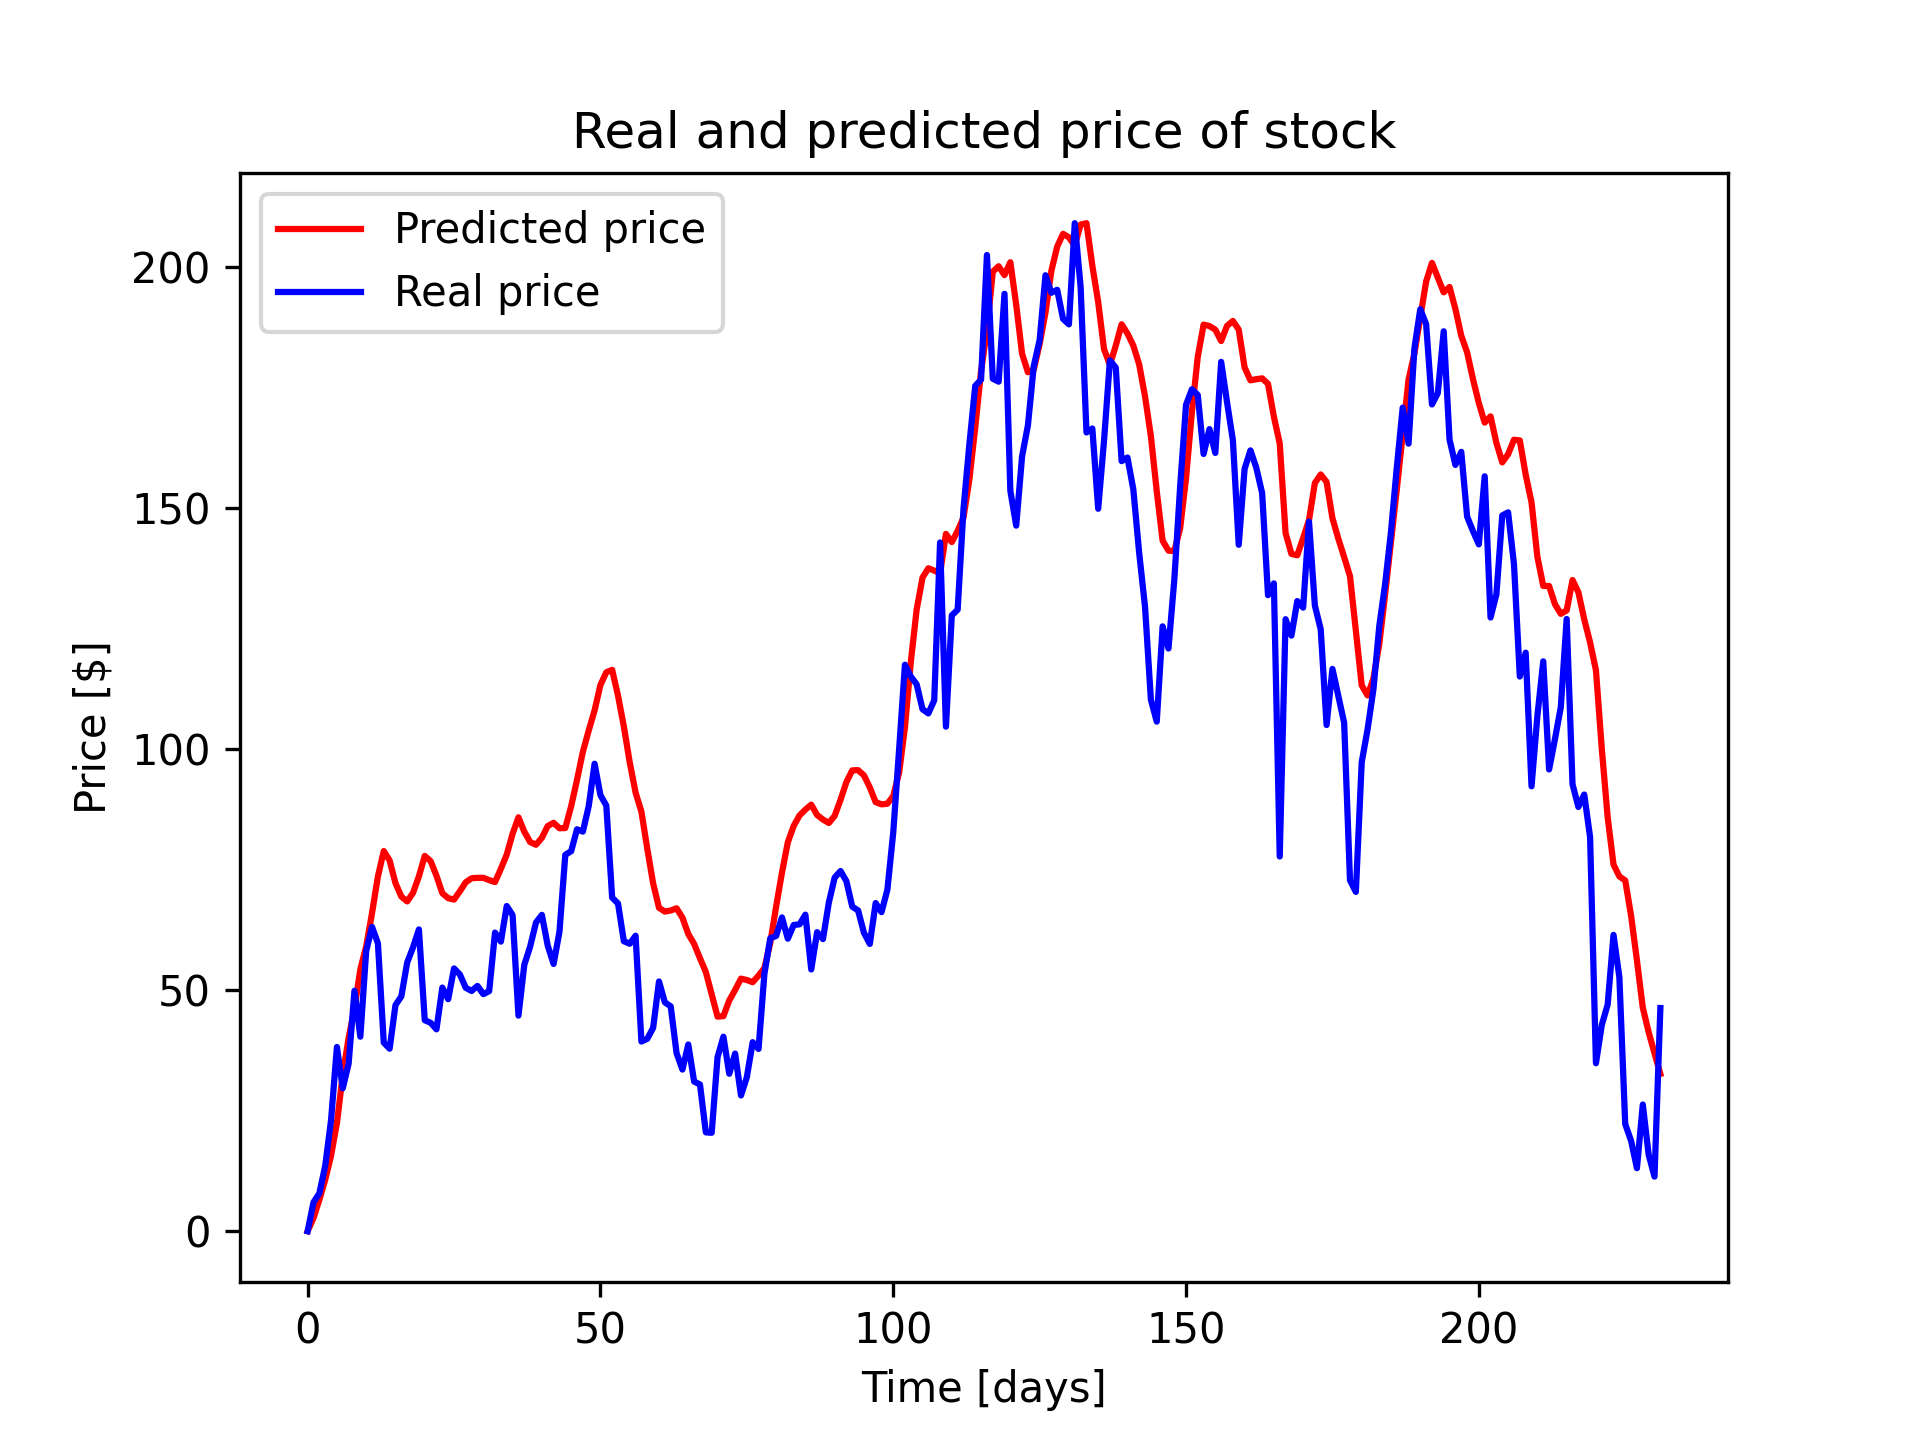
\includegraphics[width=0.5\textwidth]{./graf/model2/AAPL.png}
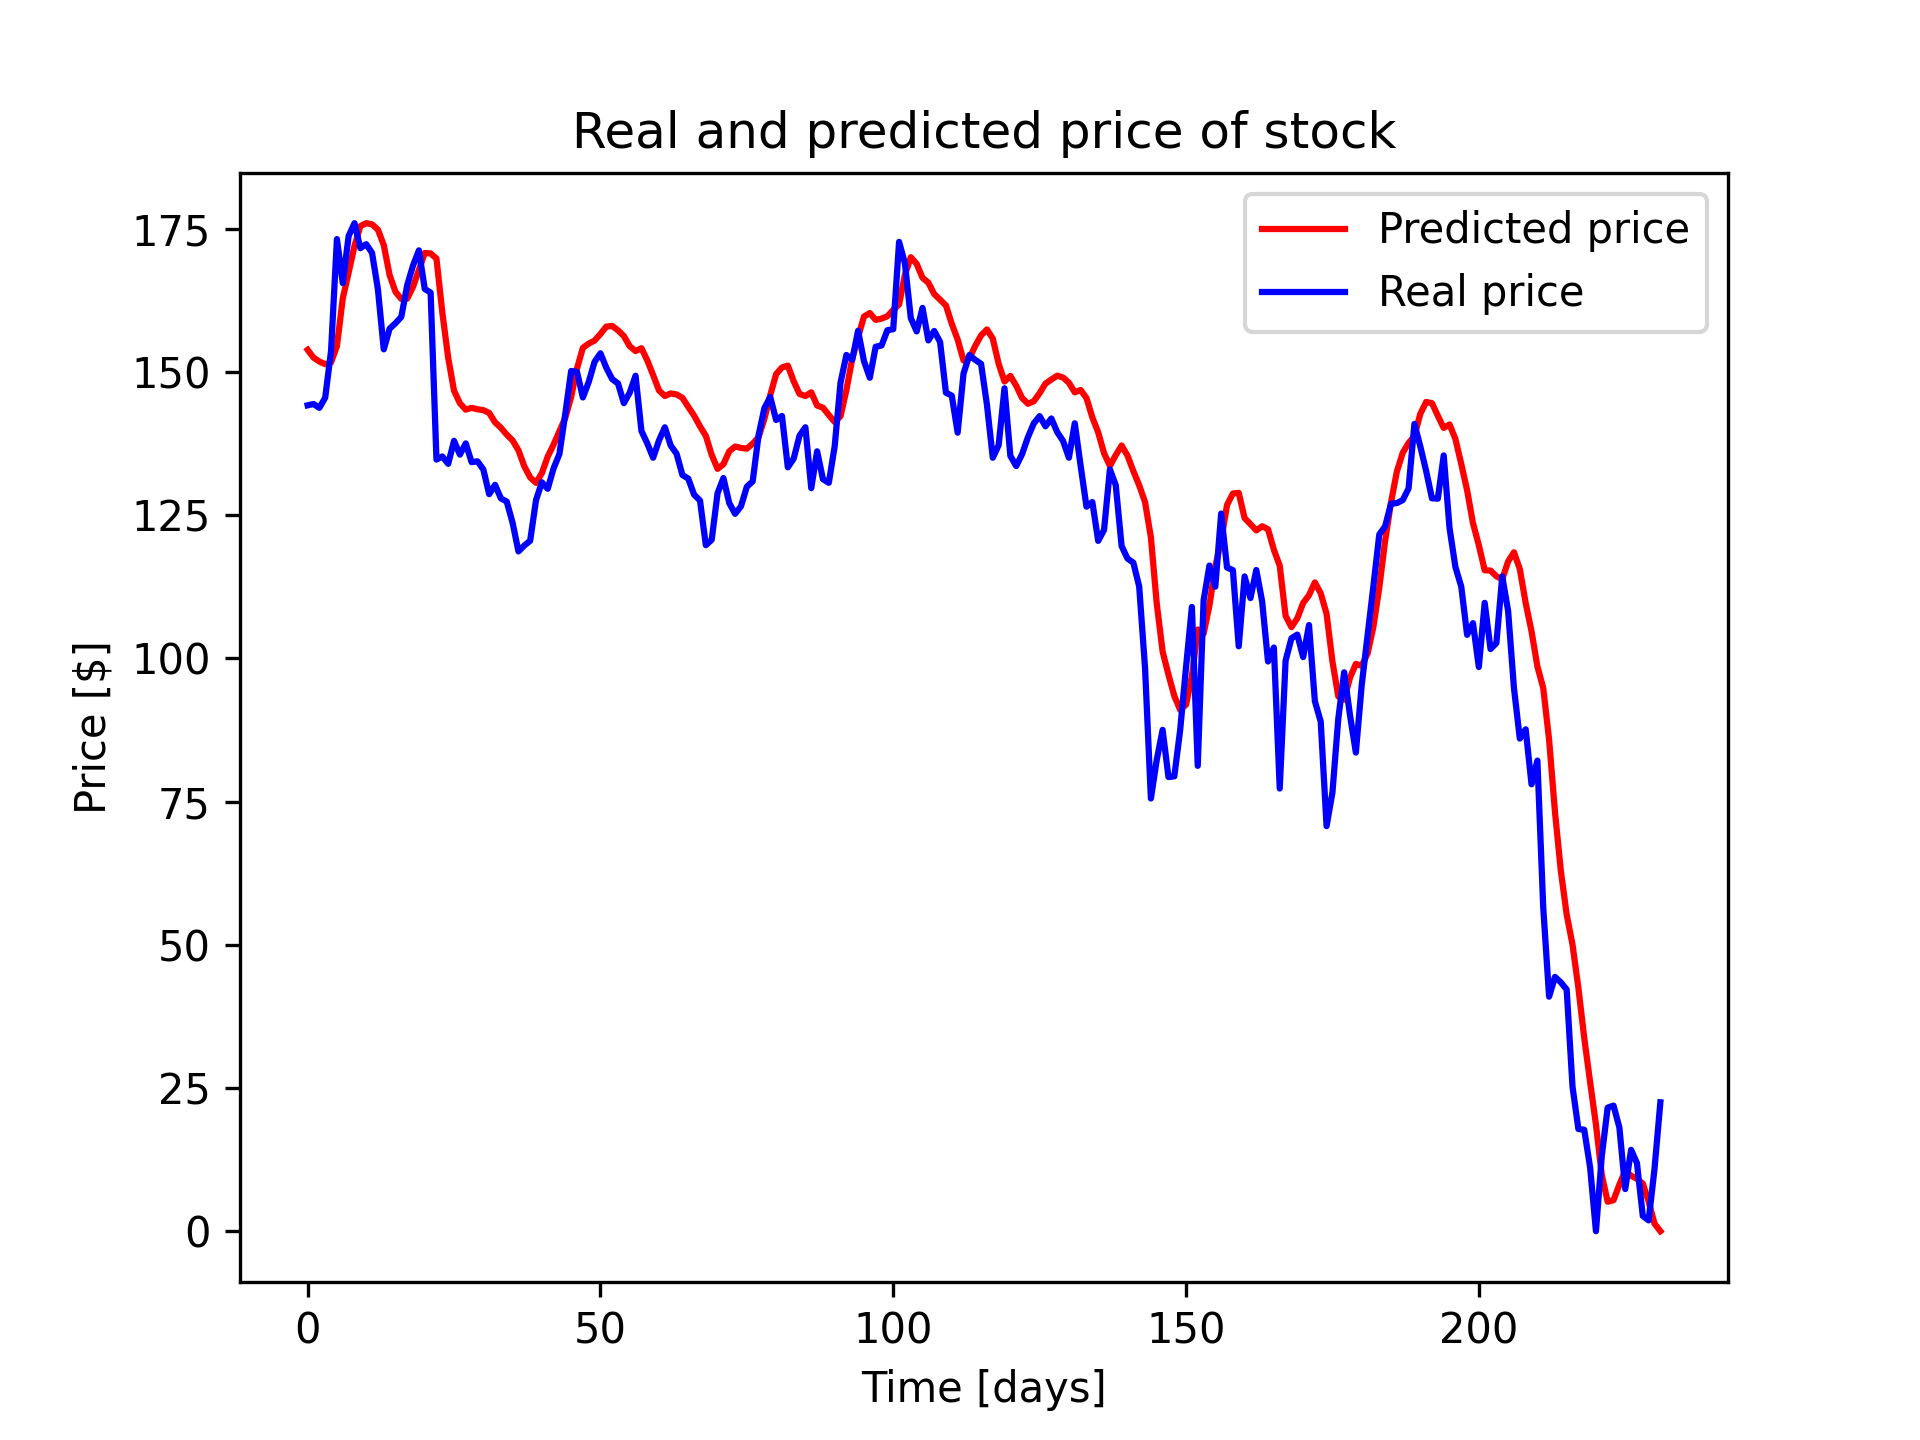
\includegraphics[width=0.5\textwidth]{./graf/model2/AMZN.png}
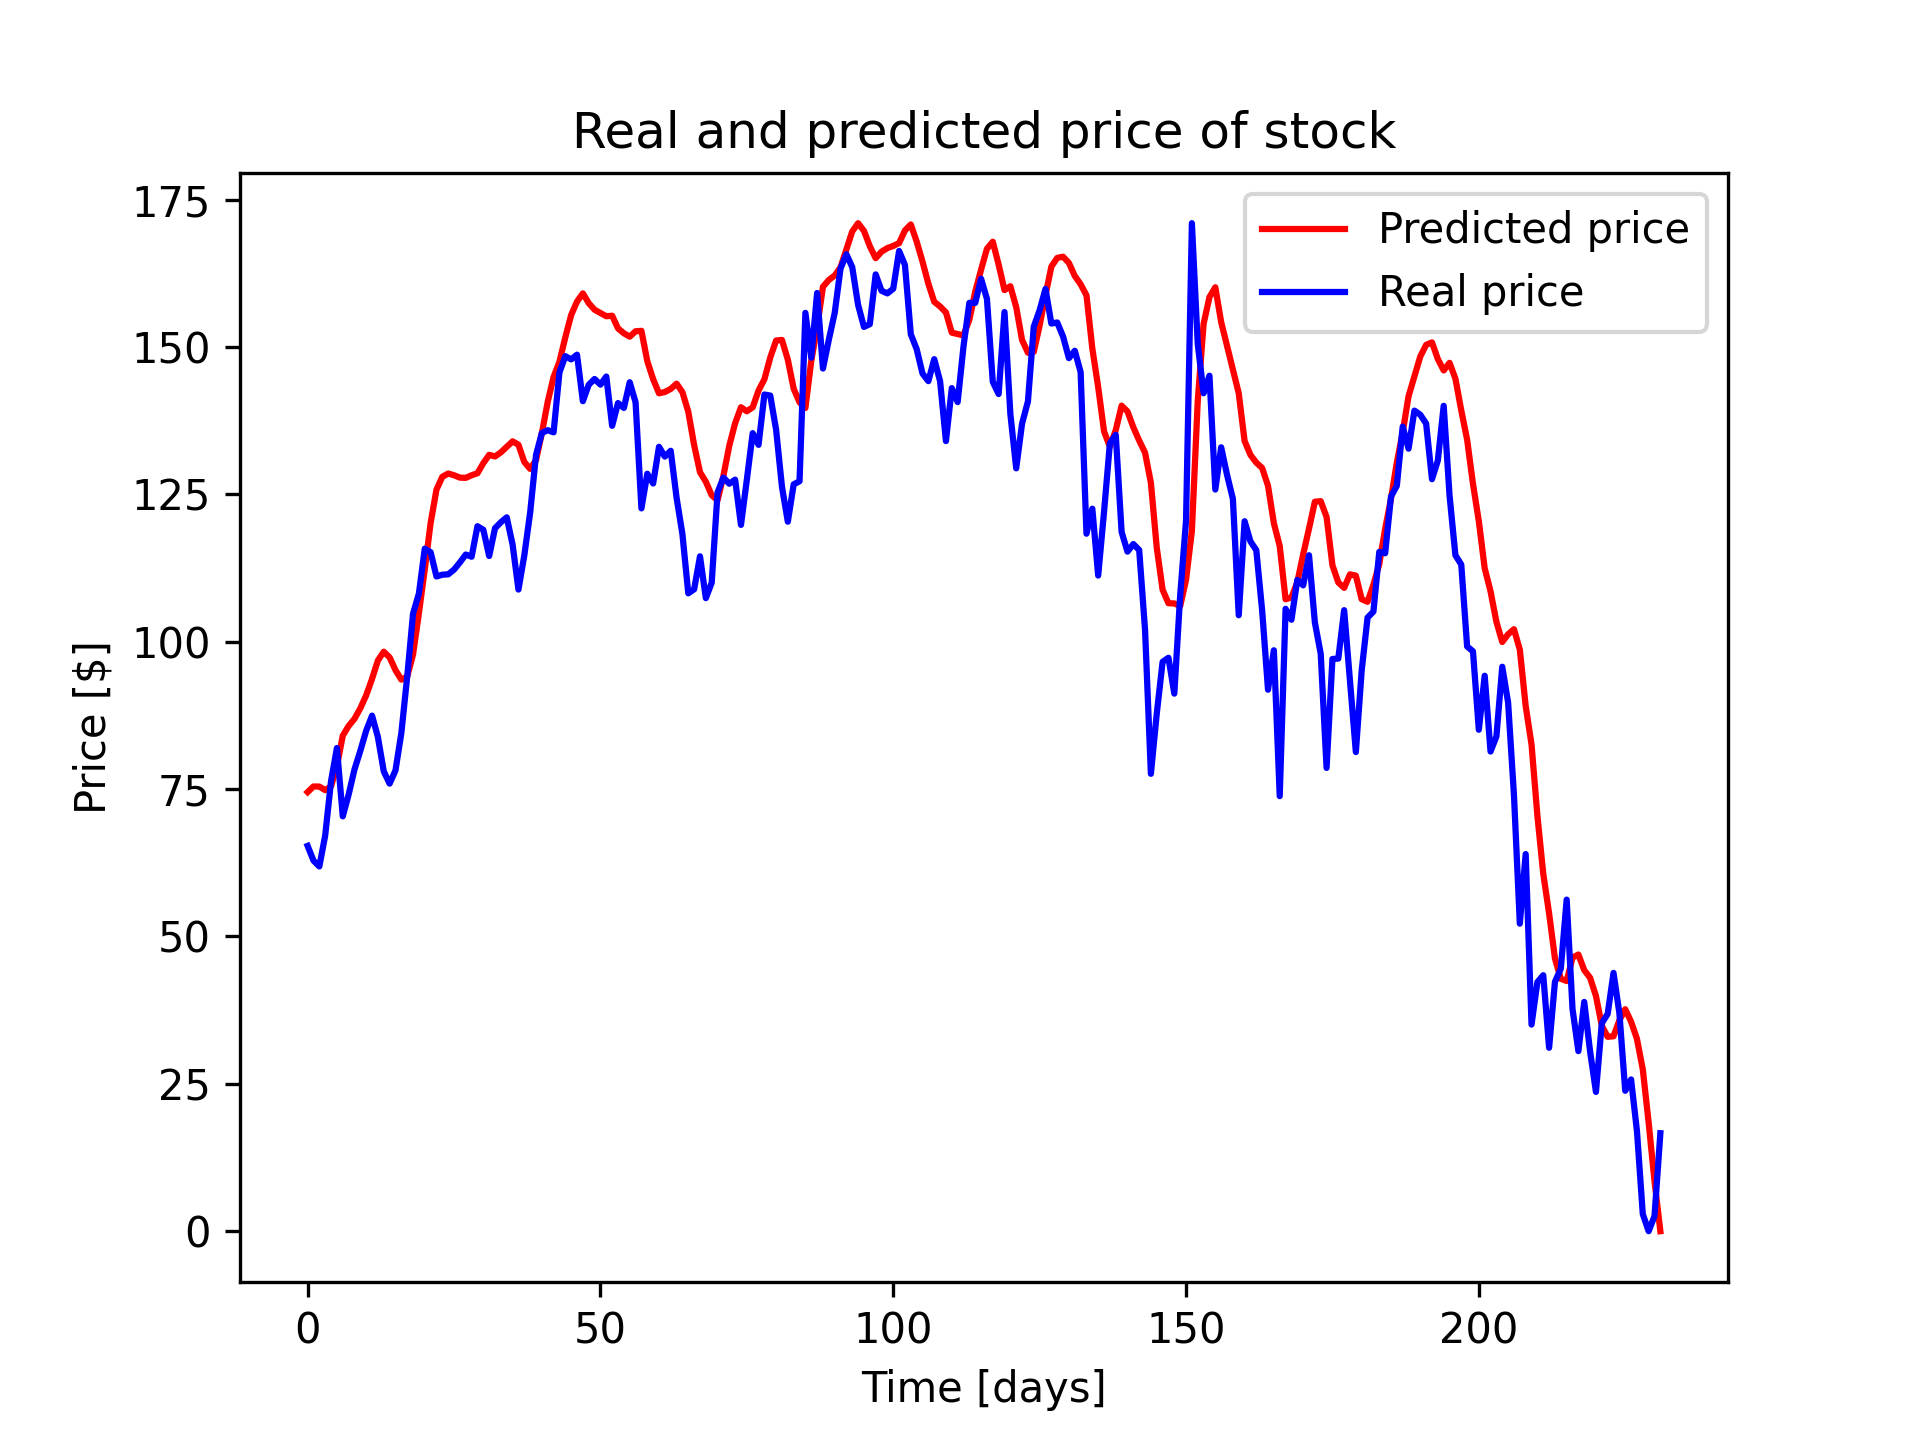
\includegraphics[width=0.5\textwidth]{./graf/model2/GOOGL.png}
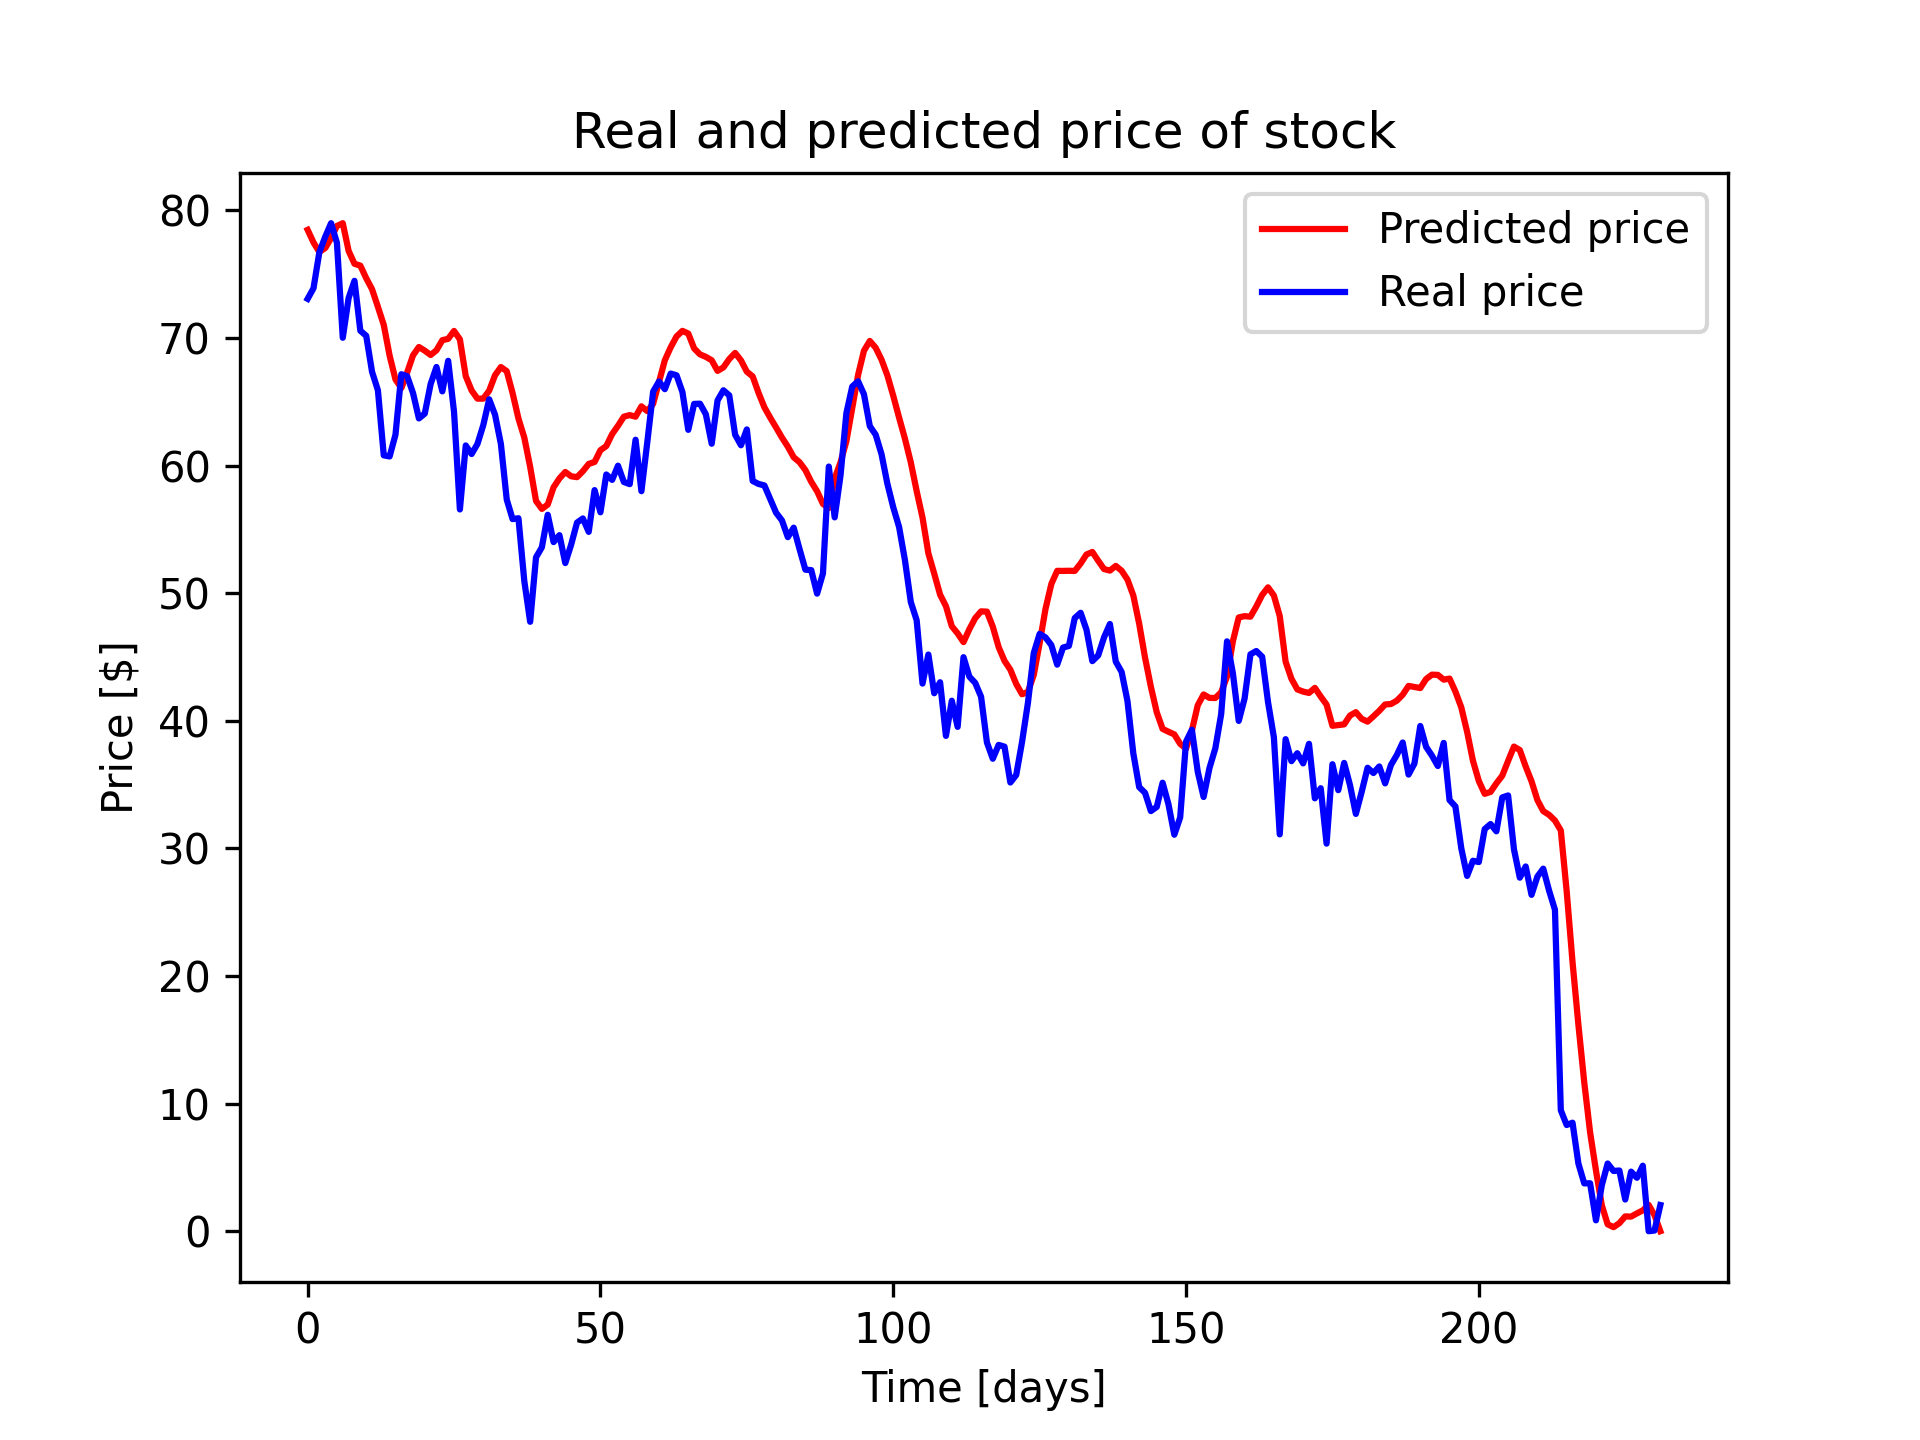
\includegraphics[width=0.5\textwidth]{./graf/model2/LYFT.png}
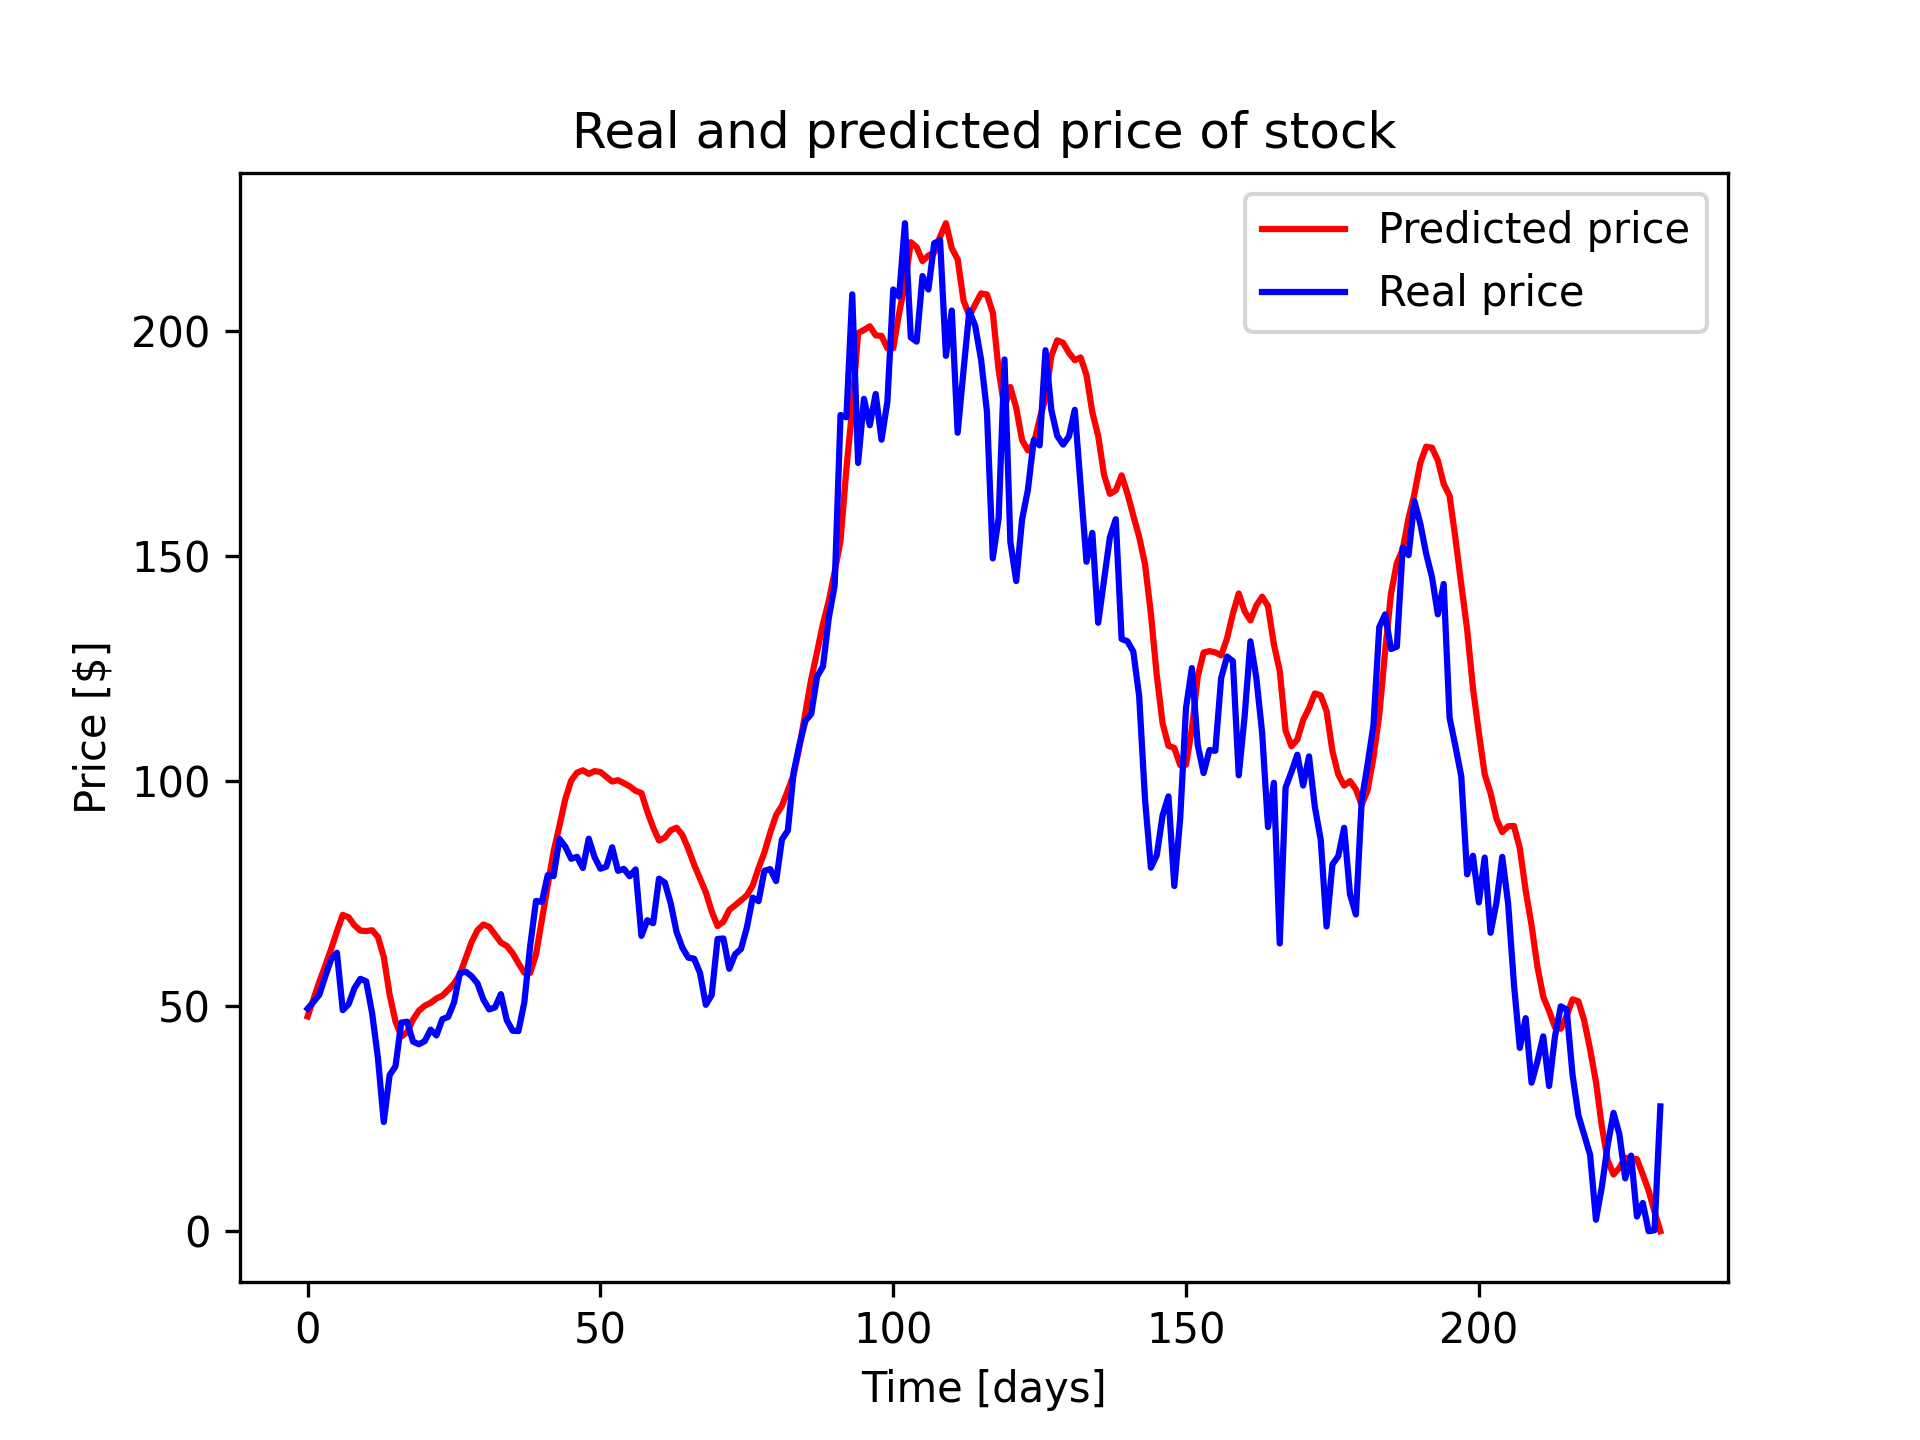
\includegraphics[width=0.5\textwidth]{./graf/model2/NVDA.png}
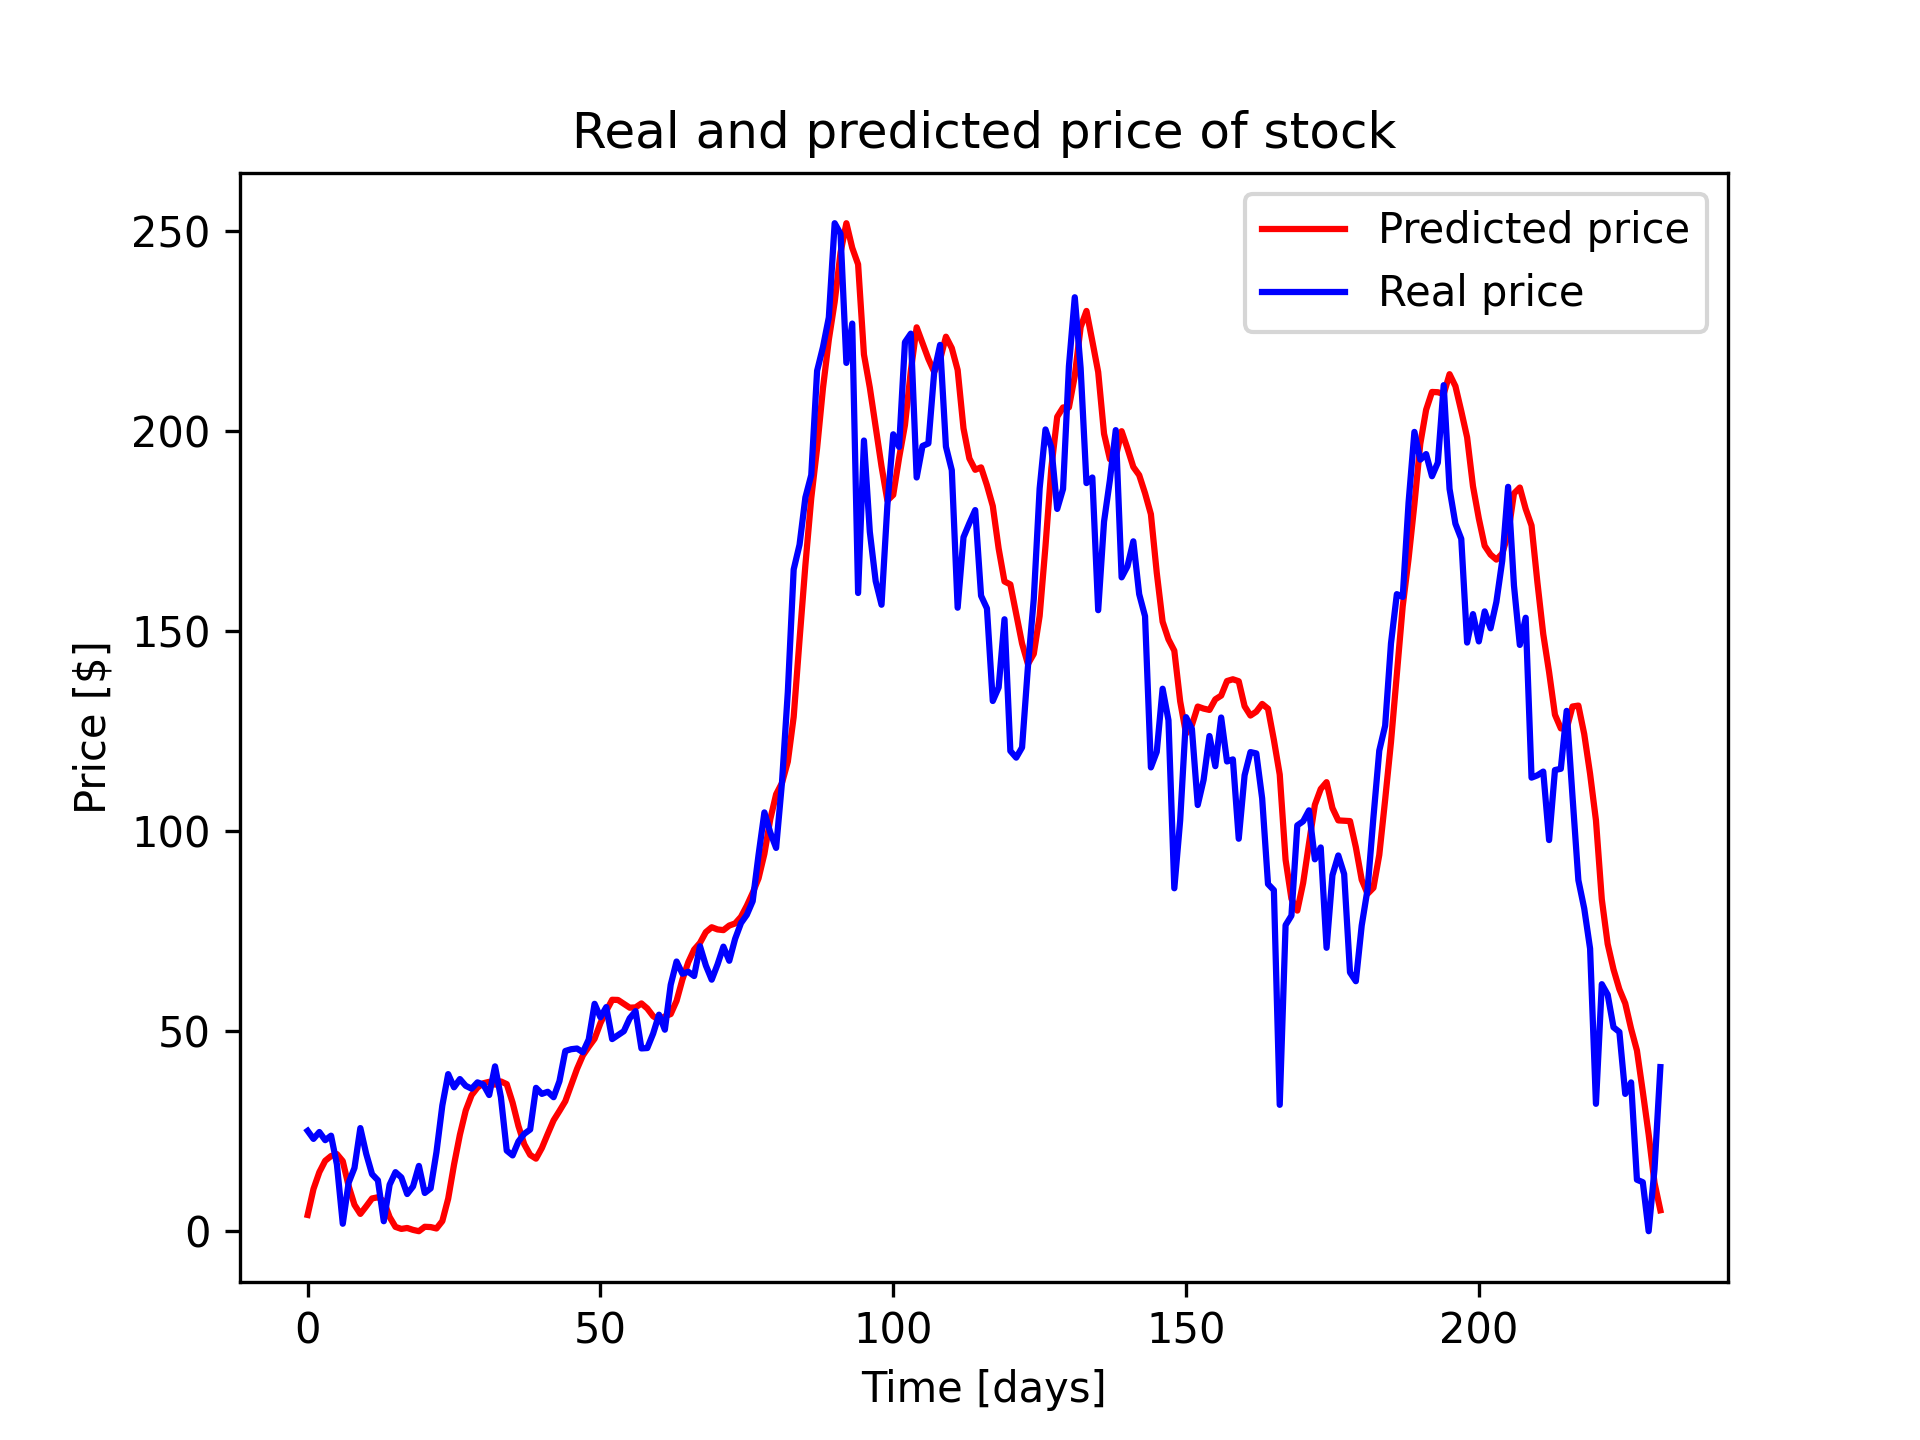
\includegraphics[width=0.5\textwidth]{./graf/model2/TSLA.png}
\caption{Real and predicted prices of the second model.}
\label{fig:label}
\end{figure} 

\clearpage
\subsection{Model 3}

Model3 - chunkSize: 20, time interval: 1 year, epochs: 15, trained on AAPL\par\bigskip
In the next model, at first glance, both lines almost coincide. After a careful analysis of the charts,
however, it can be seen that in some cases, the predicted price is slightly overestimated concerning
the real price. Some charts show that the predicted price is {\$}5 higher than the real price.
There are also visible lags of several days between the expected and real prices. In four plots
of this model (AAPL.png, GOOGL.png, NVDA.png, TSLA.png), it was observed that significant and
sudden amplitudes were not included in the sine of the red line.

\begin{figure}
% \centering
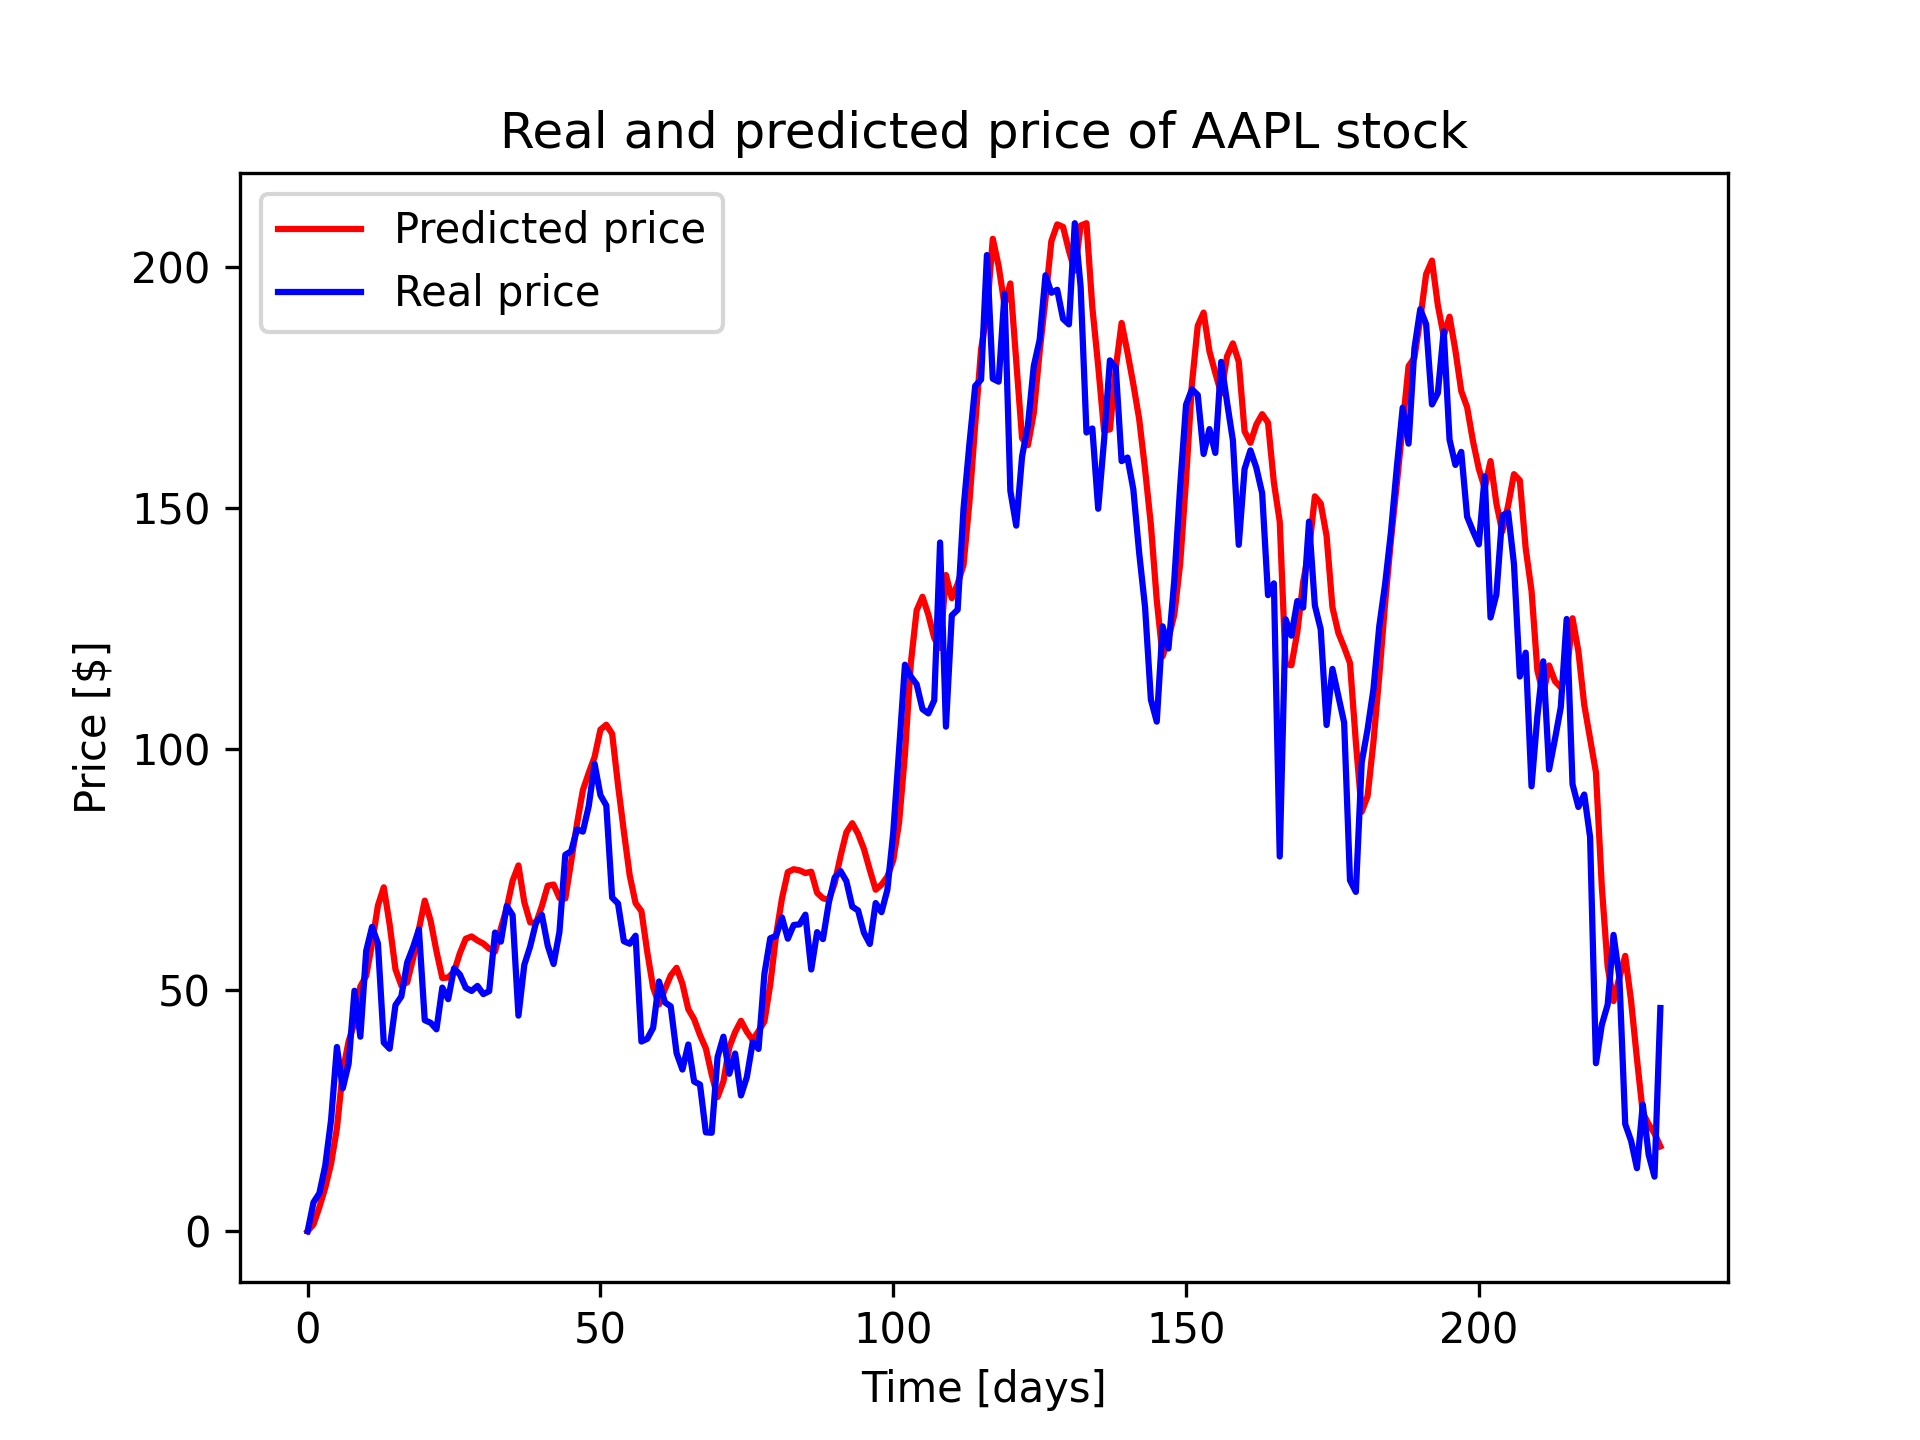
\includegraphics[width=0.5\textwidth]{./graf/model3/AAPL.png}
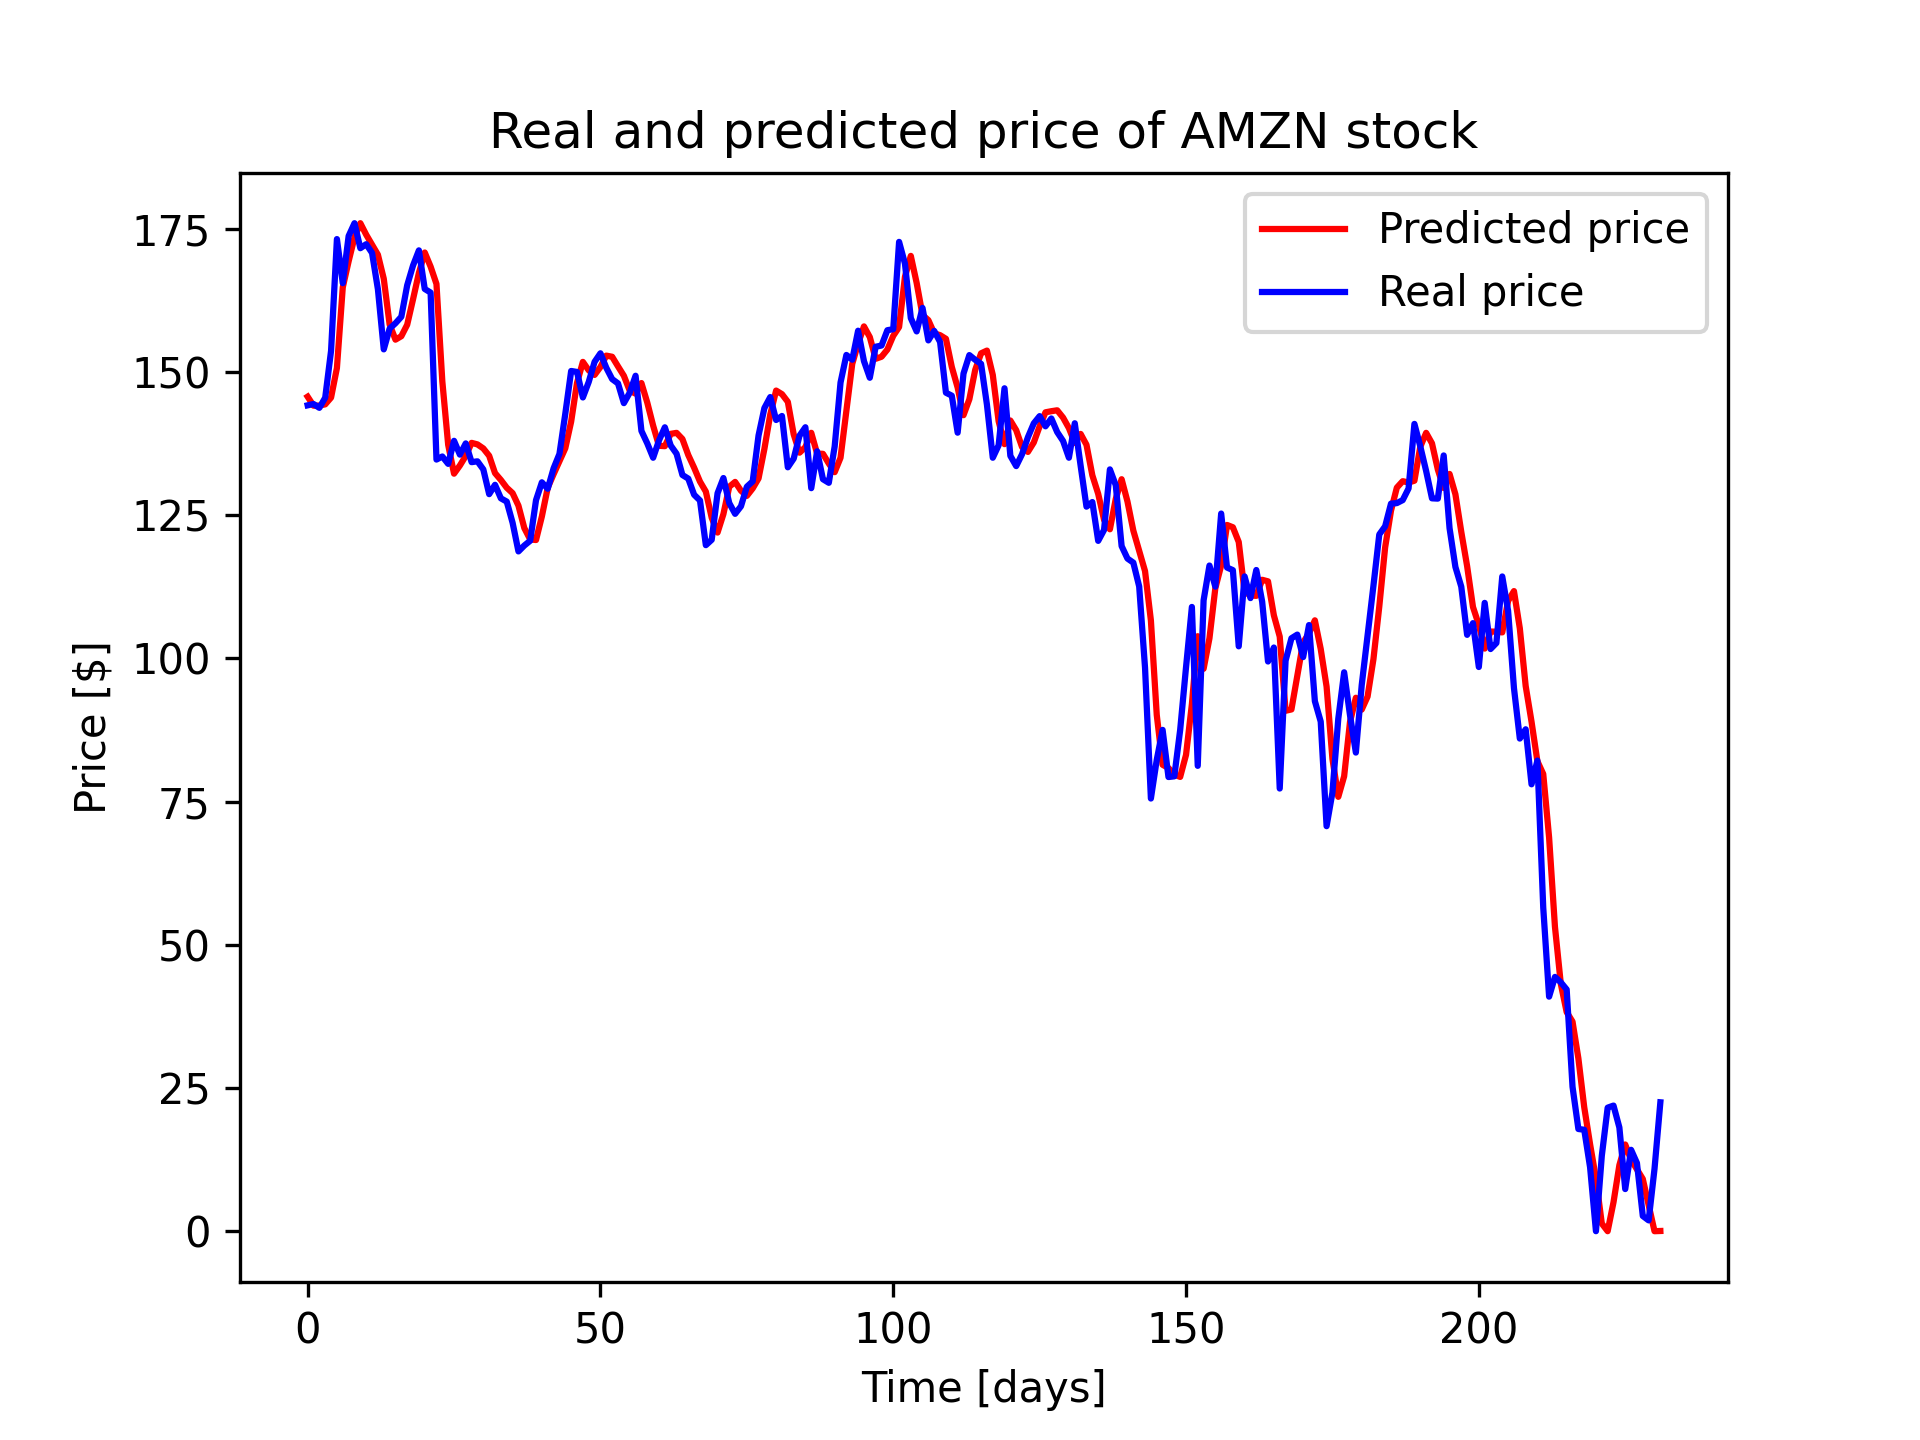
\includegraphics[width=0.5\textwidth]{./graf/model3/AMZN.png}
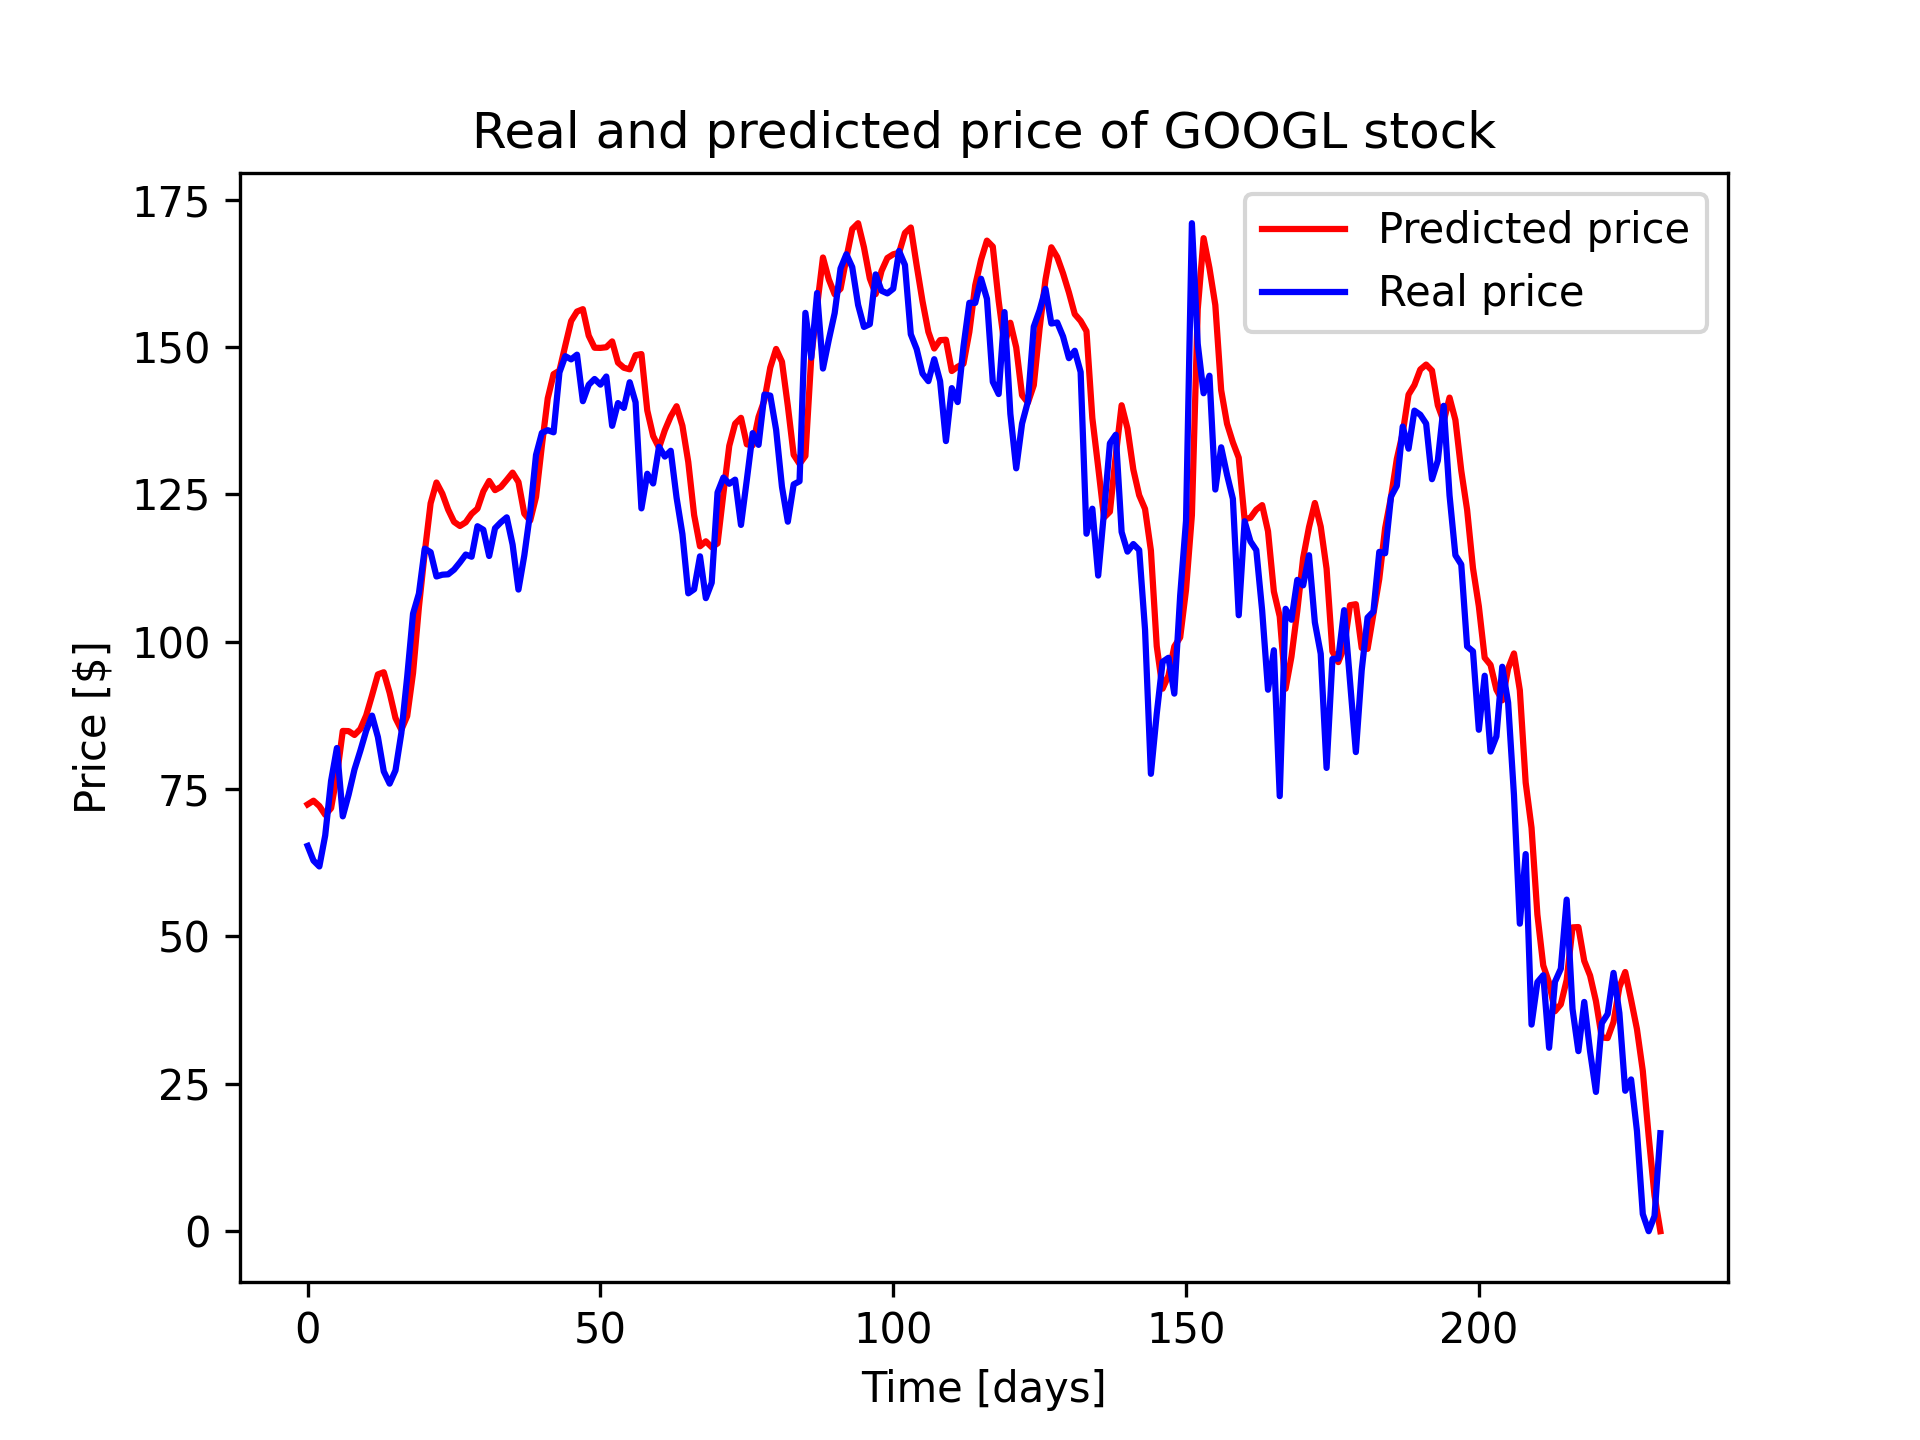
\includegraphics[width=0.5\textwidth]{./graf/model3/GOOGL.png}
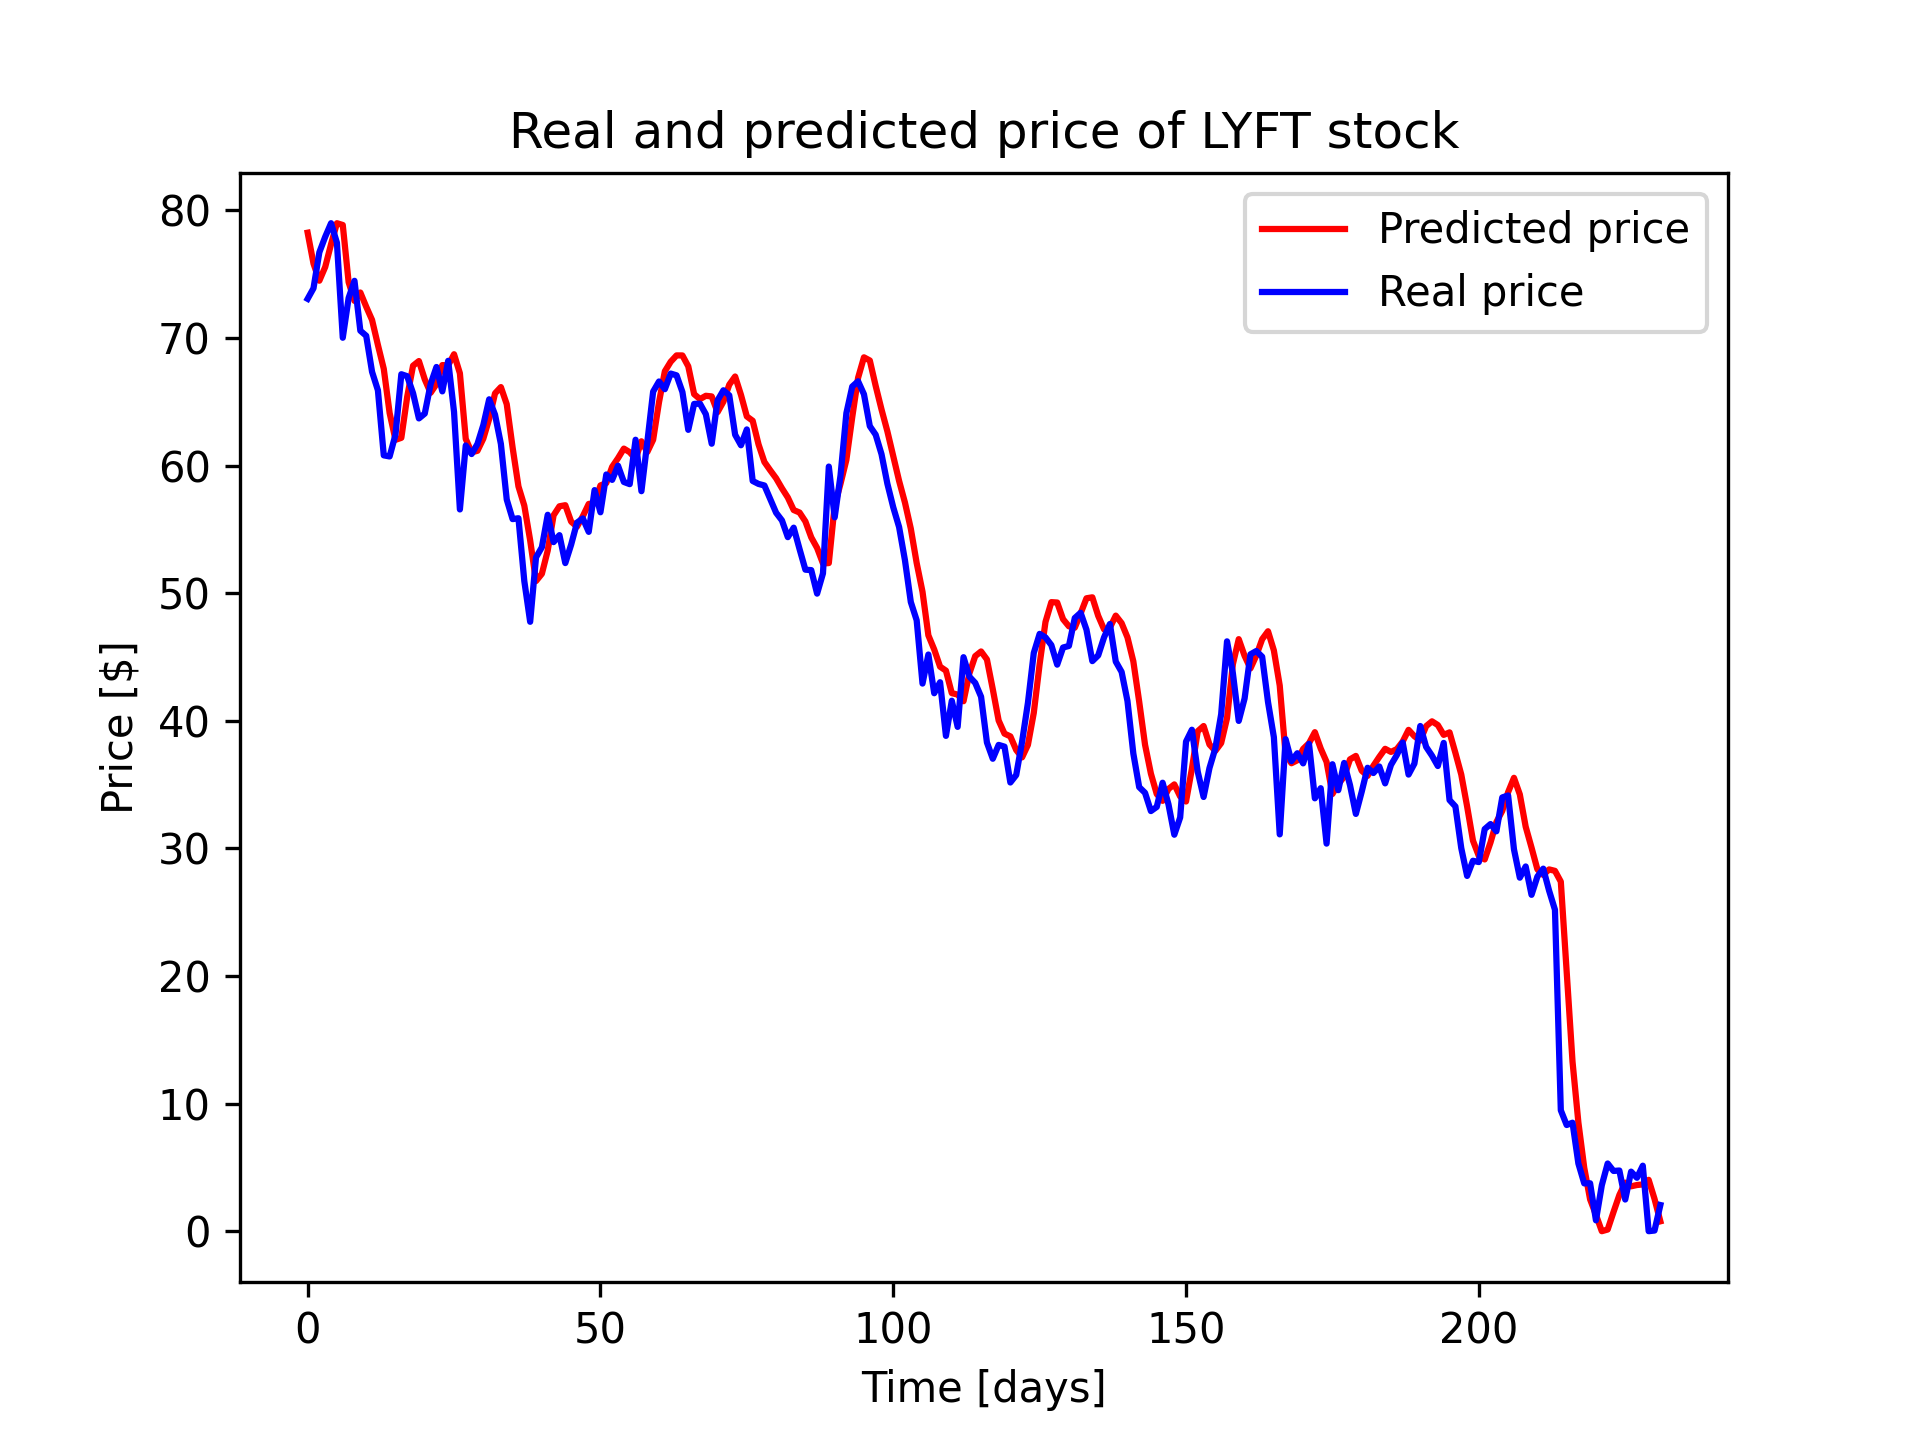
\includegraphics[width=0.5\textwidth]{./graf/model3/LYFT.png}
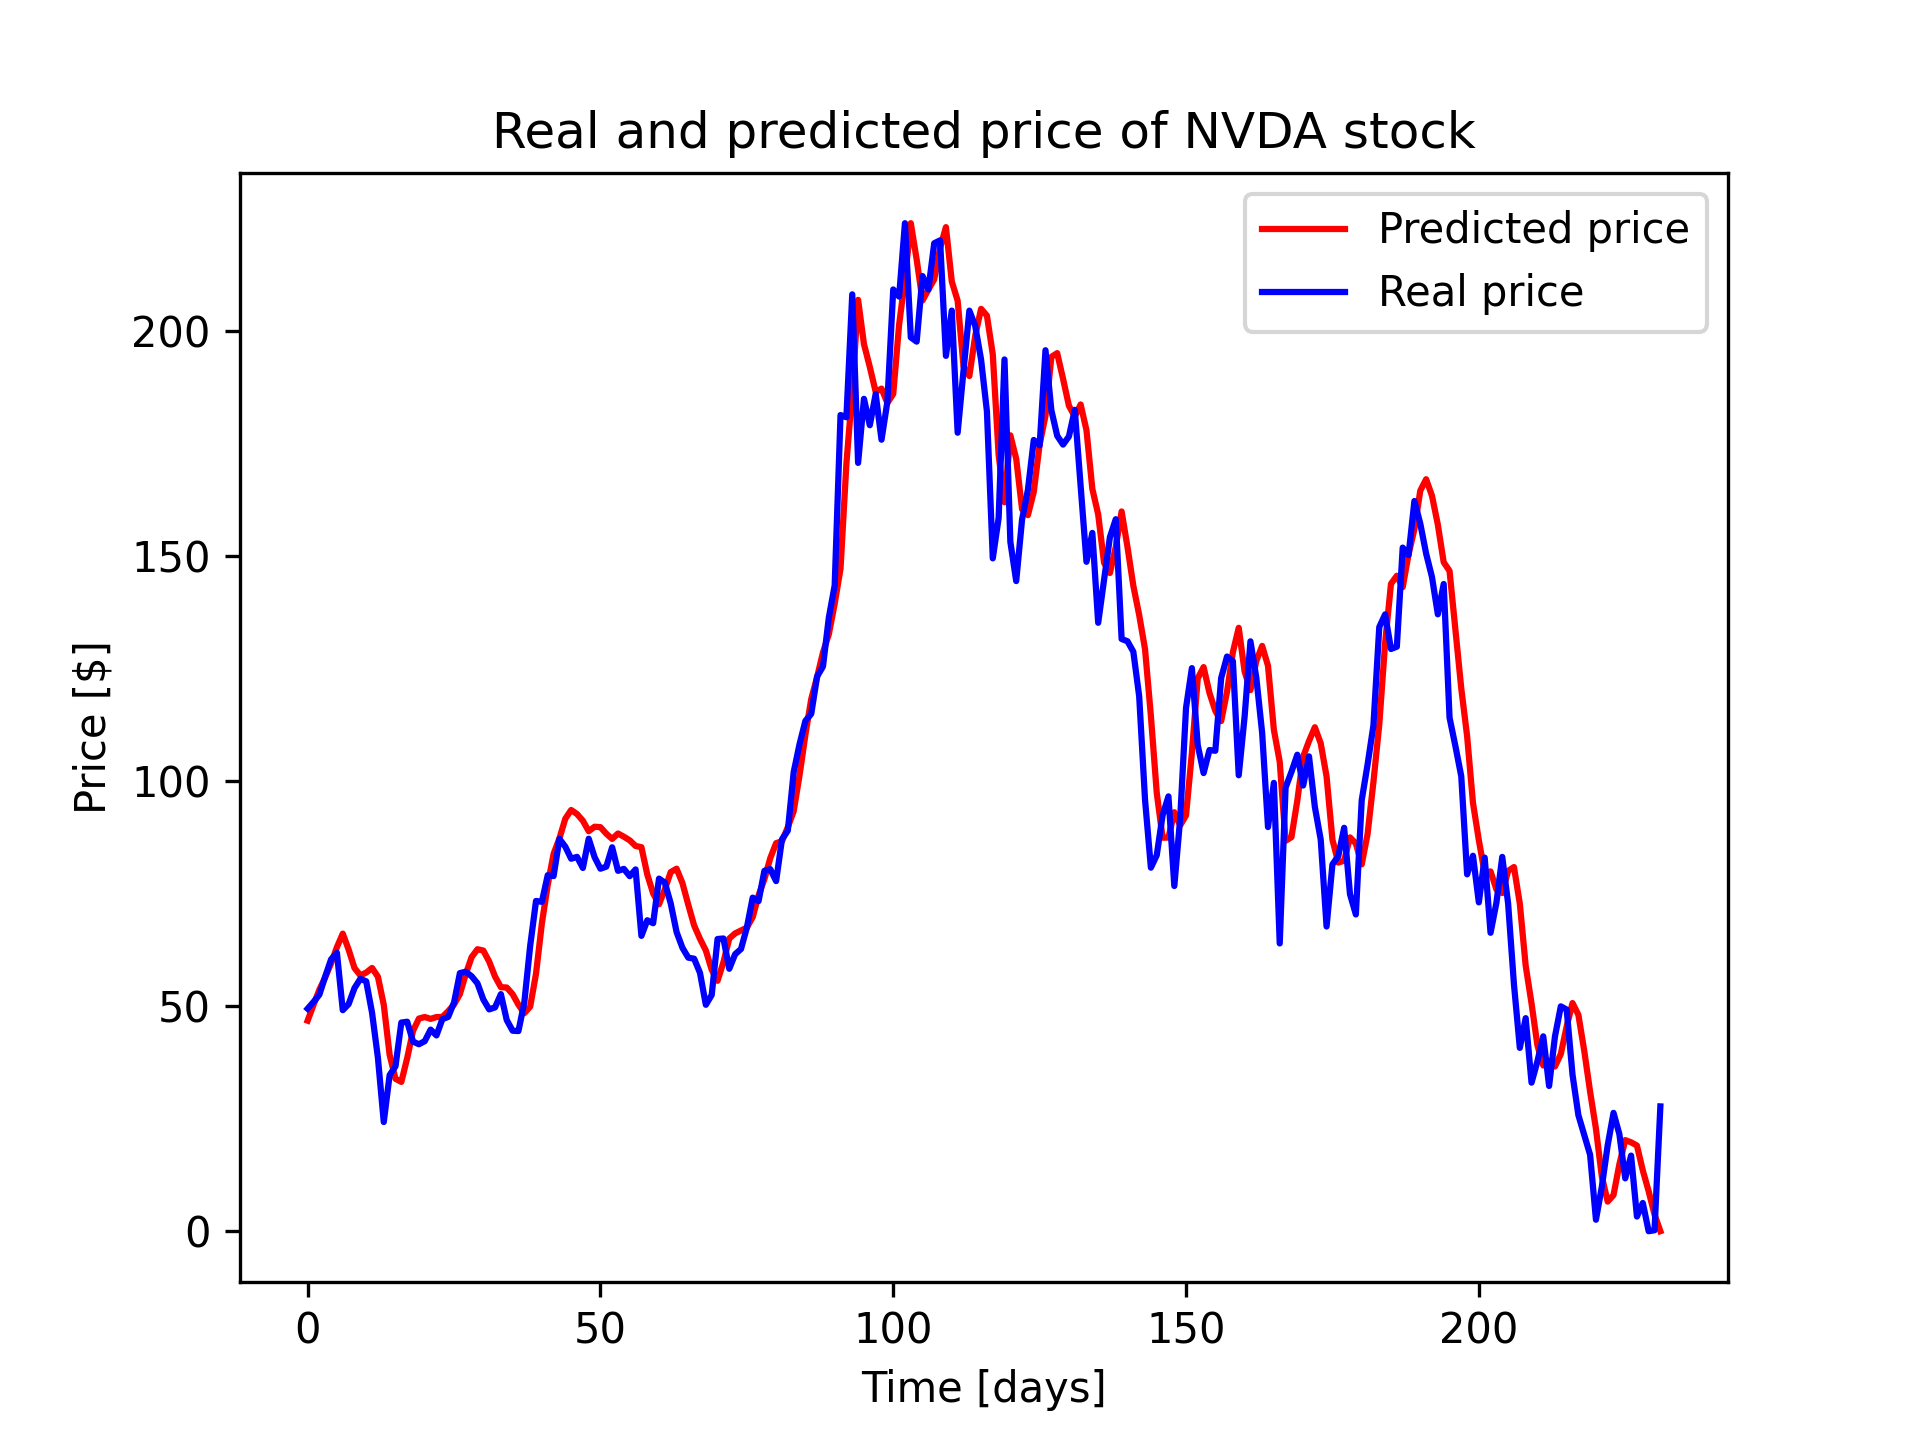
\includegraphics[width=0.5\textwidth]{./graf/model3/NVDA.png}
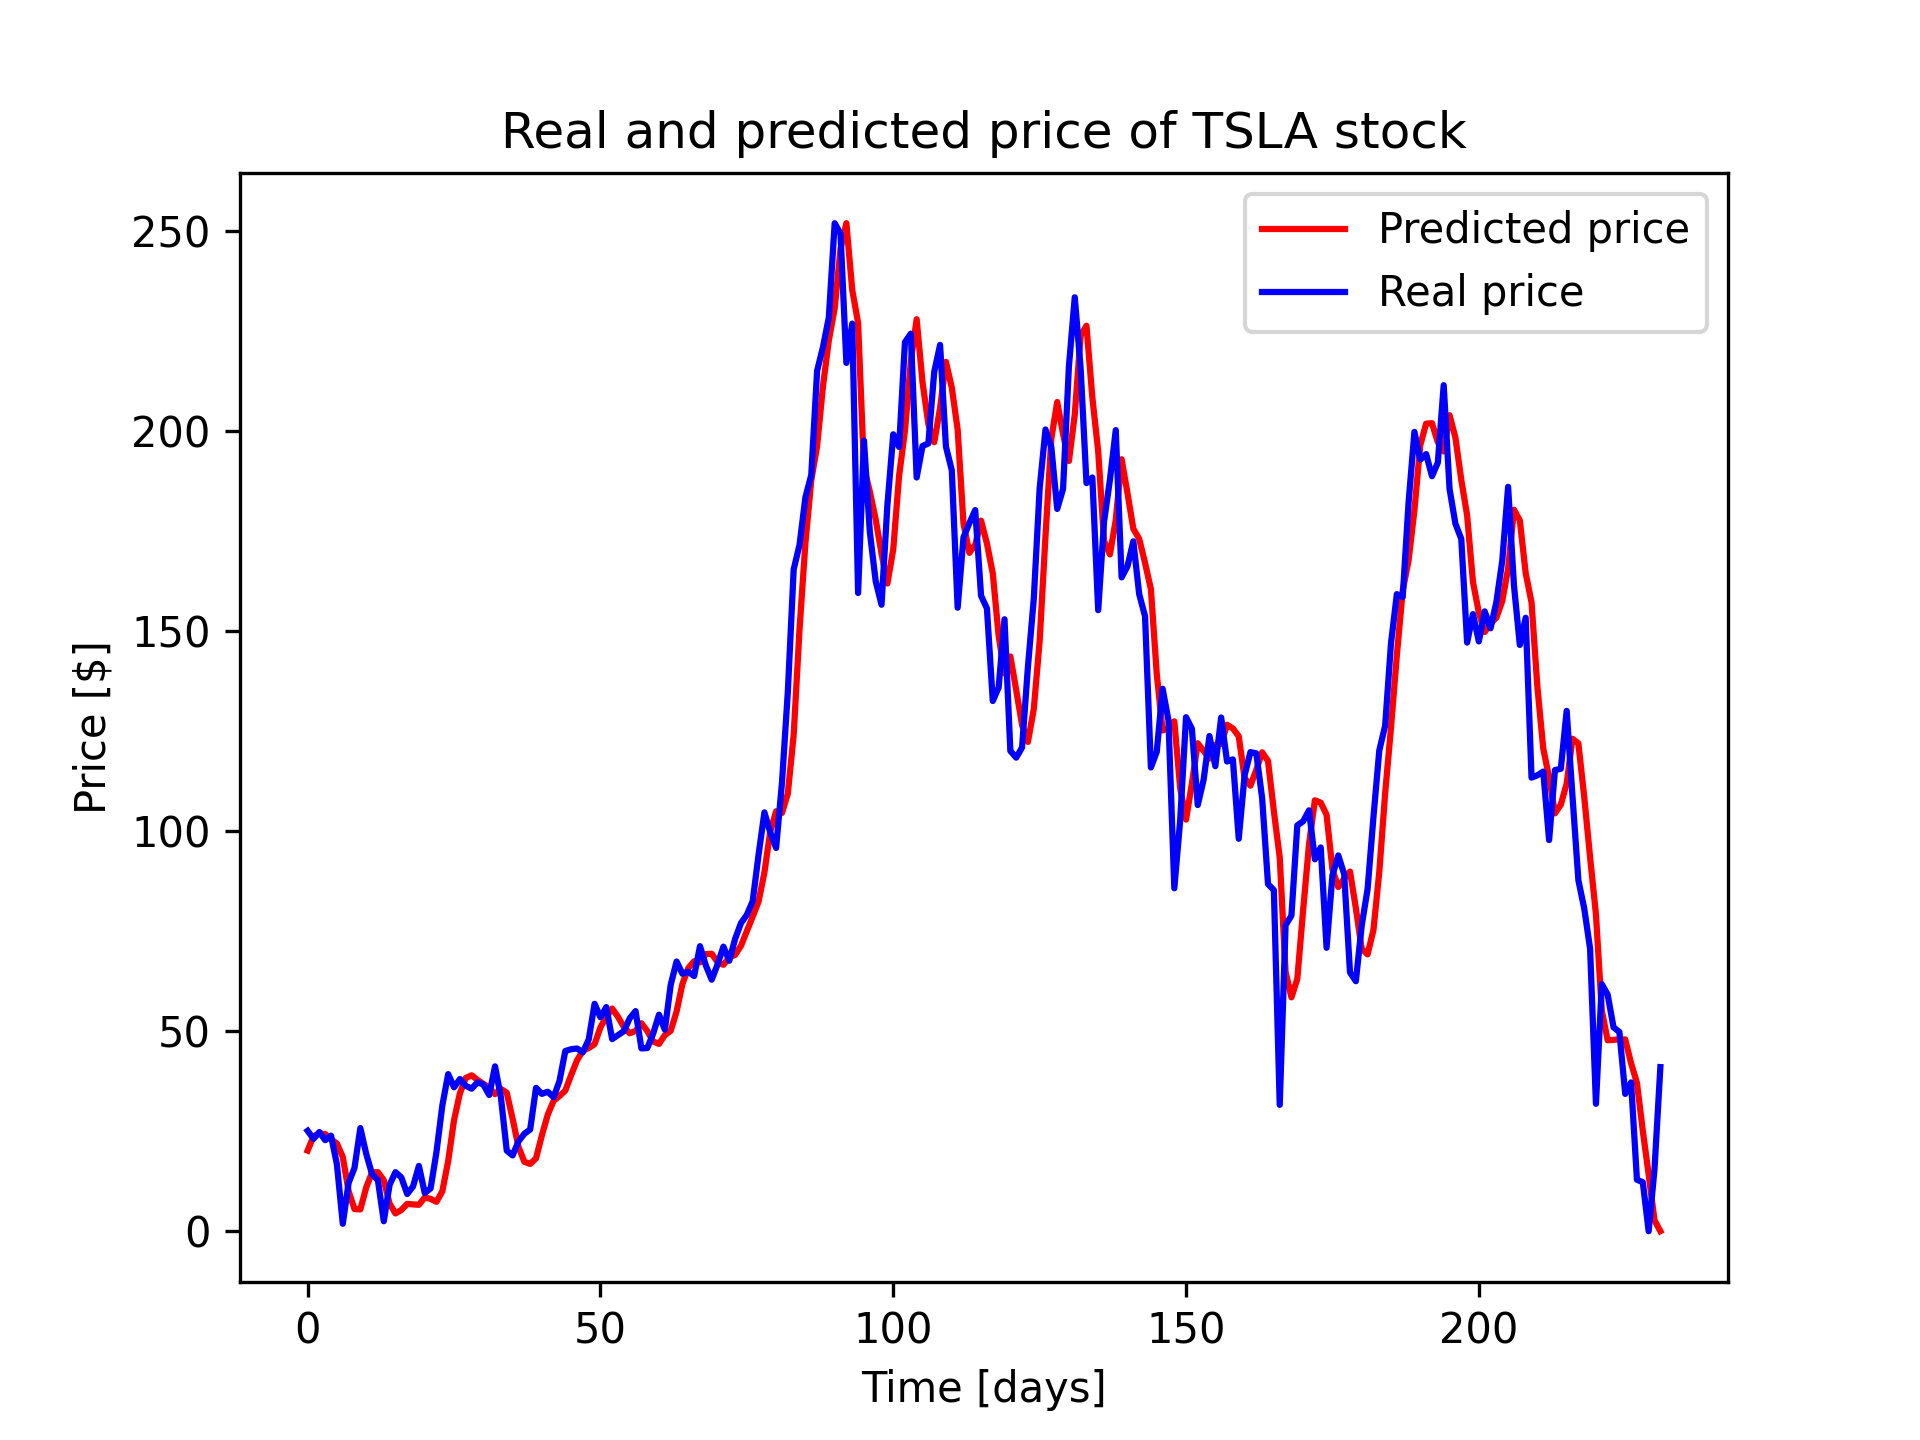
\includegraphics[width=0.5\textwidth]{./graf/model3/TSLA.png}
\caption{Real and predicted prices of the third model.}
\label{fig:label}
\end{figure} 

\clearpage
\subsection{Model 4}

Model4 - chunkSize: 50, time interval: 1 year, epochs: 5, trained on AAPL\par\bigskip
Analyzing model 4 in terms of the convergence of the predicted price to the real price, it can be seen that in places where the amplitude swings sharply, there are discrepancies in the course of
both lines relative to each other. In the AMZN.png and LYFT.png charts, the red line runs slightly
ahead of the real price line and is slightly above it. In the remaining charts, there is a tendency for
both lines to intersect in several areas. The red line shows short-term price fluctuations in minor
detail, showing only the general direction of the downward or upward trend.

\begin{figure}
% \centering
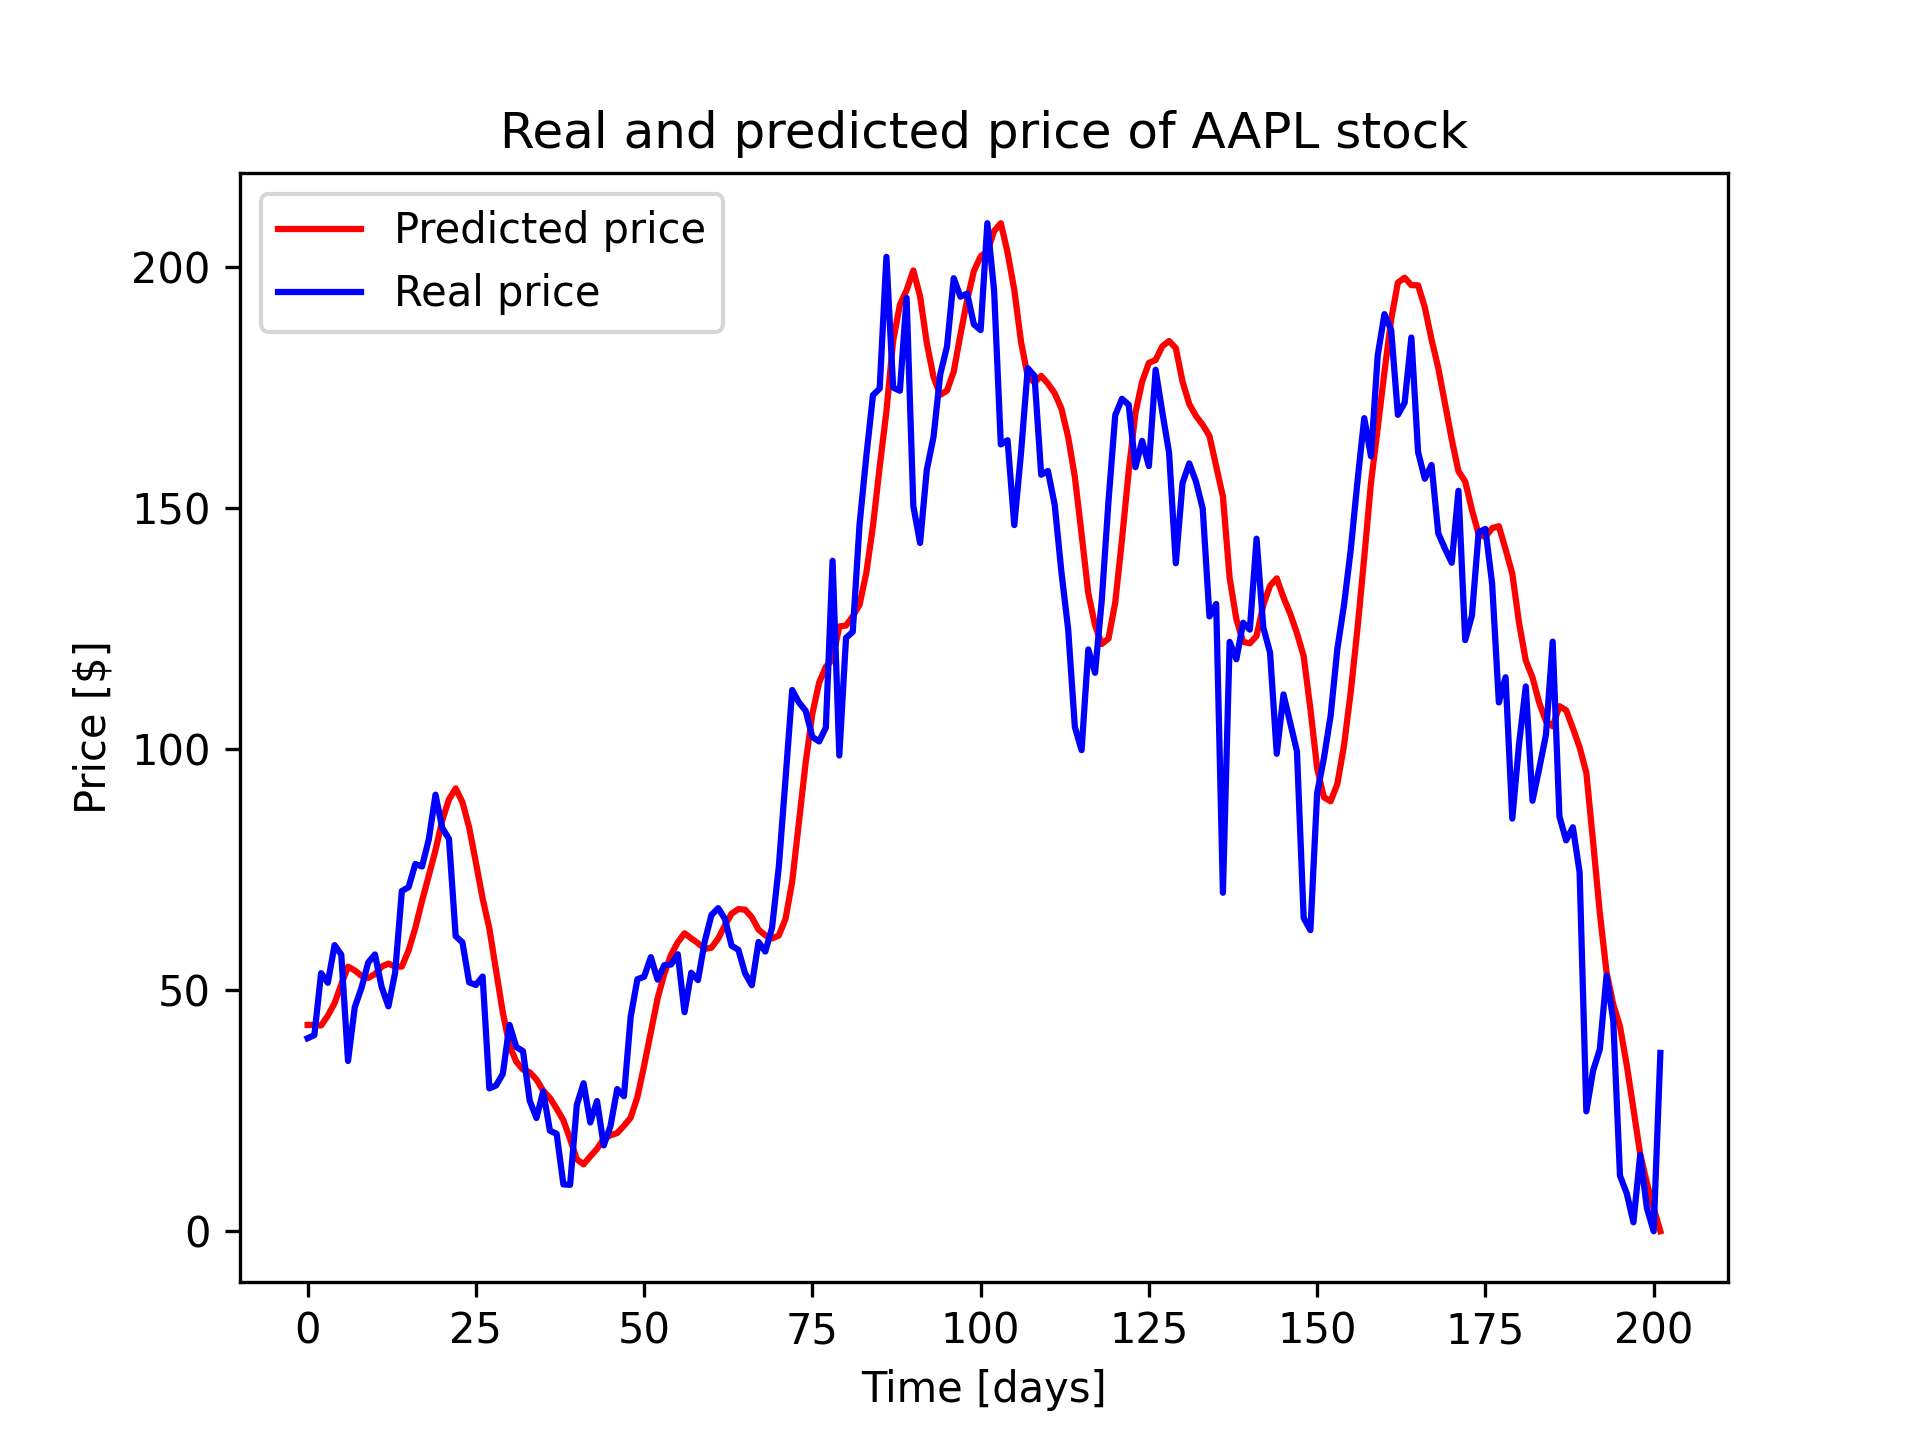
\includegraphics[width=0.5\textwidth]{./graf/model4/AAPL.png}
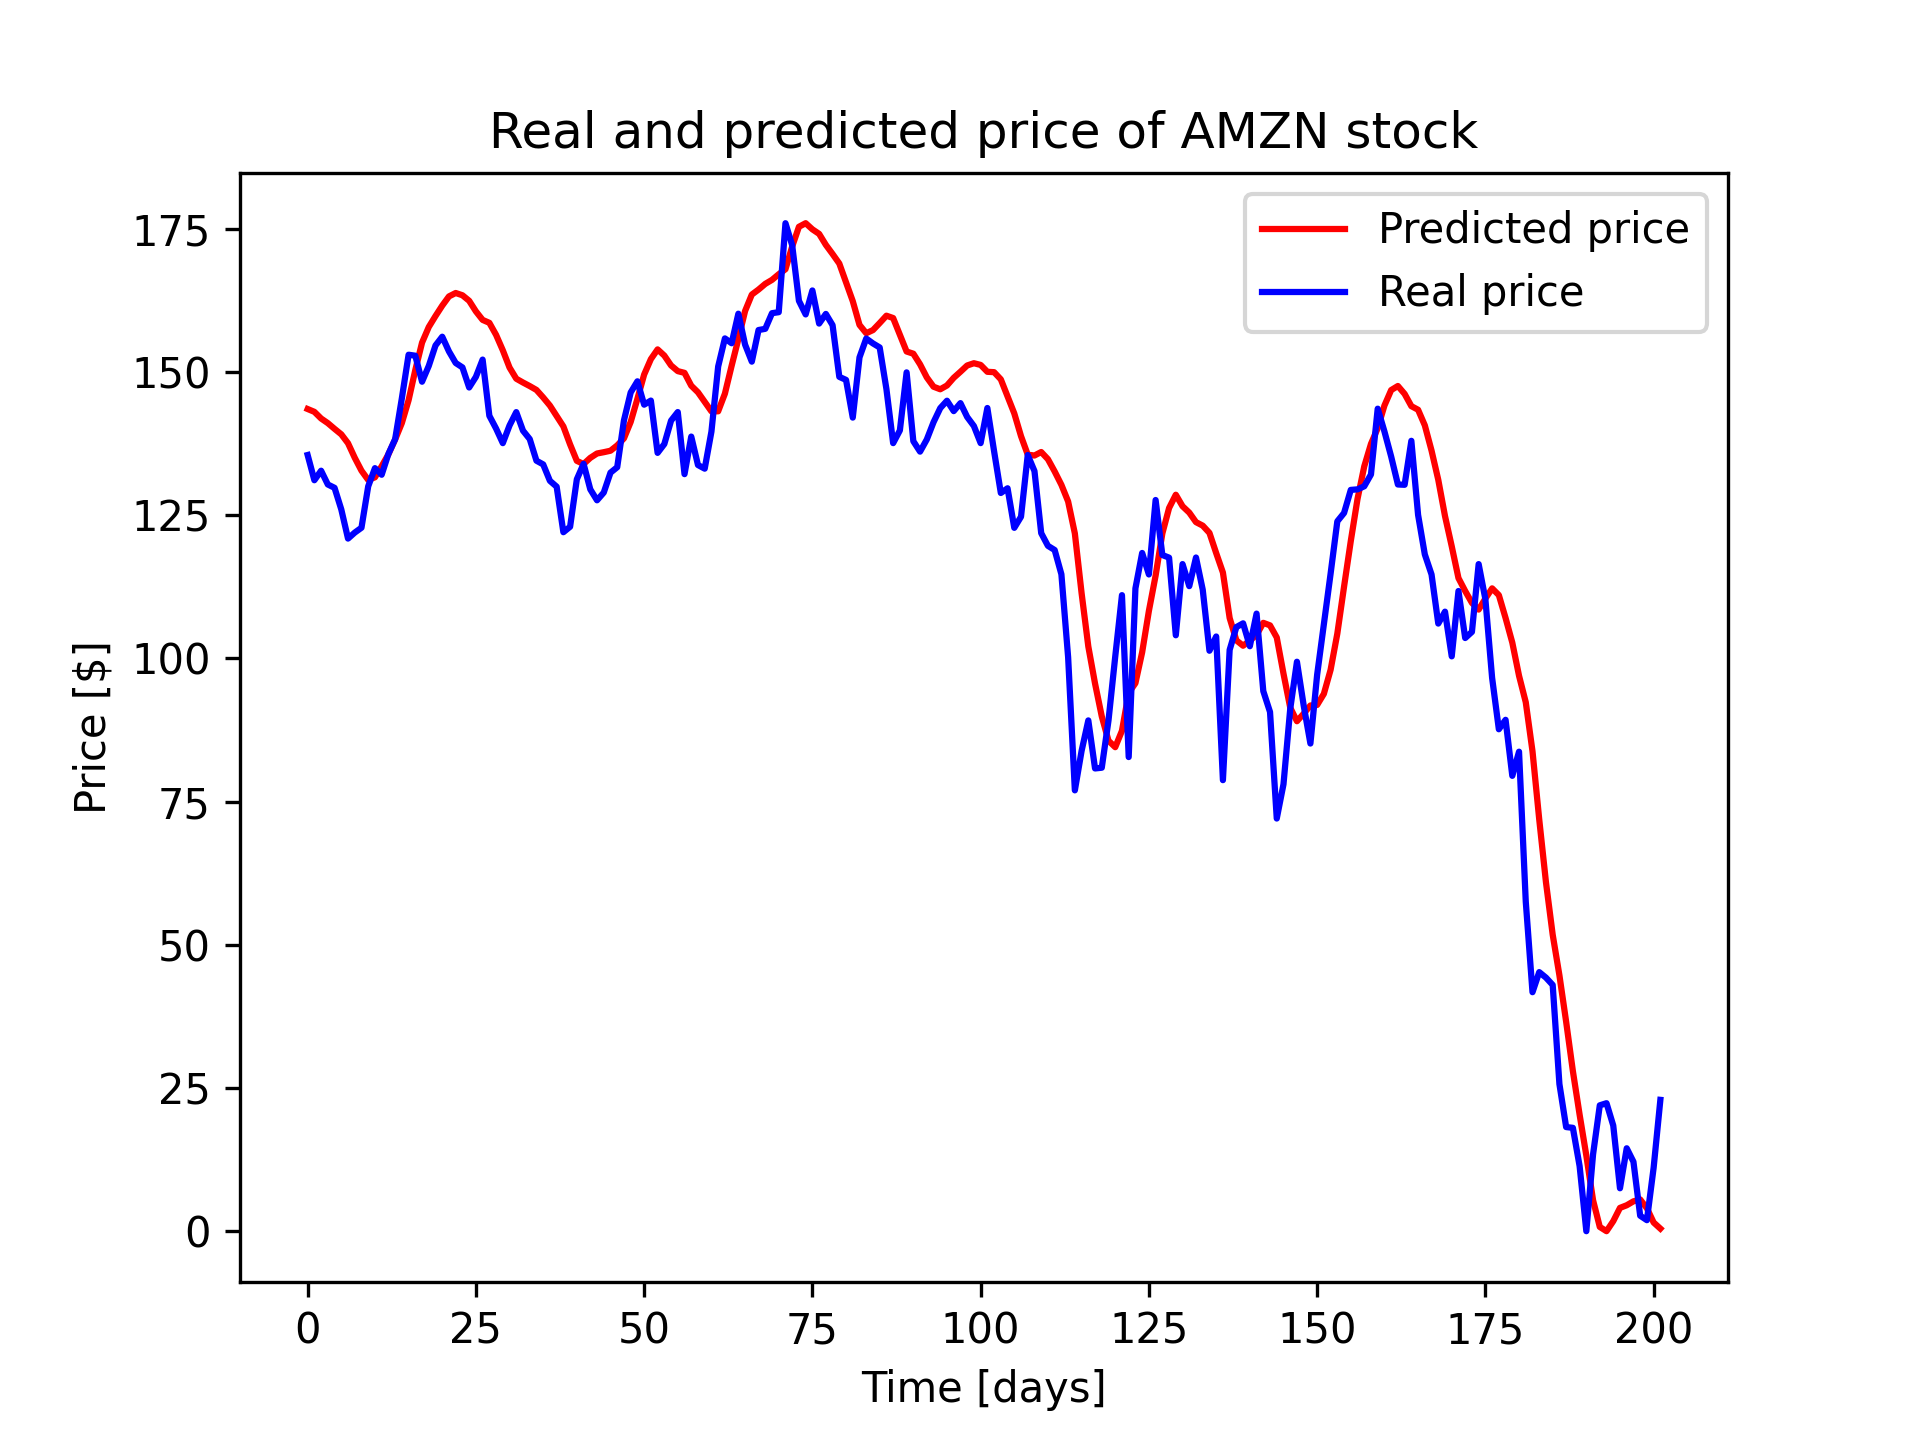
\includegraphics[width=0.5\textwidth]{./graf/model4/AMZN.png}
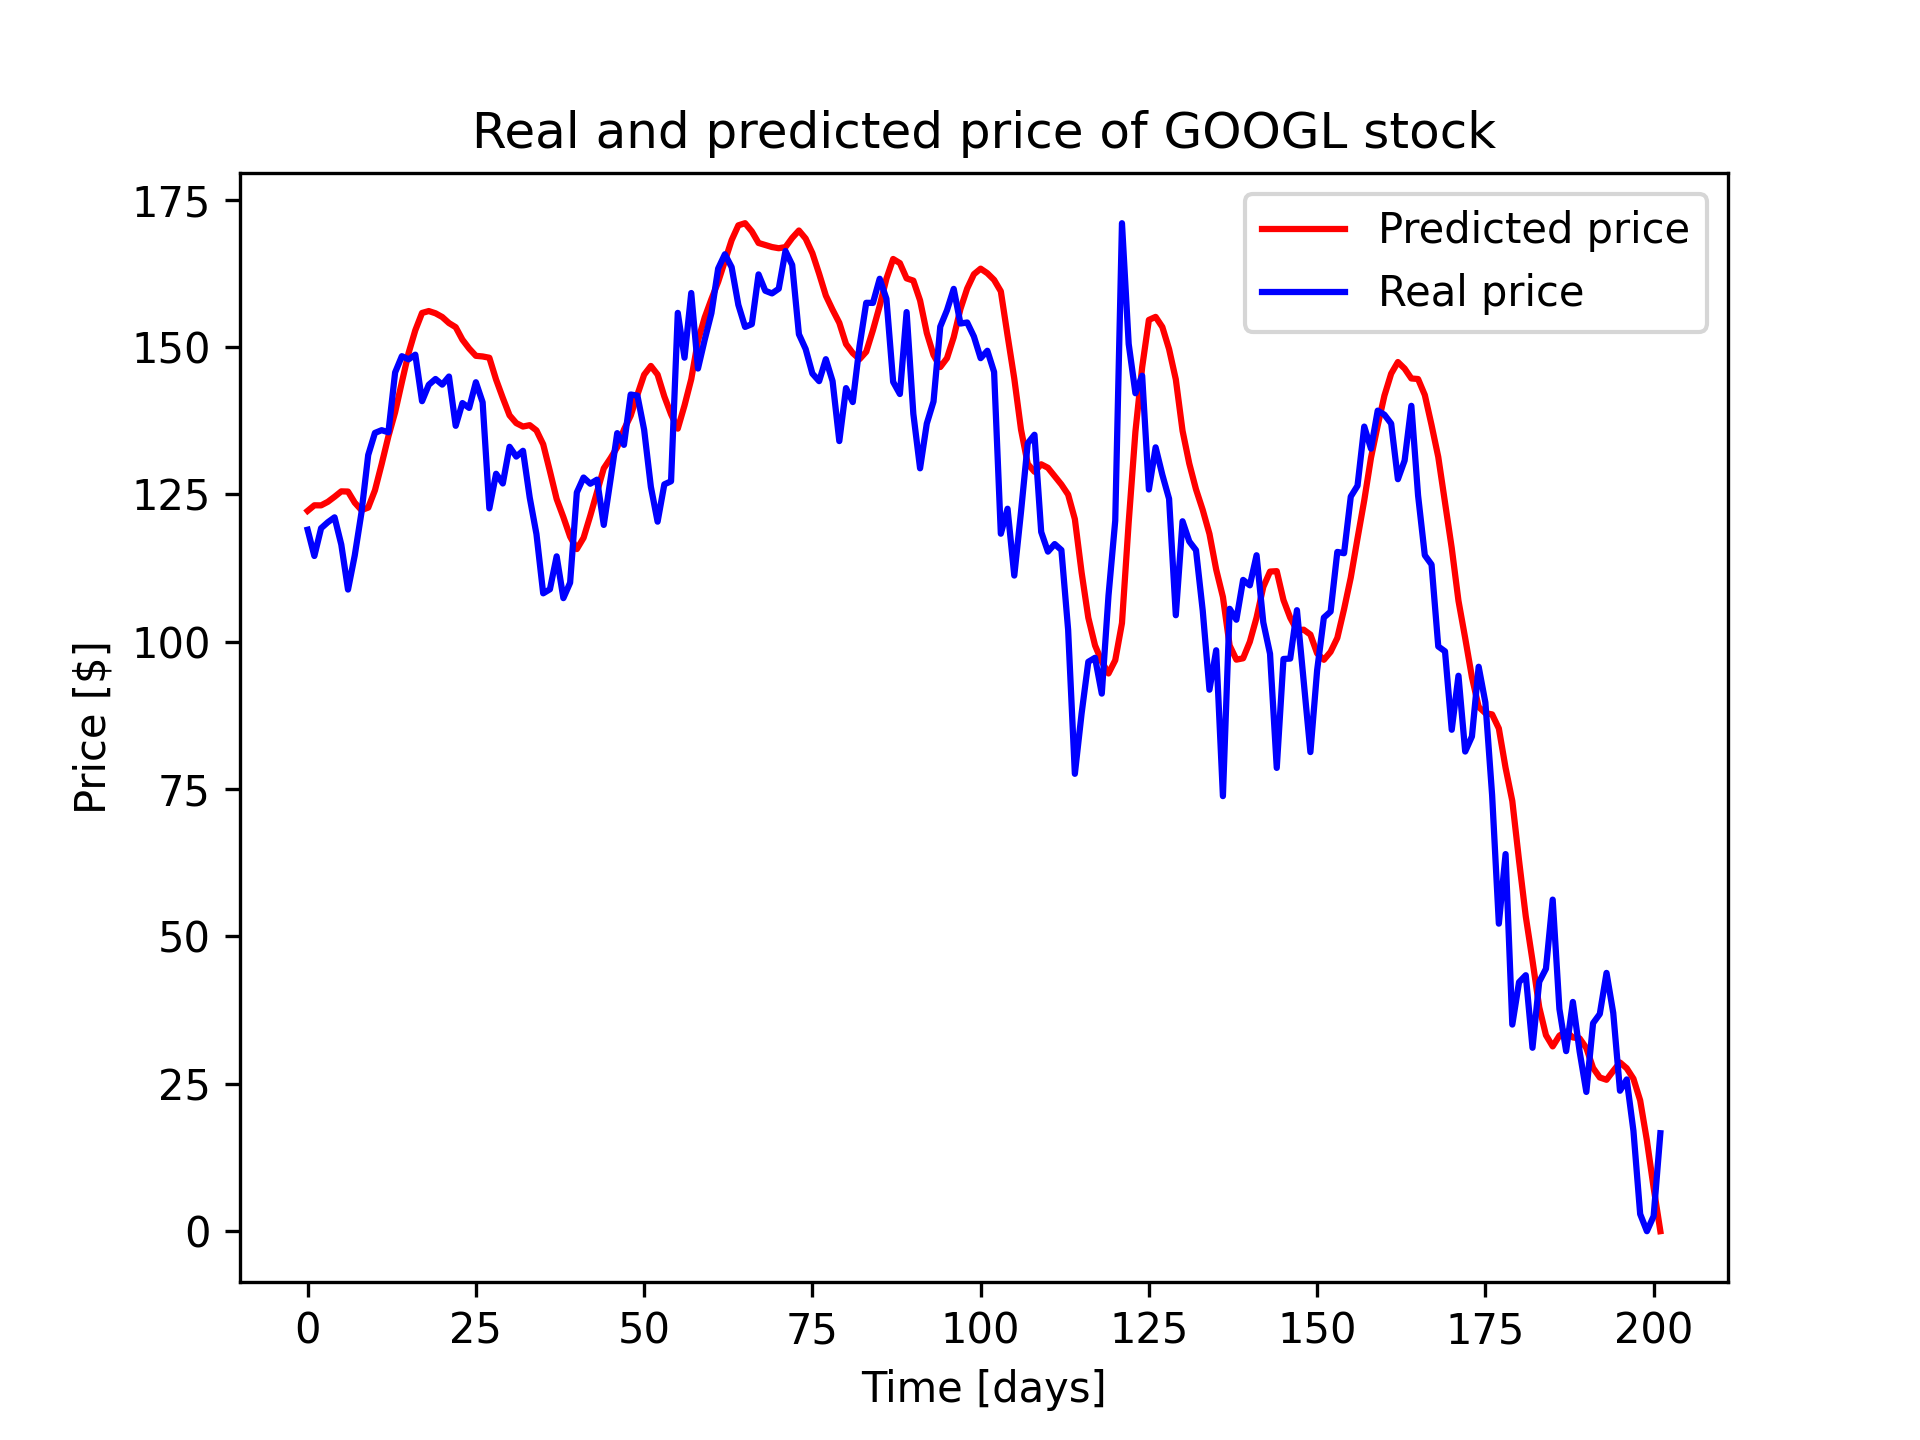
\includegraphics[width=0.5\textwidth]{./graf/model4/GOOGL.png}
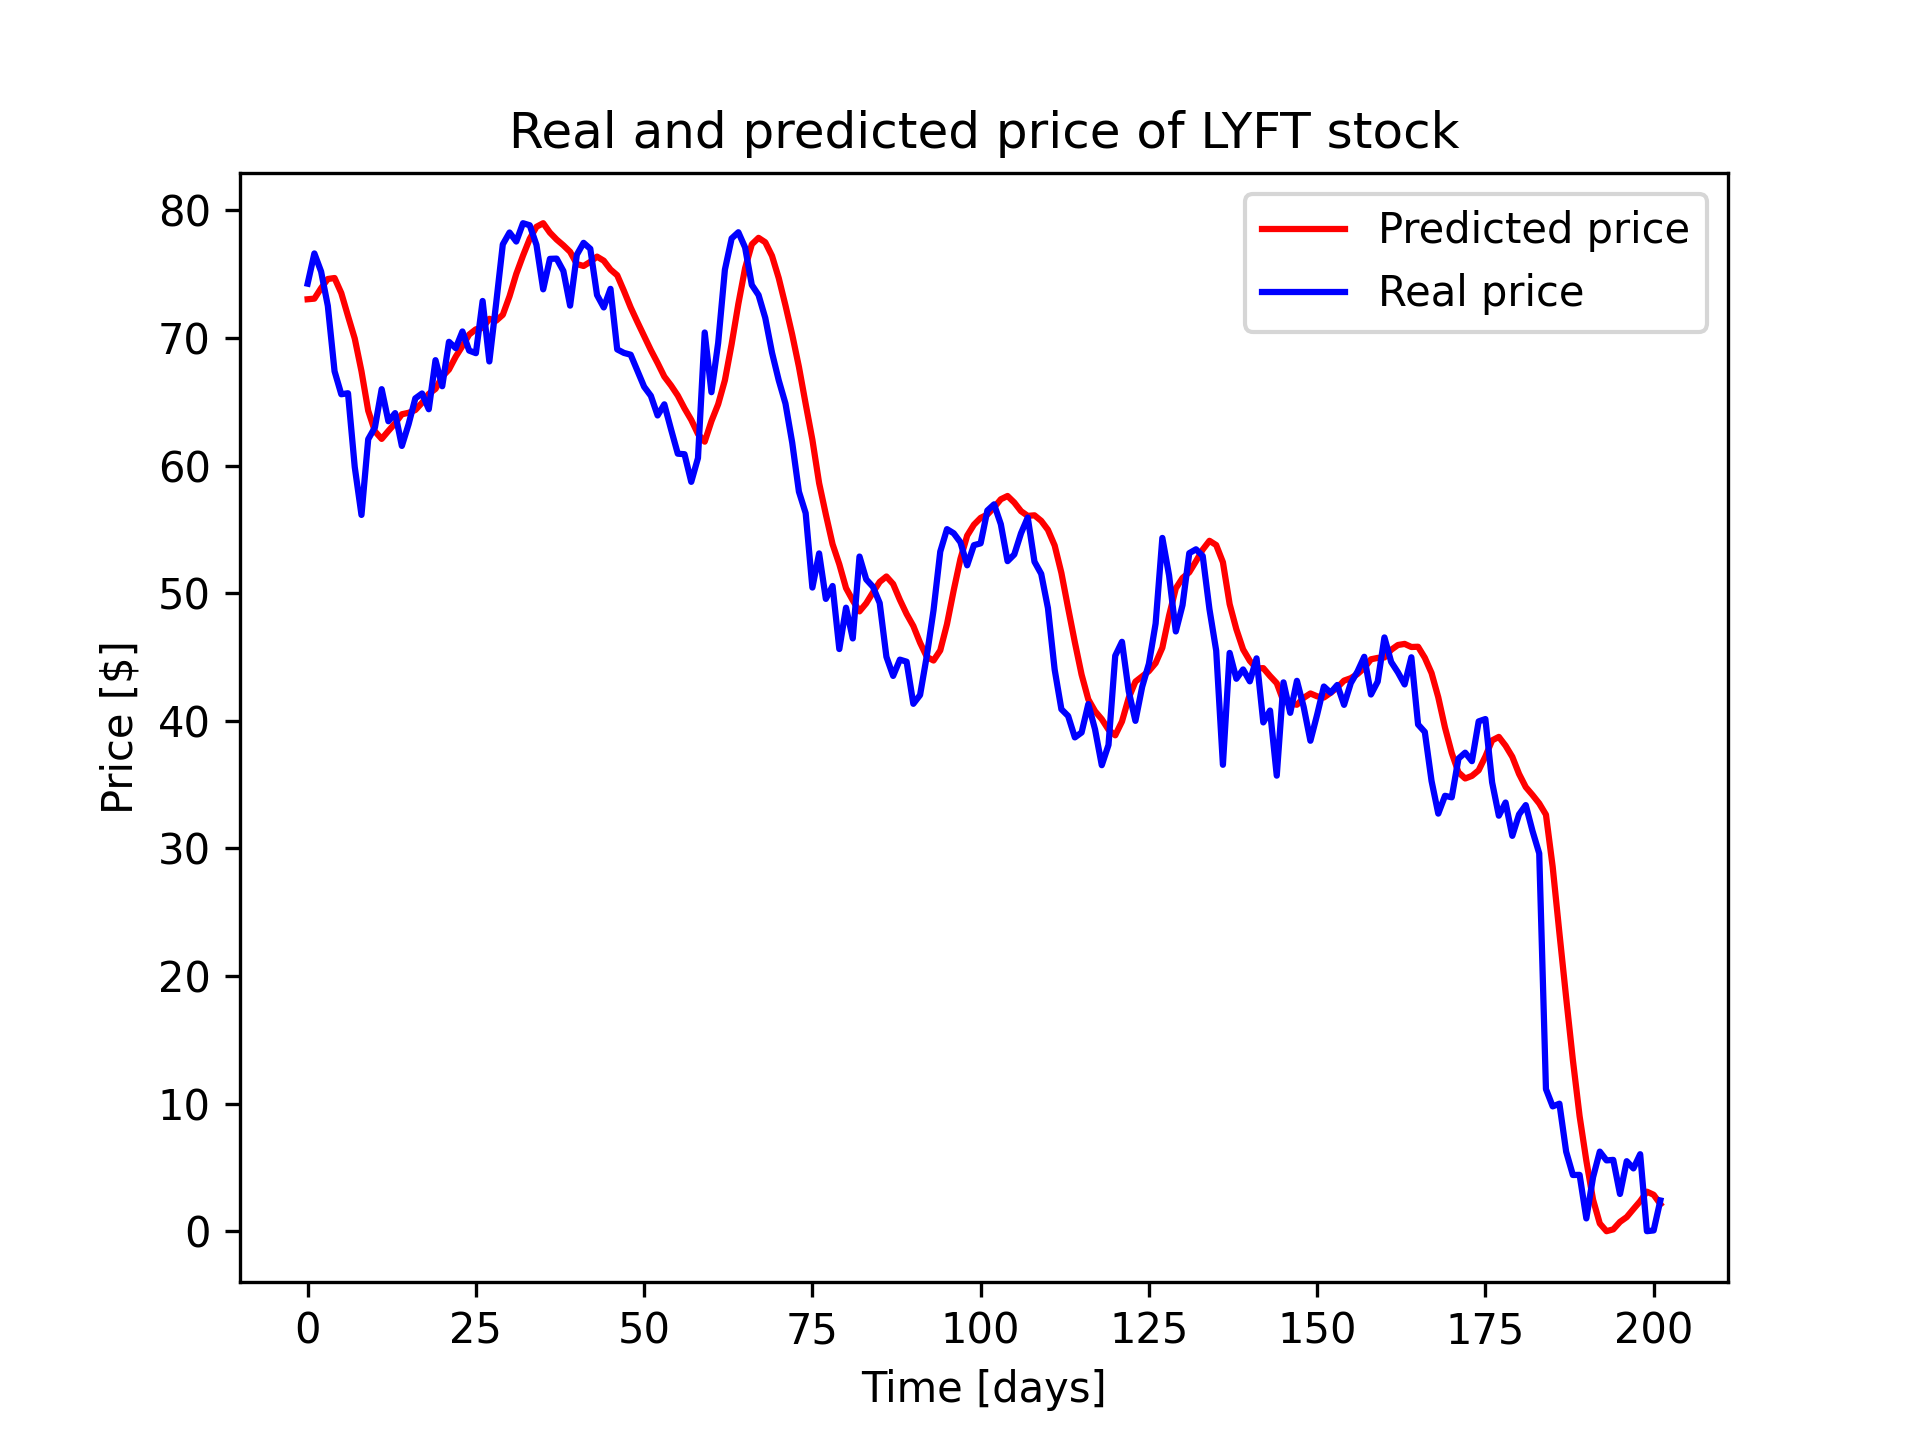
\includegraphics[width=0.5\textwidth]{./graf/model4/LYFT.png}
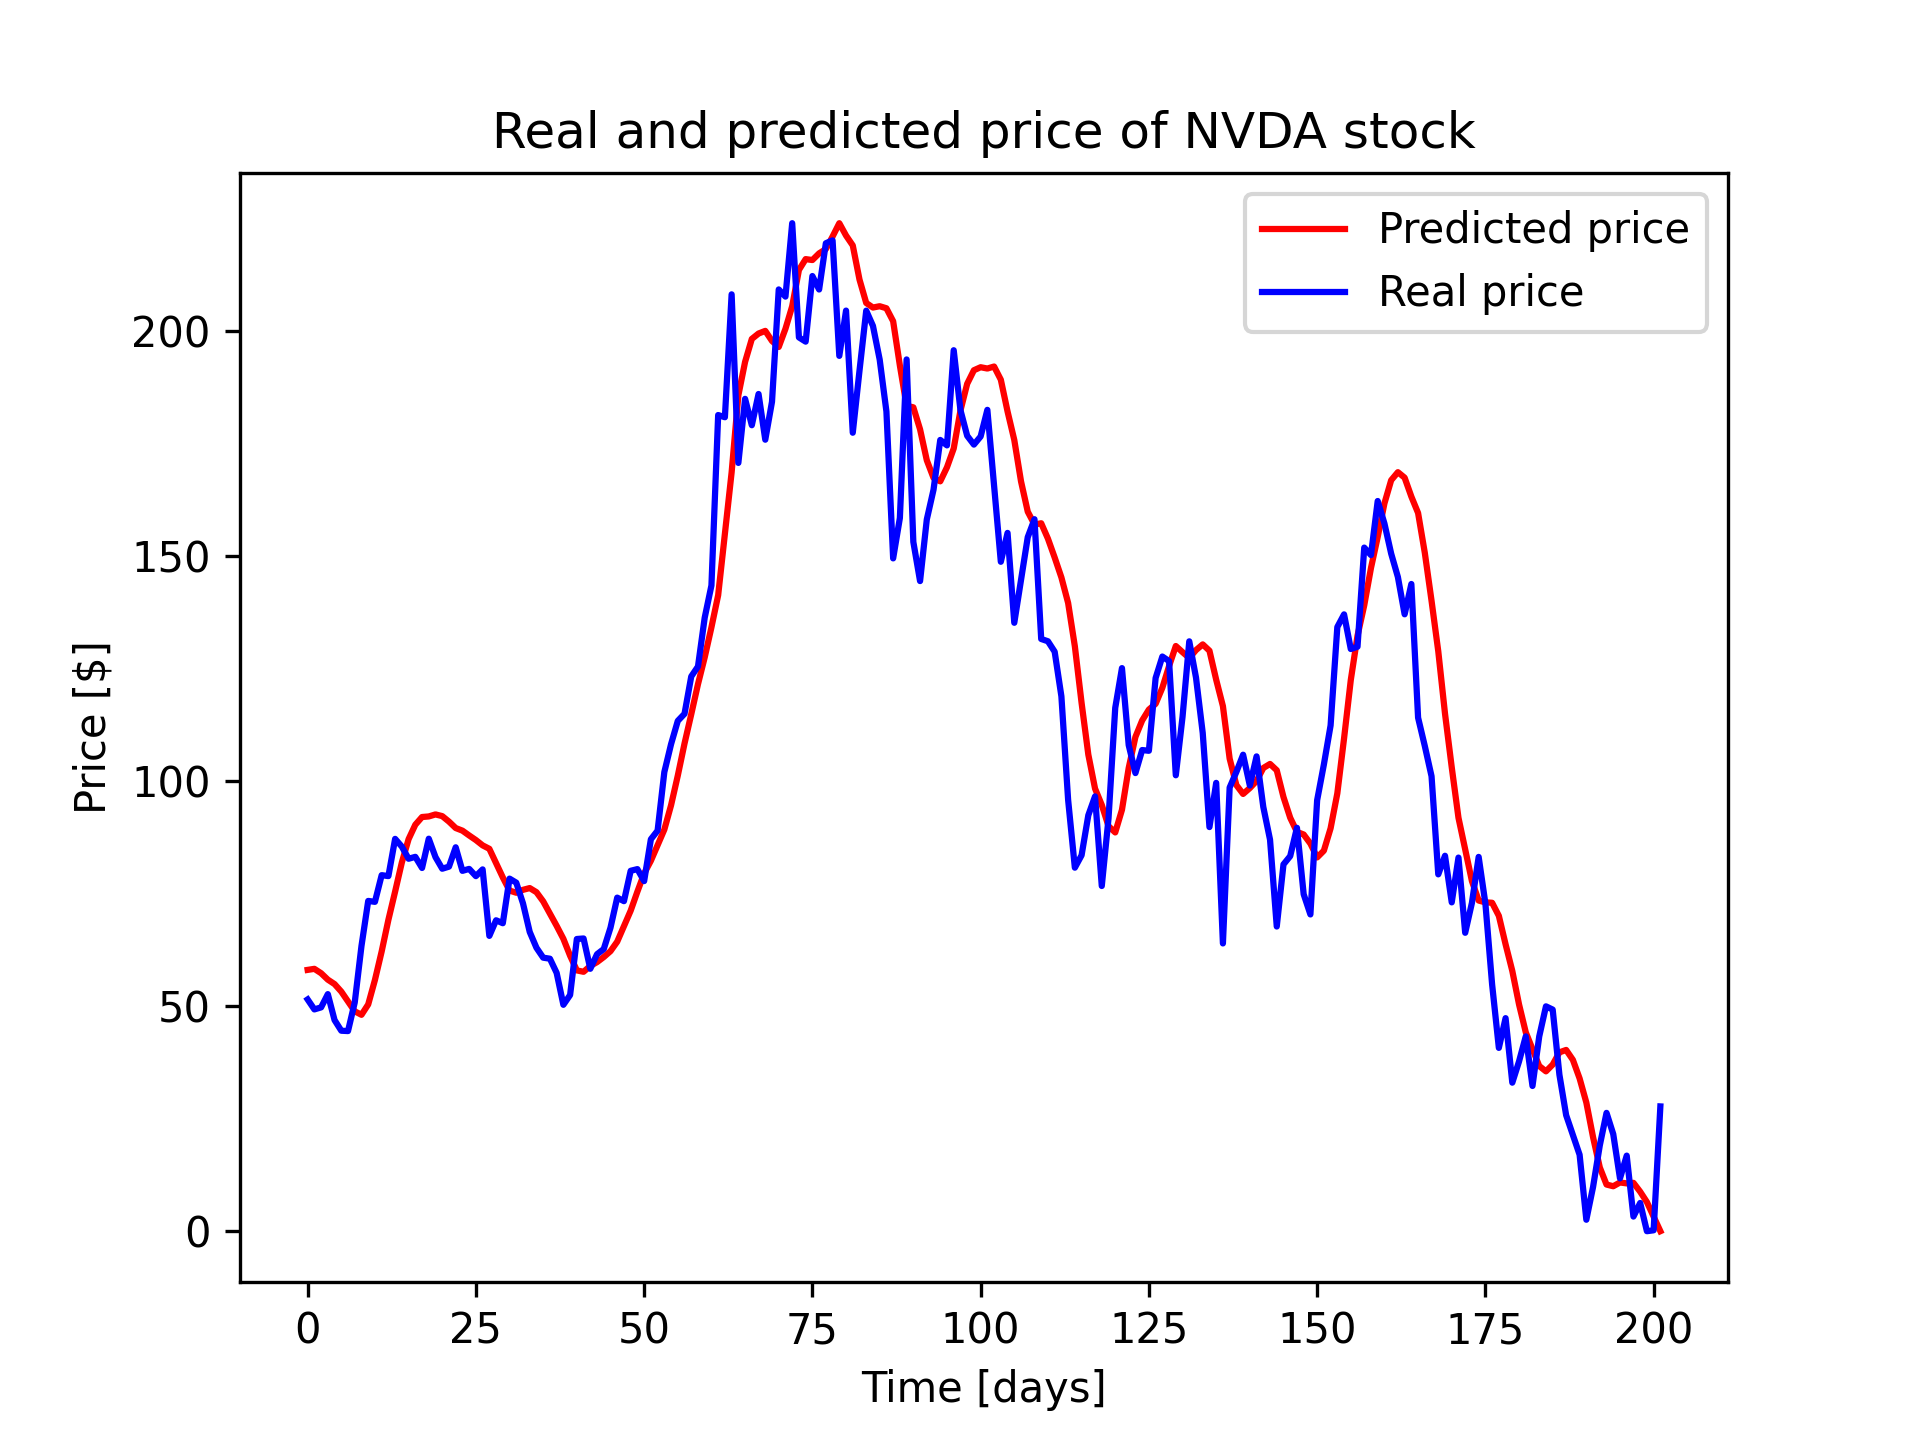
\includegraphics[width=0.5\textwidth]{./graf/model4/NVDA.png}
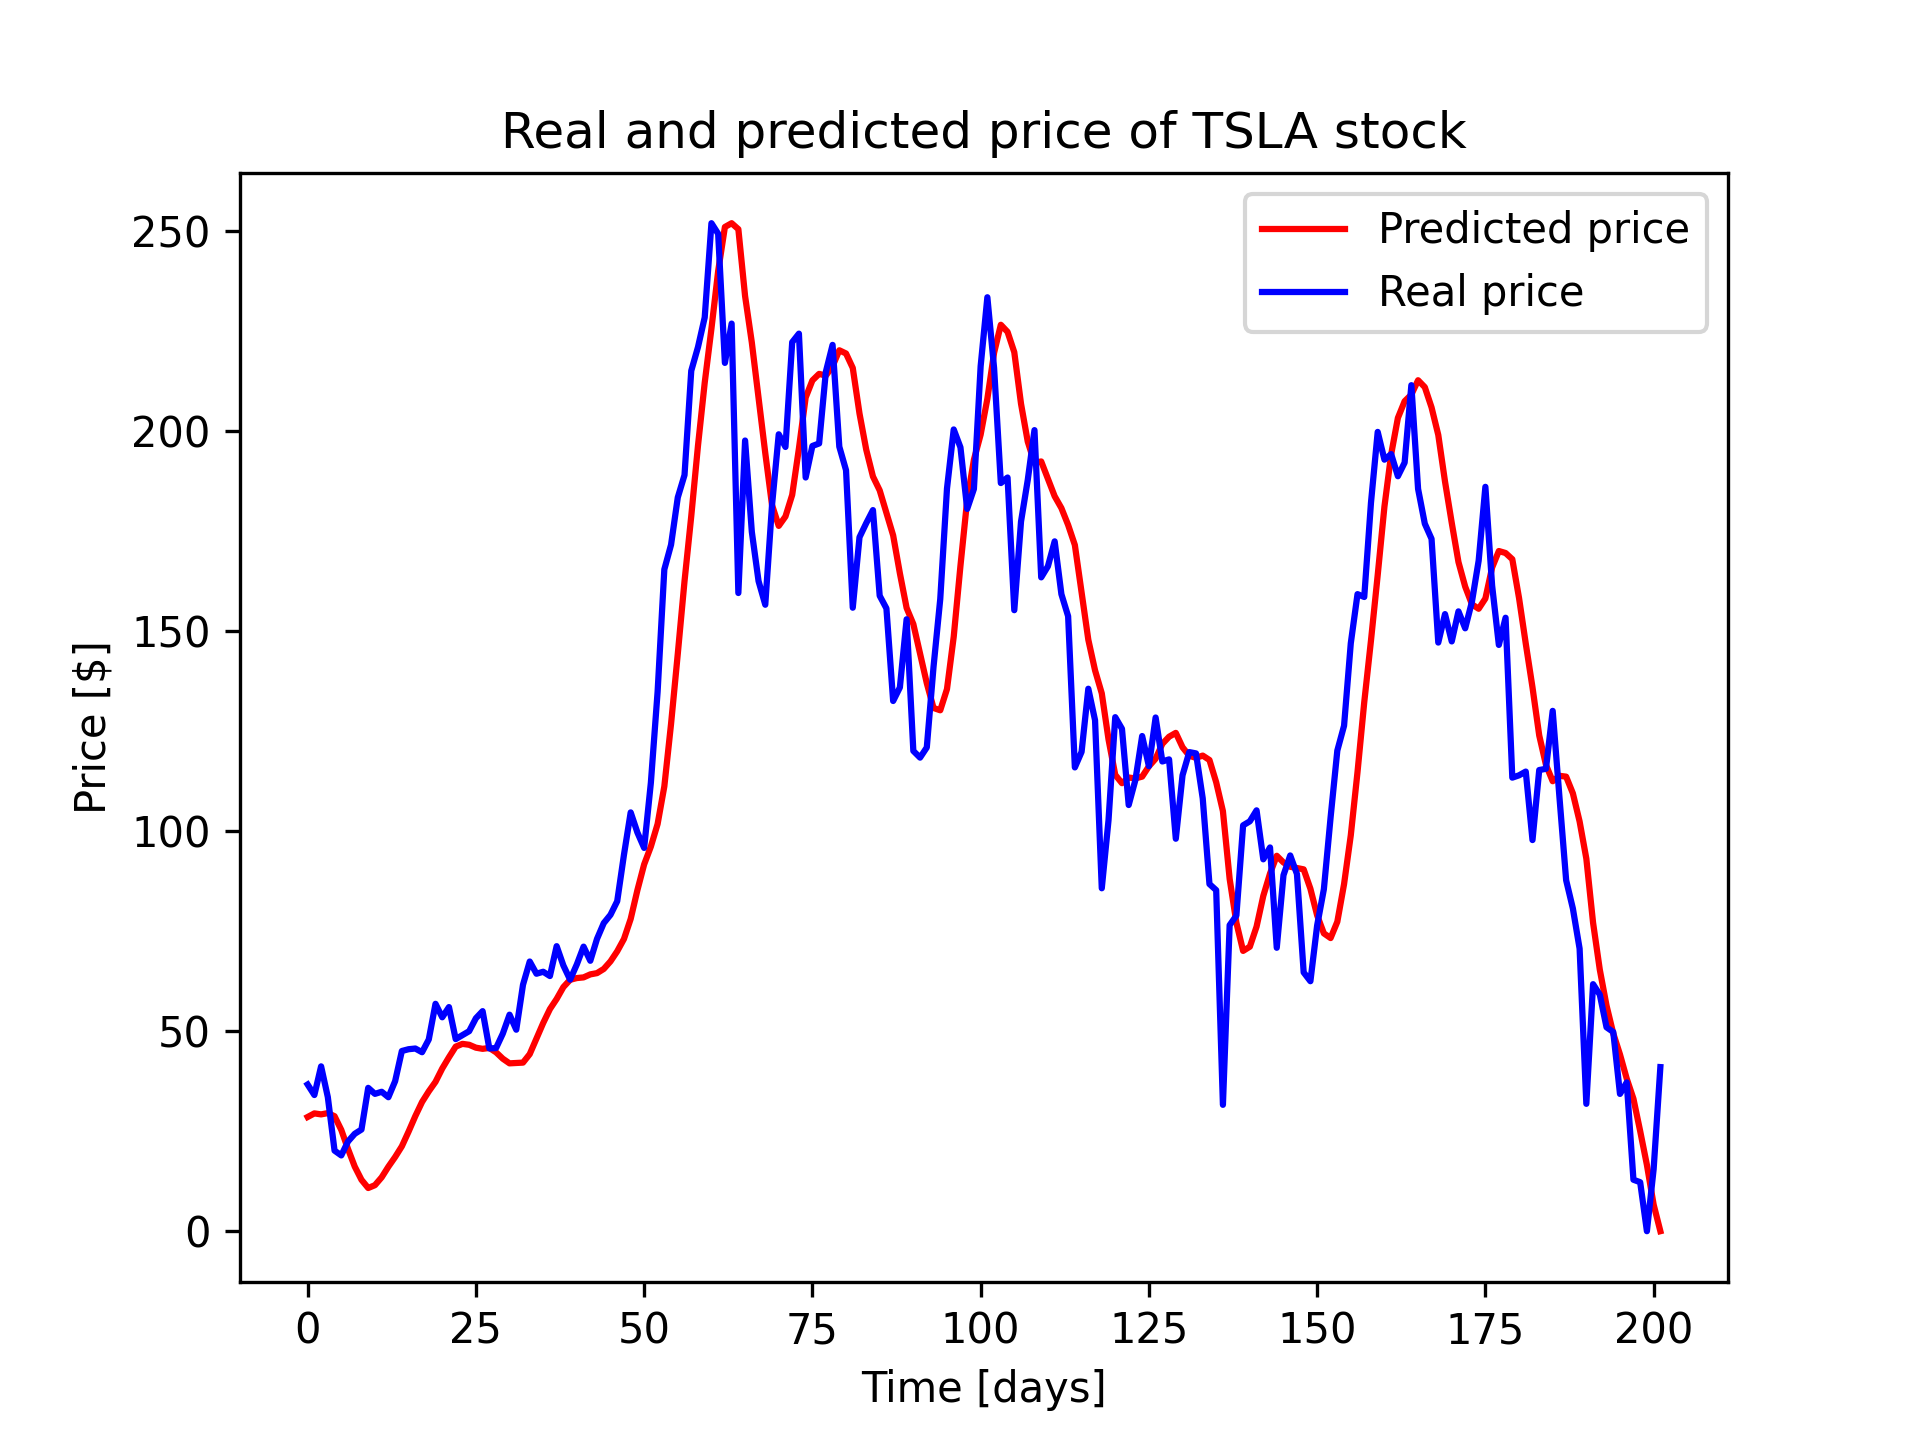
\includegraphics[width=0.5\textwidth]{./graf/model4/TSLA.png}
\caption{Real and predicted prices of the fourth model.}
\label{fig:label}
\end{figure} 

\clearpage
\subsection{Model 5}

Model5 - chunkSize: 50, time interval: 1 year, epochs: 10, trained on AAPL\par\bigskip
In this model, the lines showing the real price fluctuations and the price expected on the
market coincide in many areas. They show a systematic upward trend and a systematic decrease in
prices. However, it should be noted that sudden deflections were not depicted here by the course of
the red line. The red line does not reach its apogee if the deflection amplitude is large and sudden.

\begin{figure}
% \centering
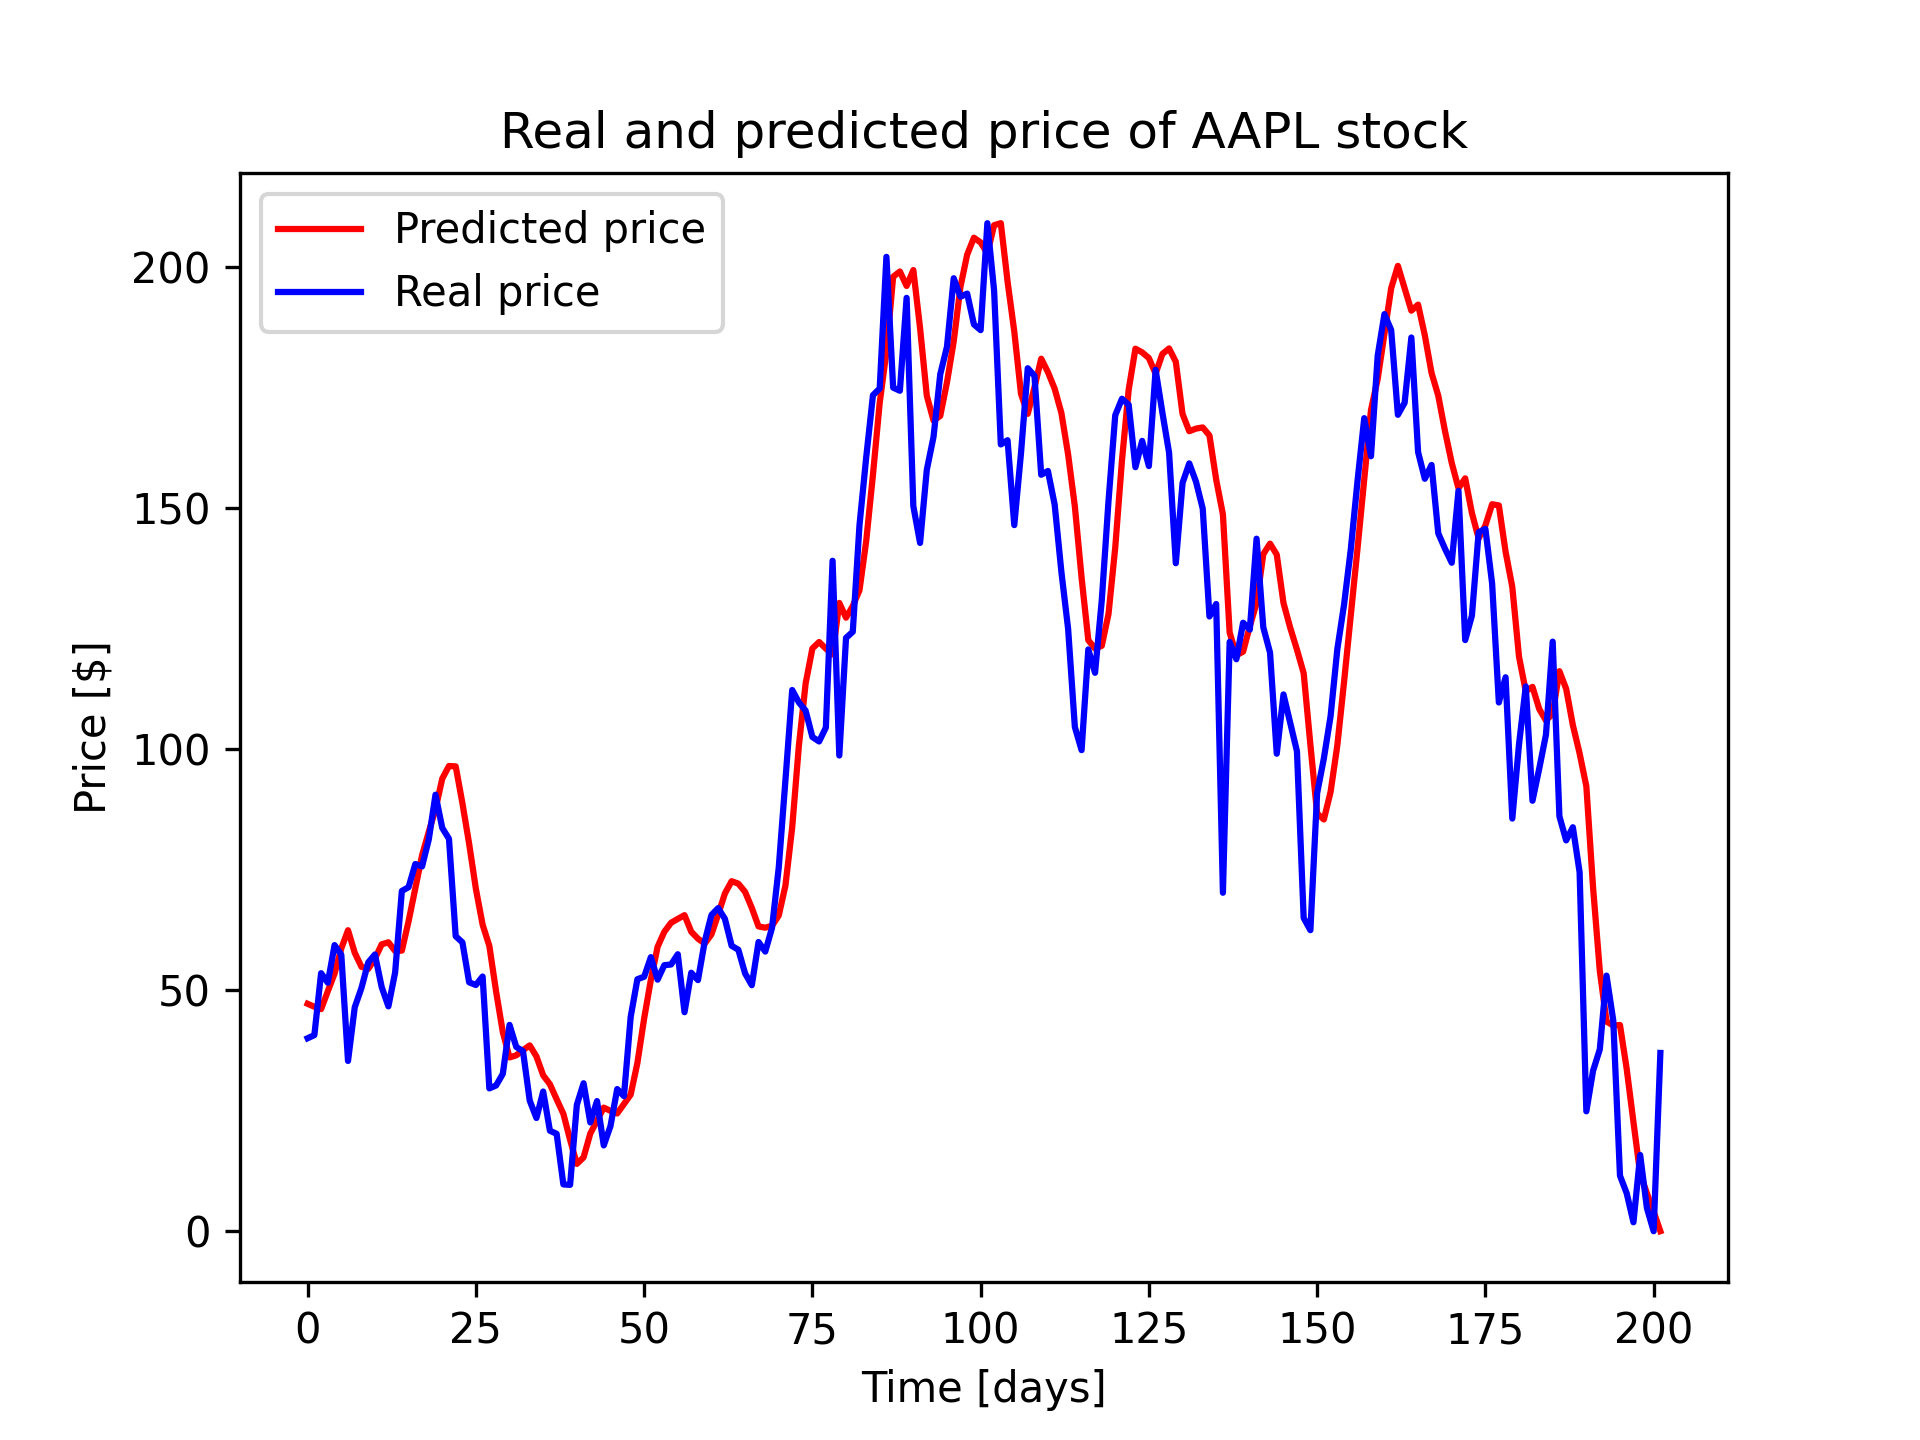
\includegraphics[width=0.5\textwidth]{./graf/model5/AAPL.png}
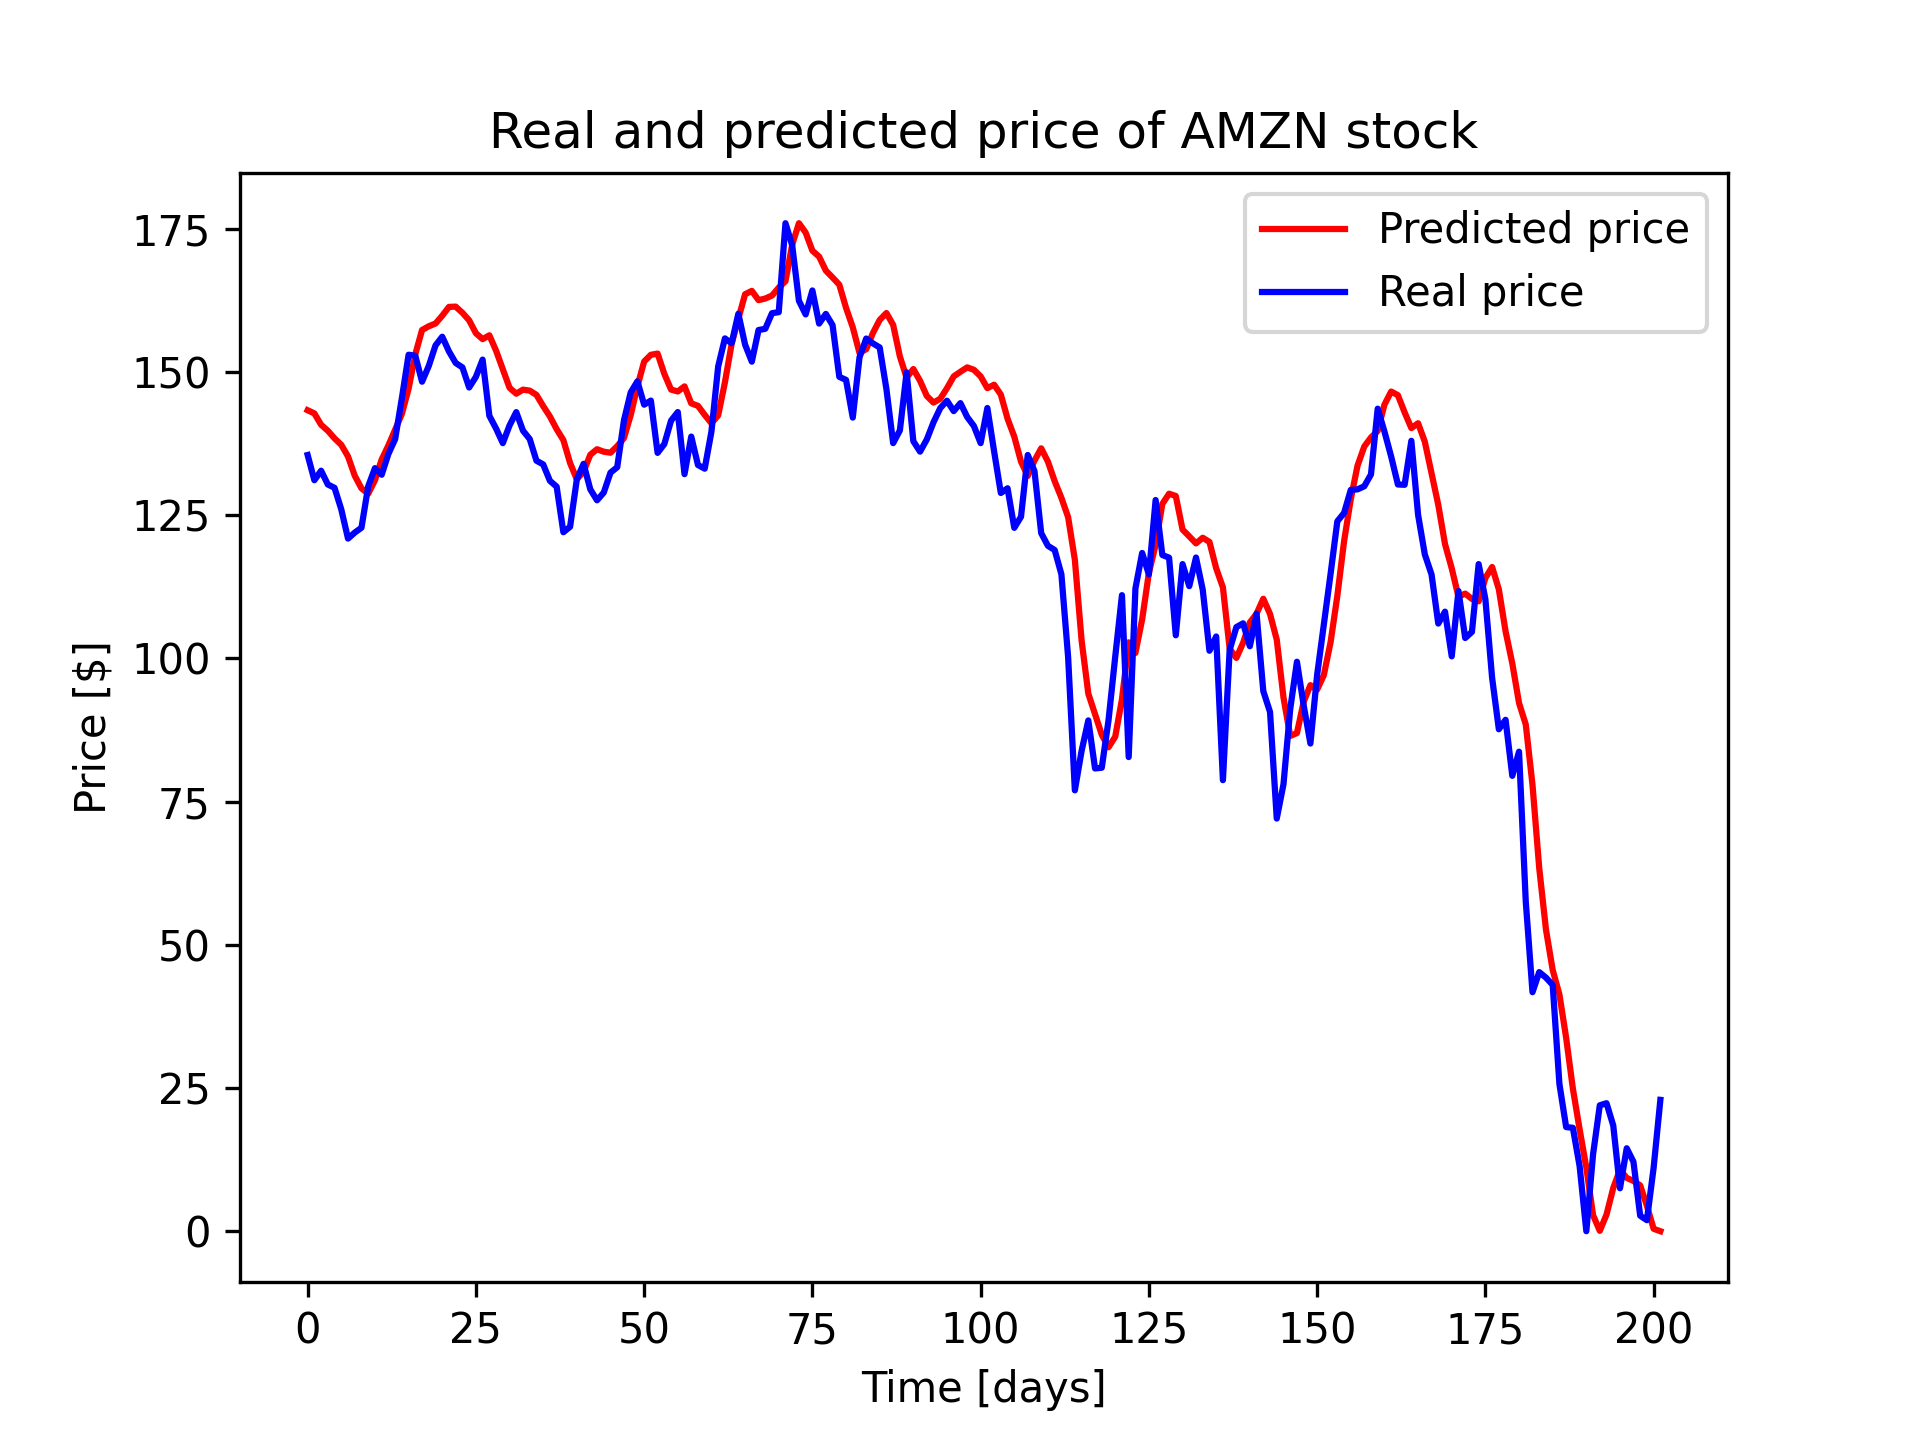
\includegraphics[width=0.5\textwidth]{./graf/model5/AMZN.png}
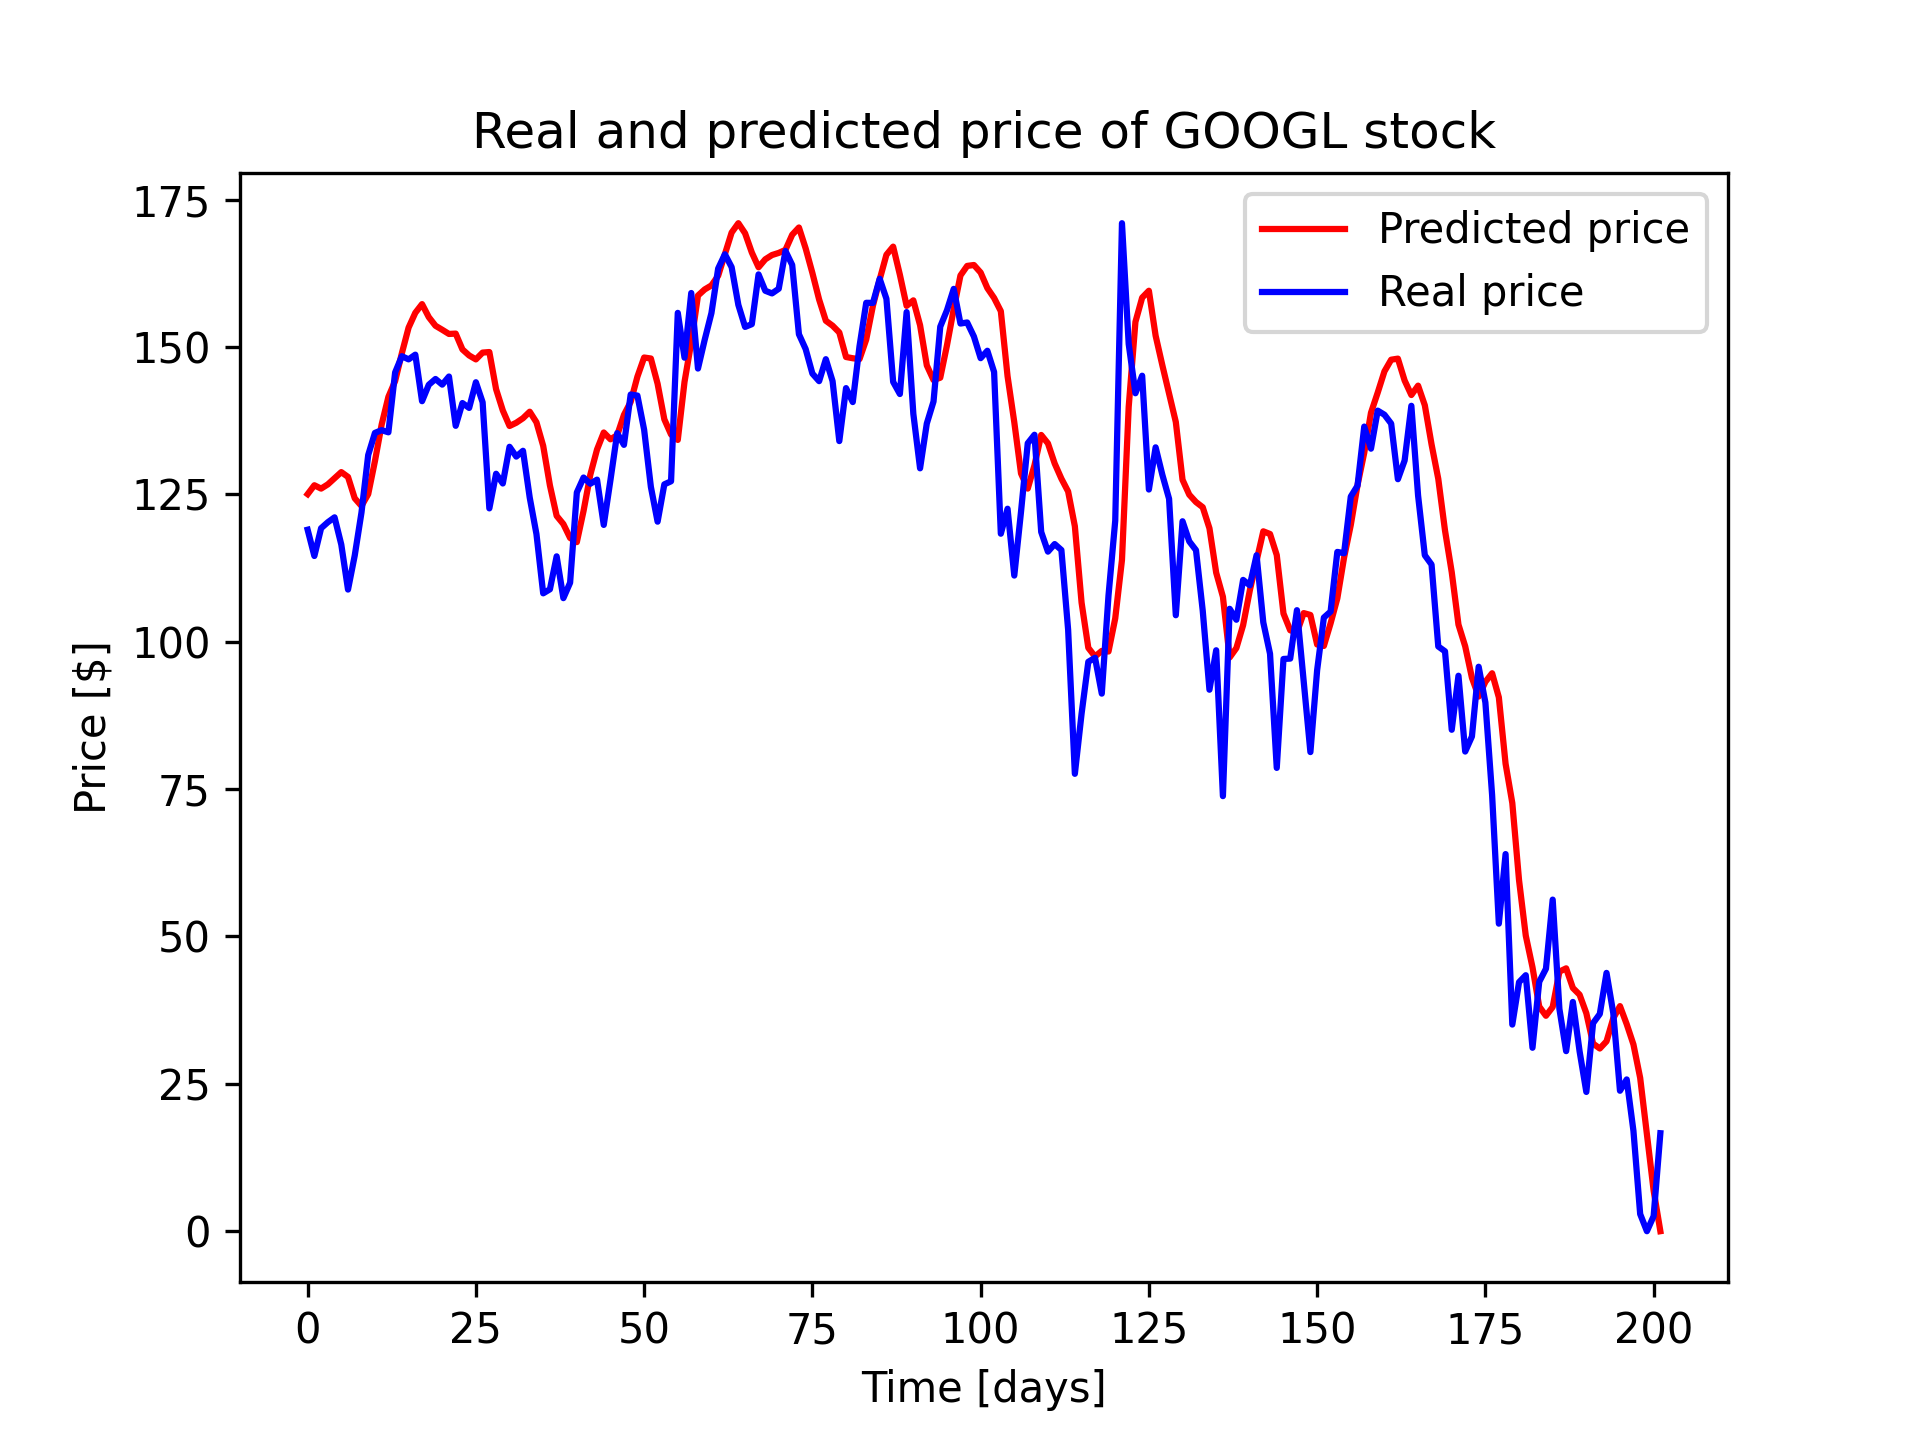
\includegraphics[width=0.5\textwidth]{./graf/model5/GOOGL.png}
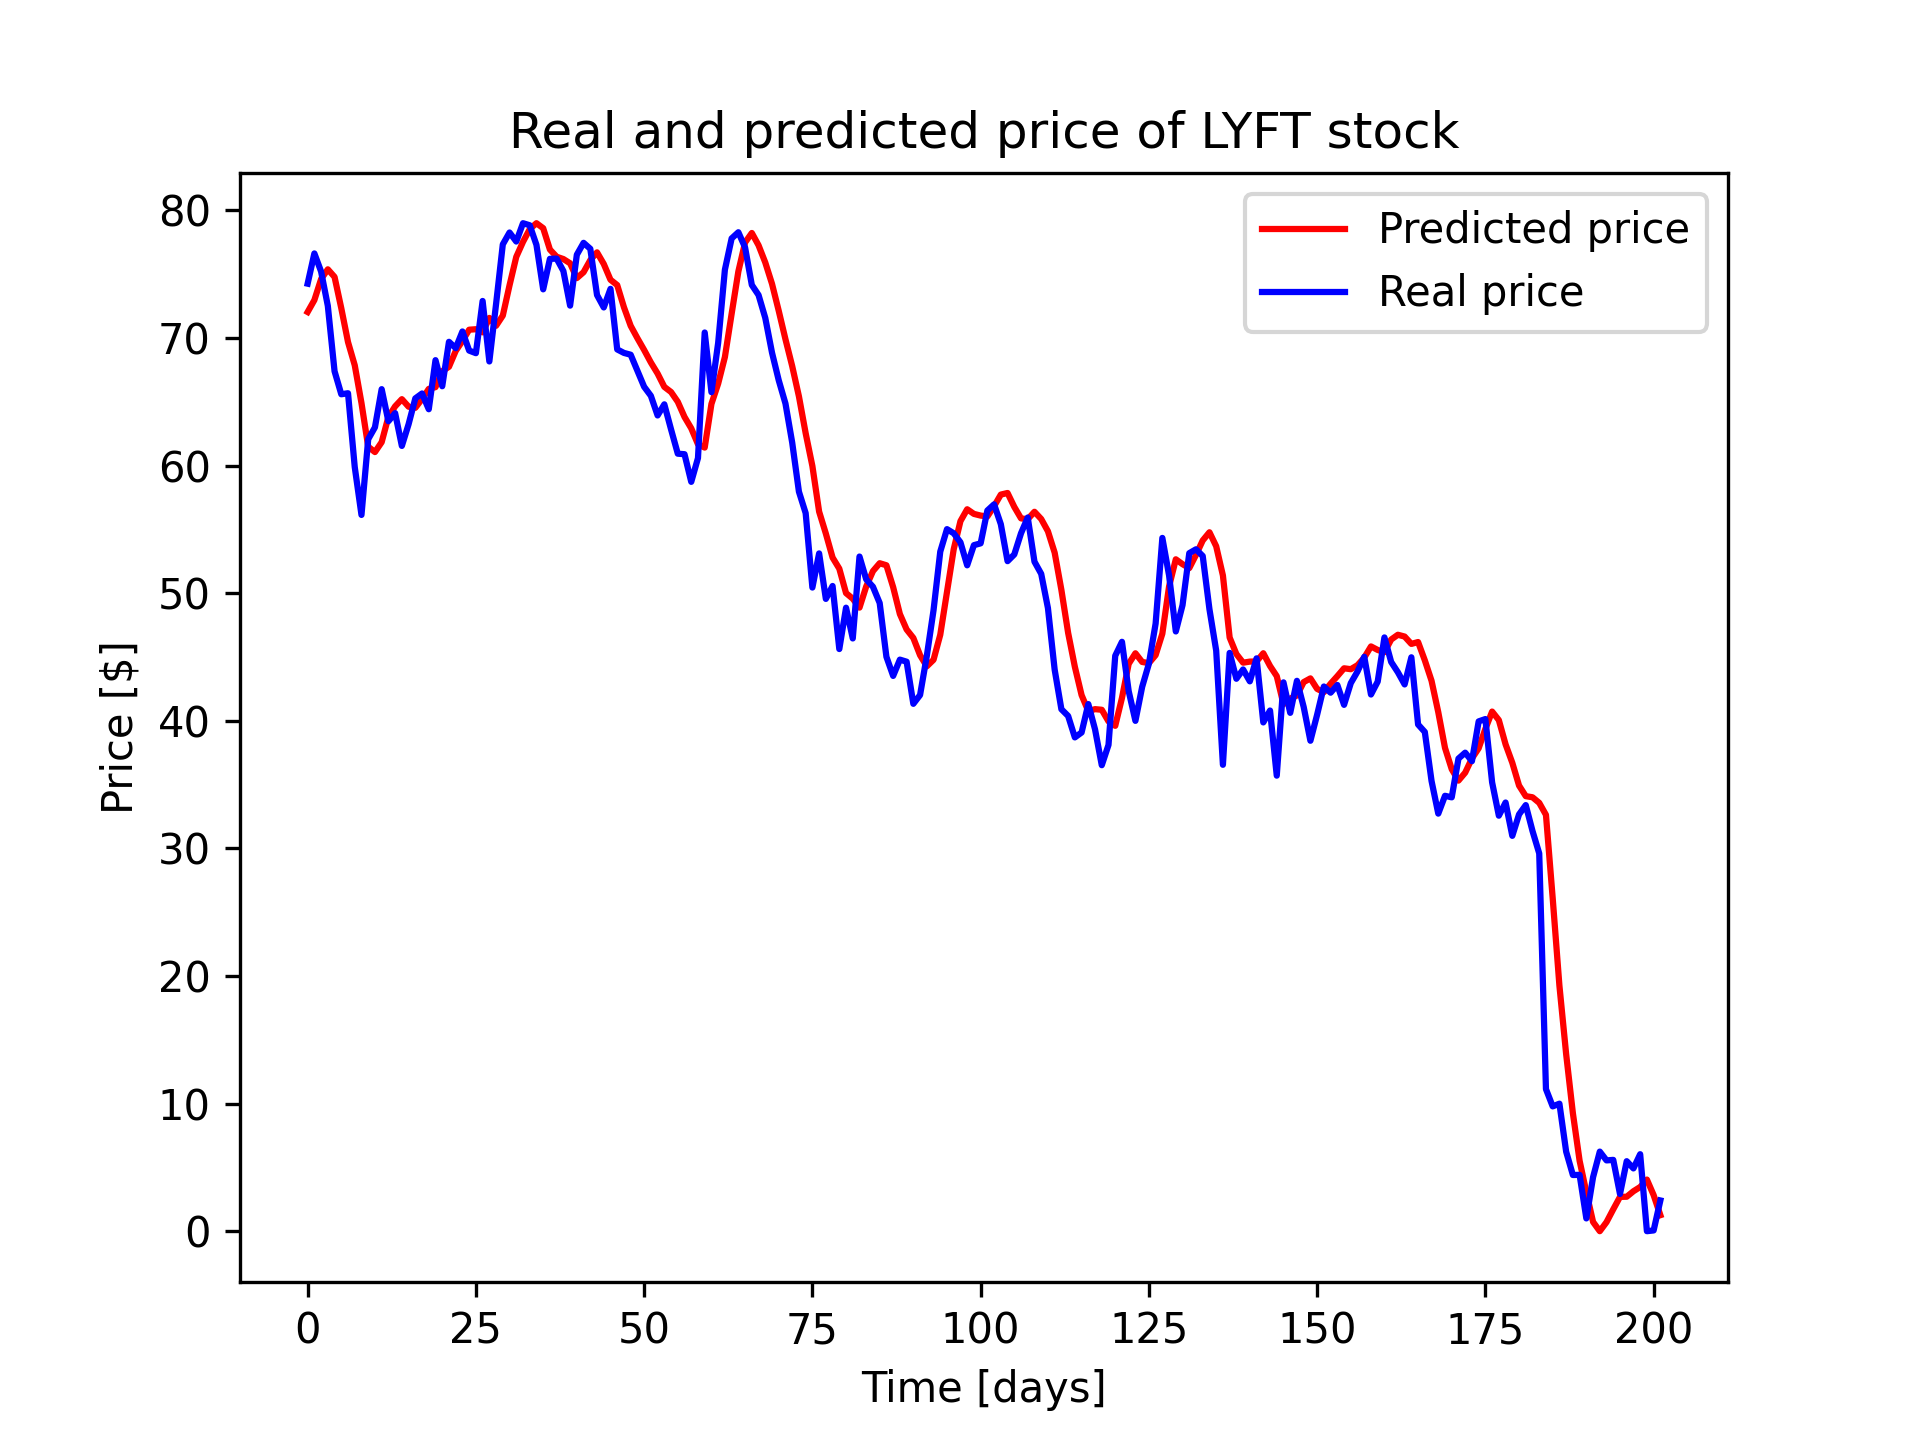
\includegraphics[width=0.5\textwidth]{./graf/model5/LYFT.png}
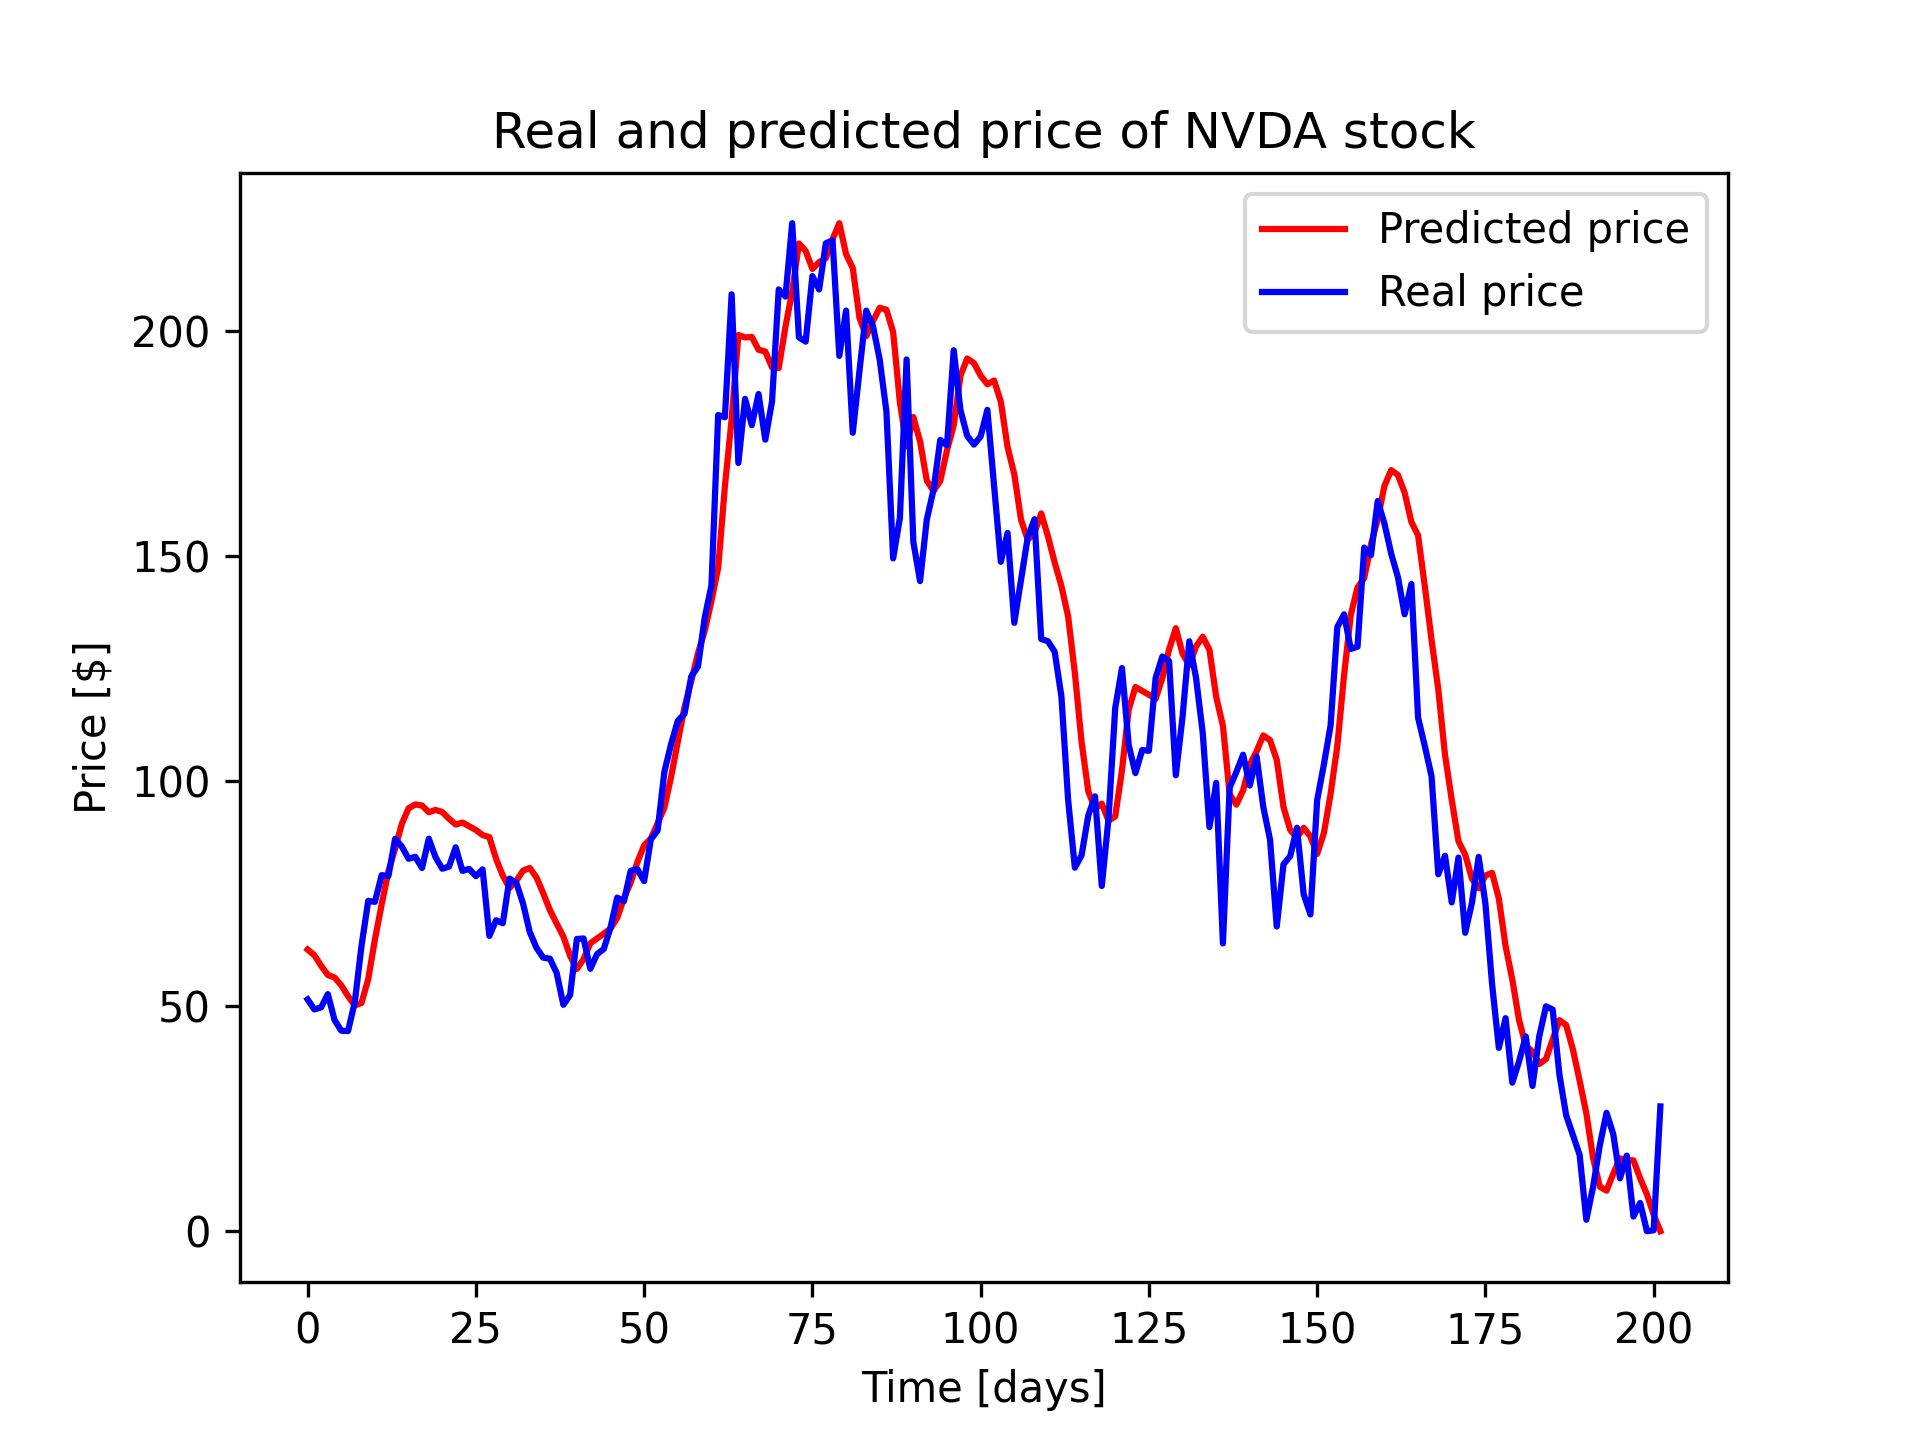
\includegraphics[width=0.5\textwidth]{./graf/model5/NVDA.png}
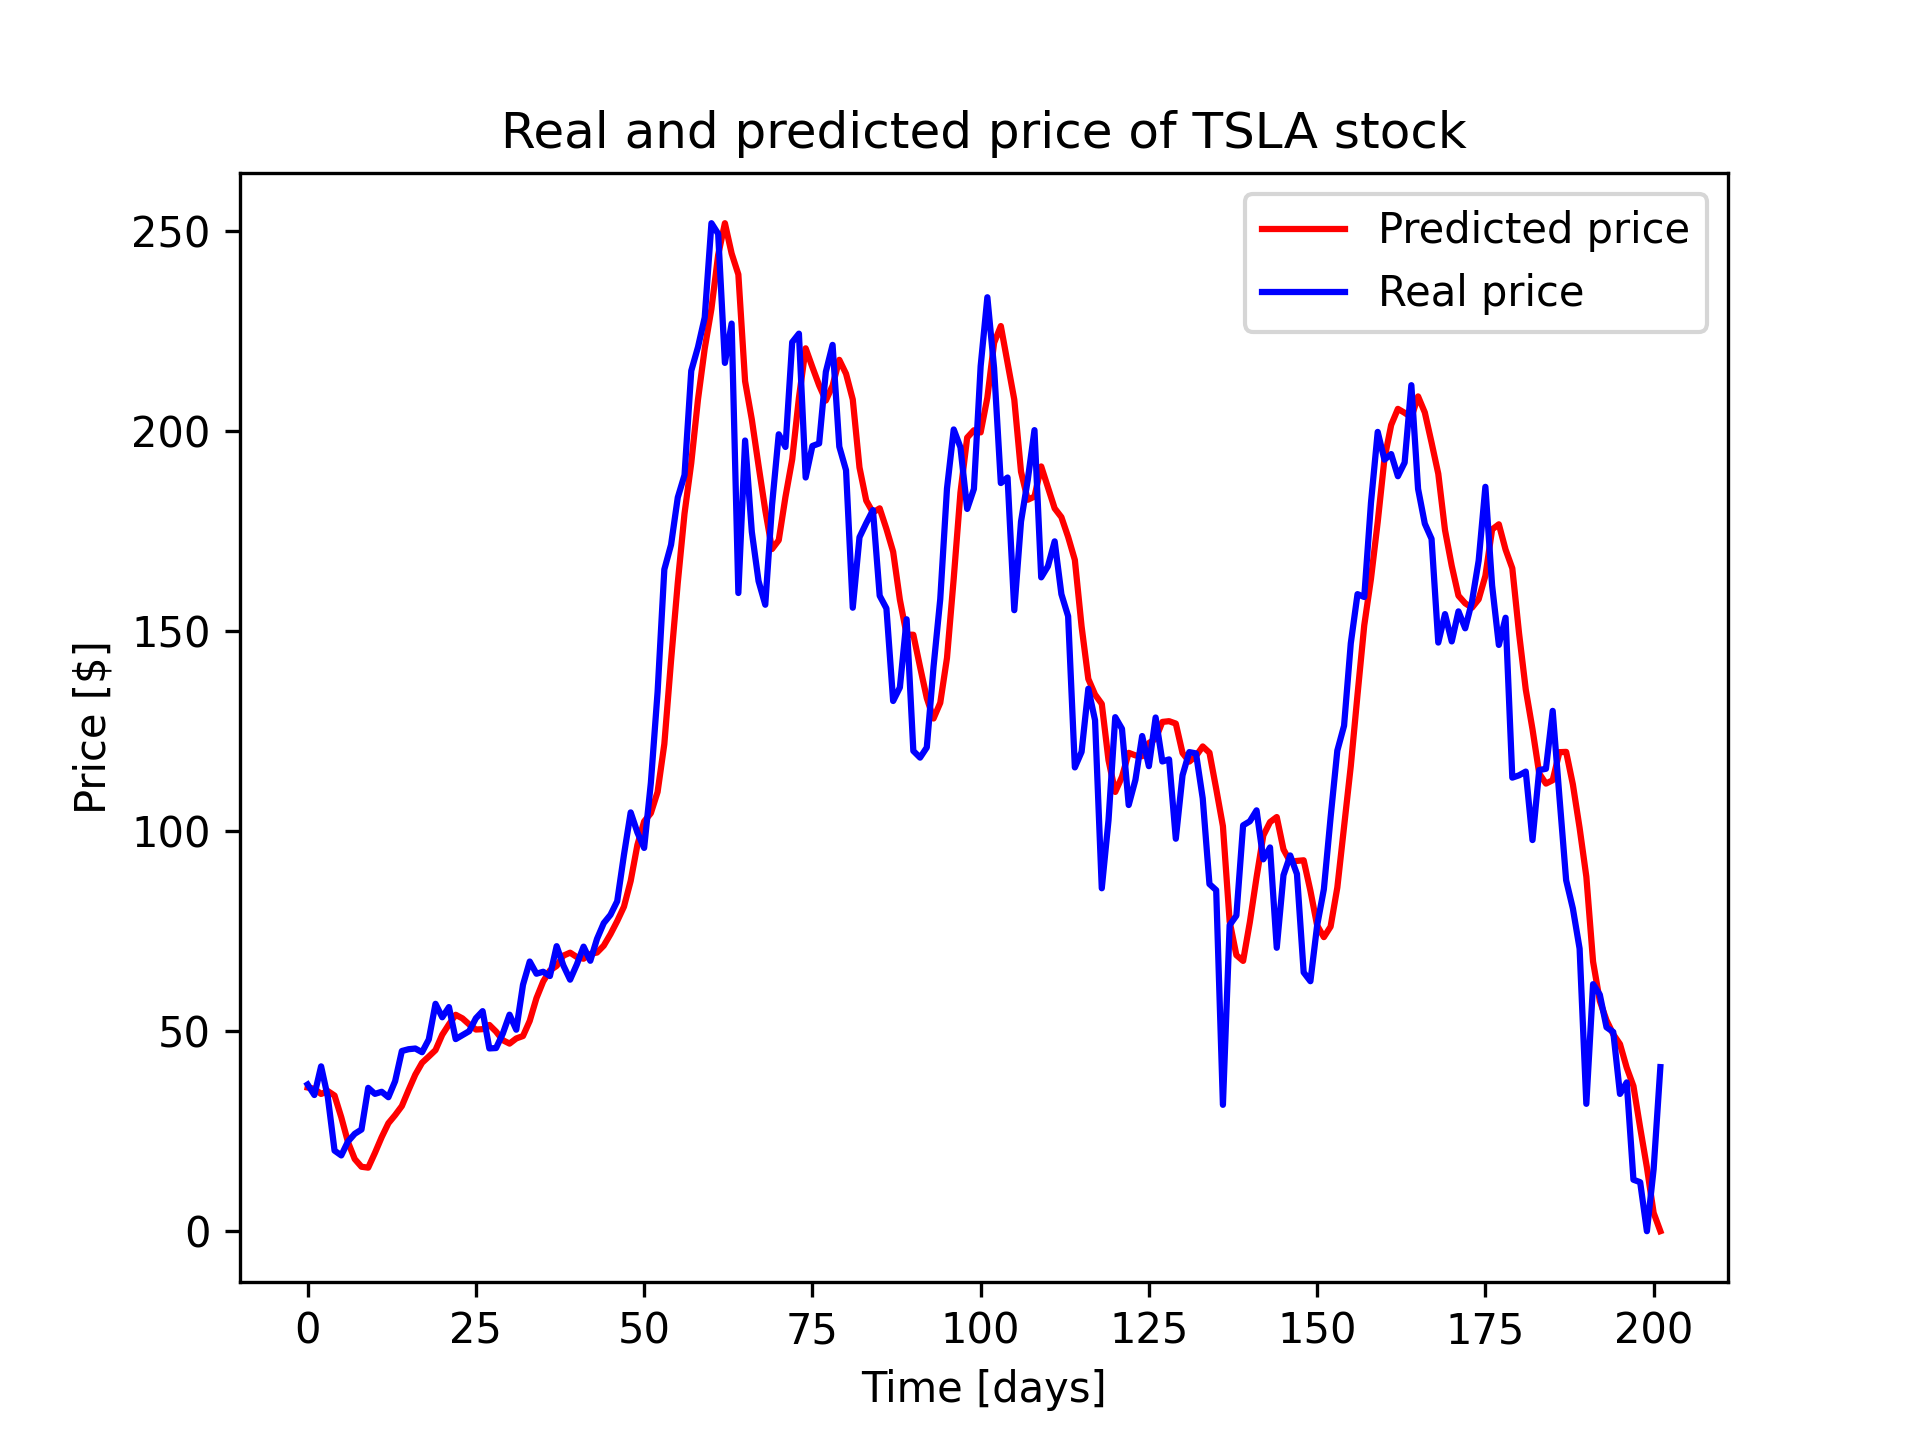
\includegraphics[width=0.5\textwidth]{./graf/model5/TSLA.png}
\caption{Real and predicted prices of the fifth model.}
\label{fig:label}
\end{figure} 

\clearpage
\subsection{Model 6}

Model6 - chunkSize: 50, time interval: 1 year, epochs: 15, trained on AAPL\par\bigskip
Observing the deflections of the line in model 6, it can be observed that the course of both lines does
not always coincide over their entire course. Analyzing the path of the red line, it can be seen that it
runs above the blue line. Given the horizontal shift, it runs to the right of the blue line. When
considering situations where prices go up or down systematically, both lines coincide, which is worth
noting. On the other hand, sudden price drops shown in the blue line are not reflected in the course
of the red line. This situation is most marked in the graph for AAPL.png., and GOOGL.png.

\begin{figure}
% \centering
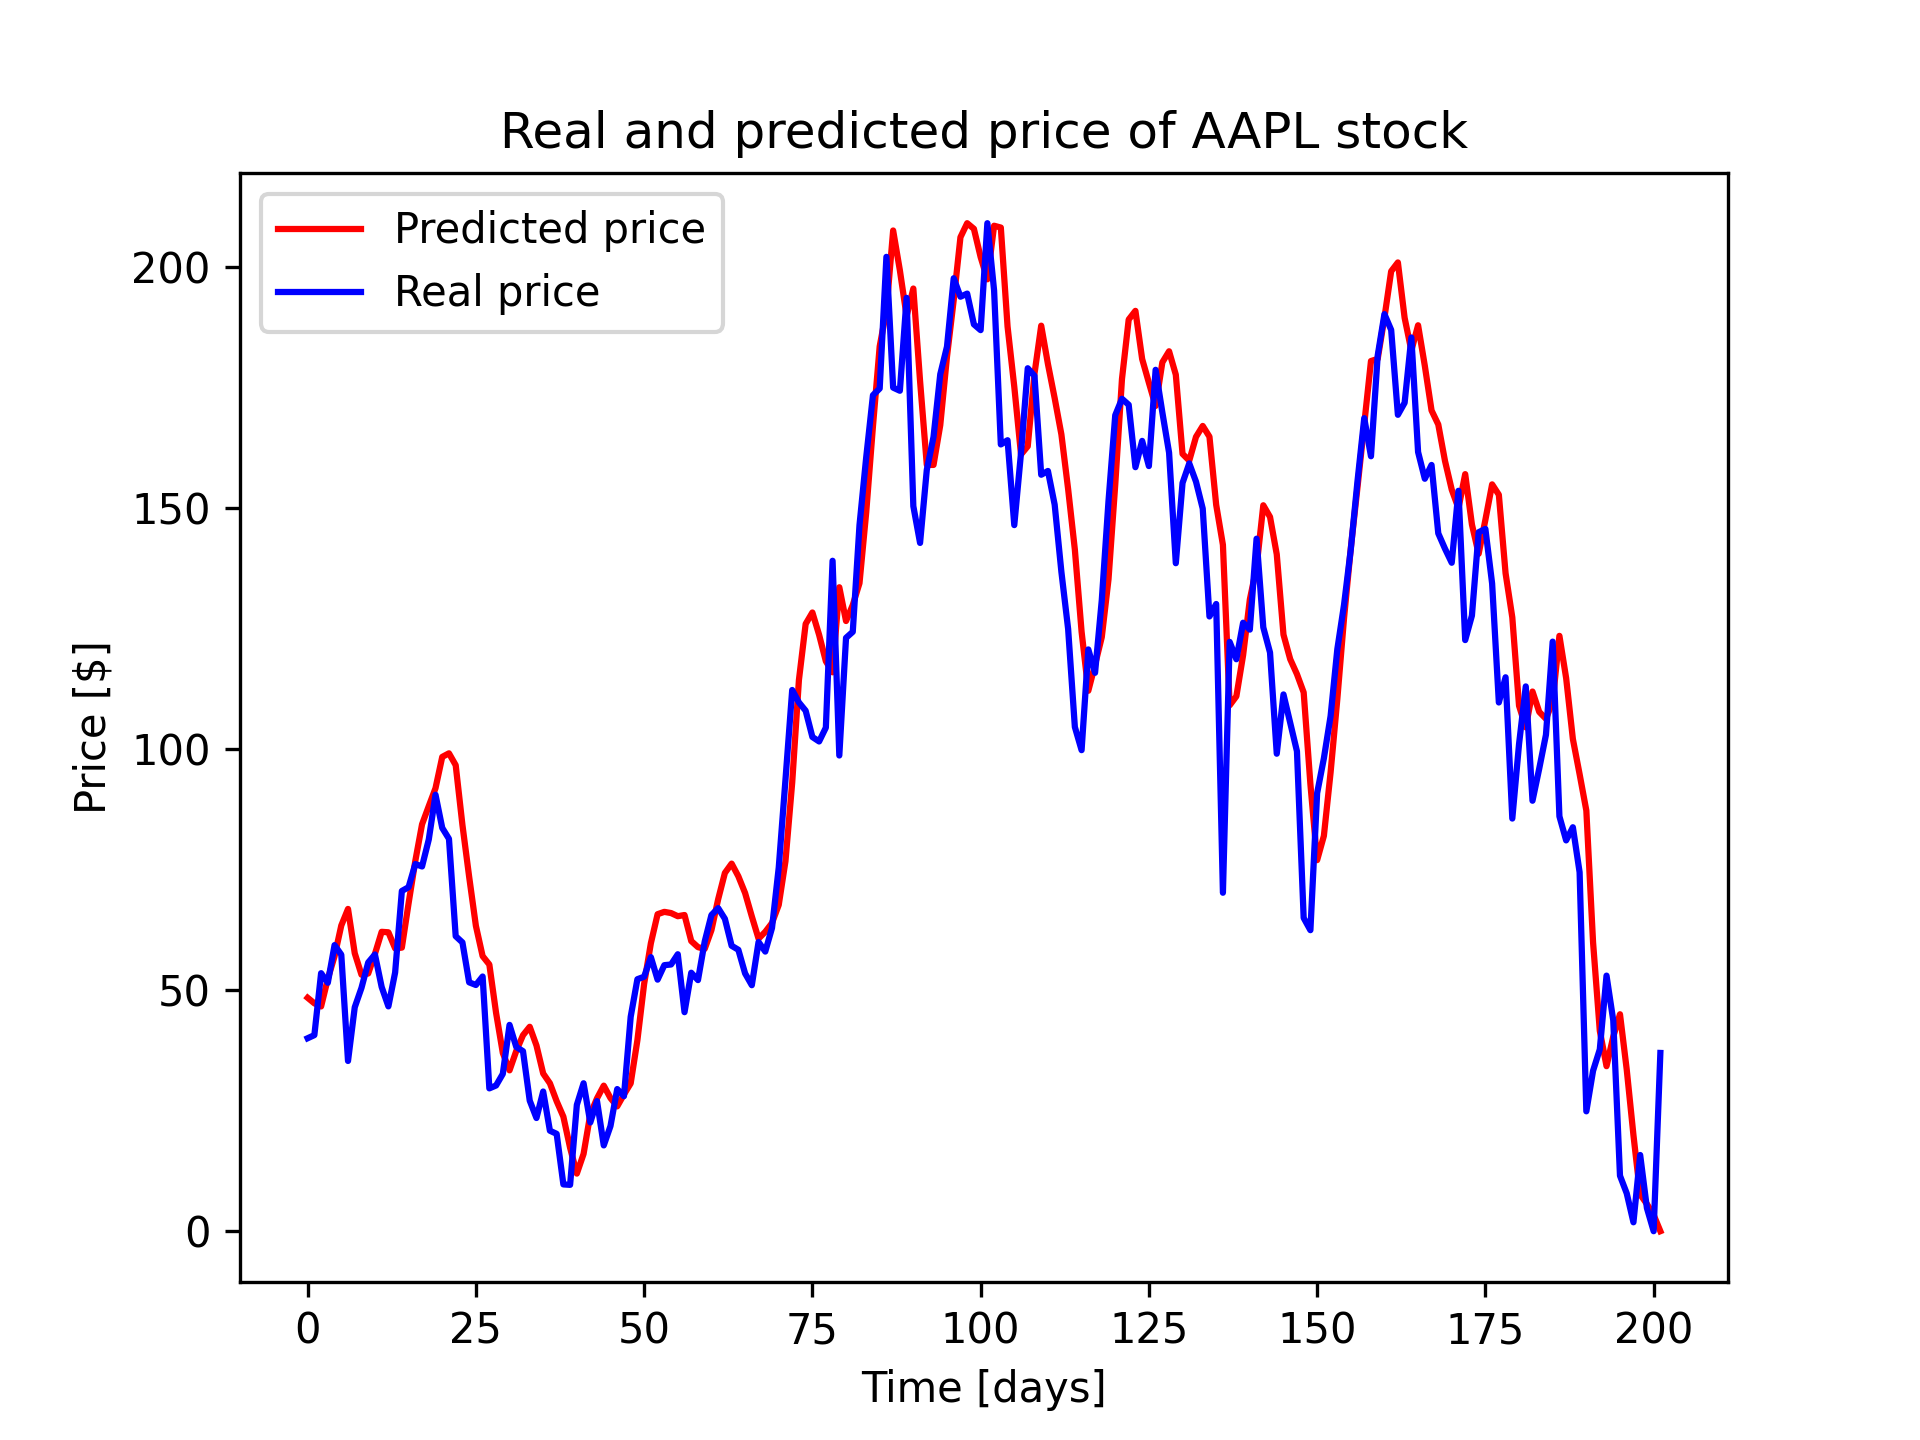
\includegraphics[width=0.5\textwidth]{./graf/model6/AAPL.png}
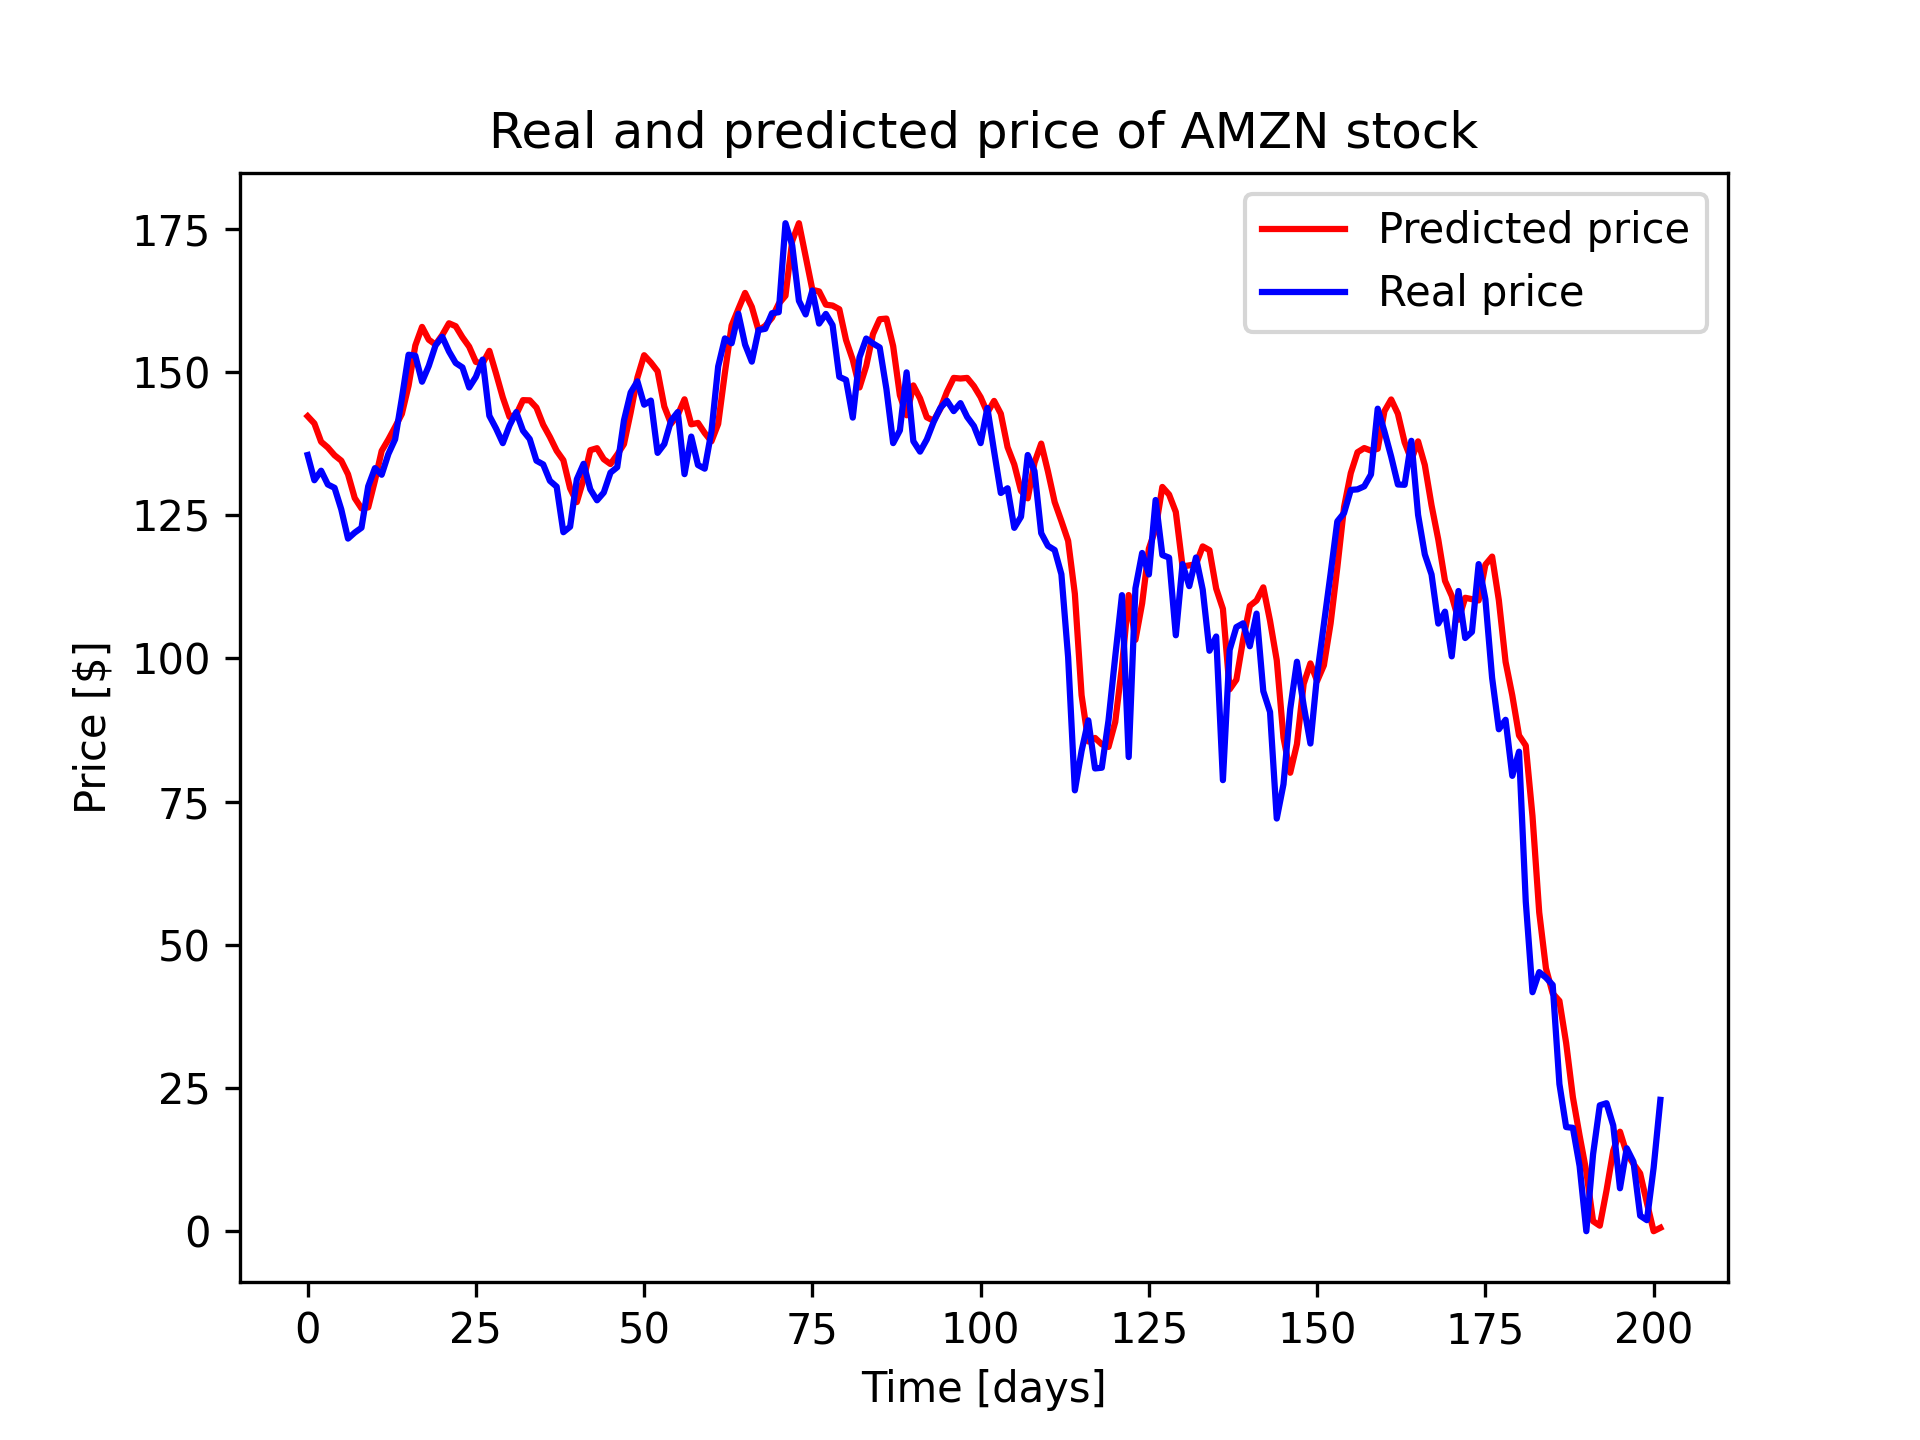
\includegraphics[width=0.5\textwidth]{./graf/model6/AMZN.png}
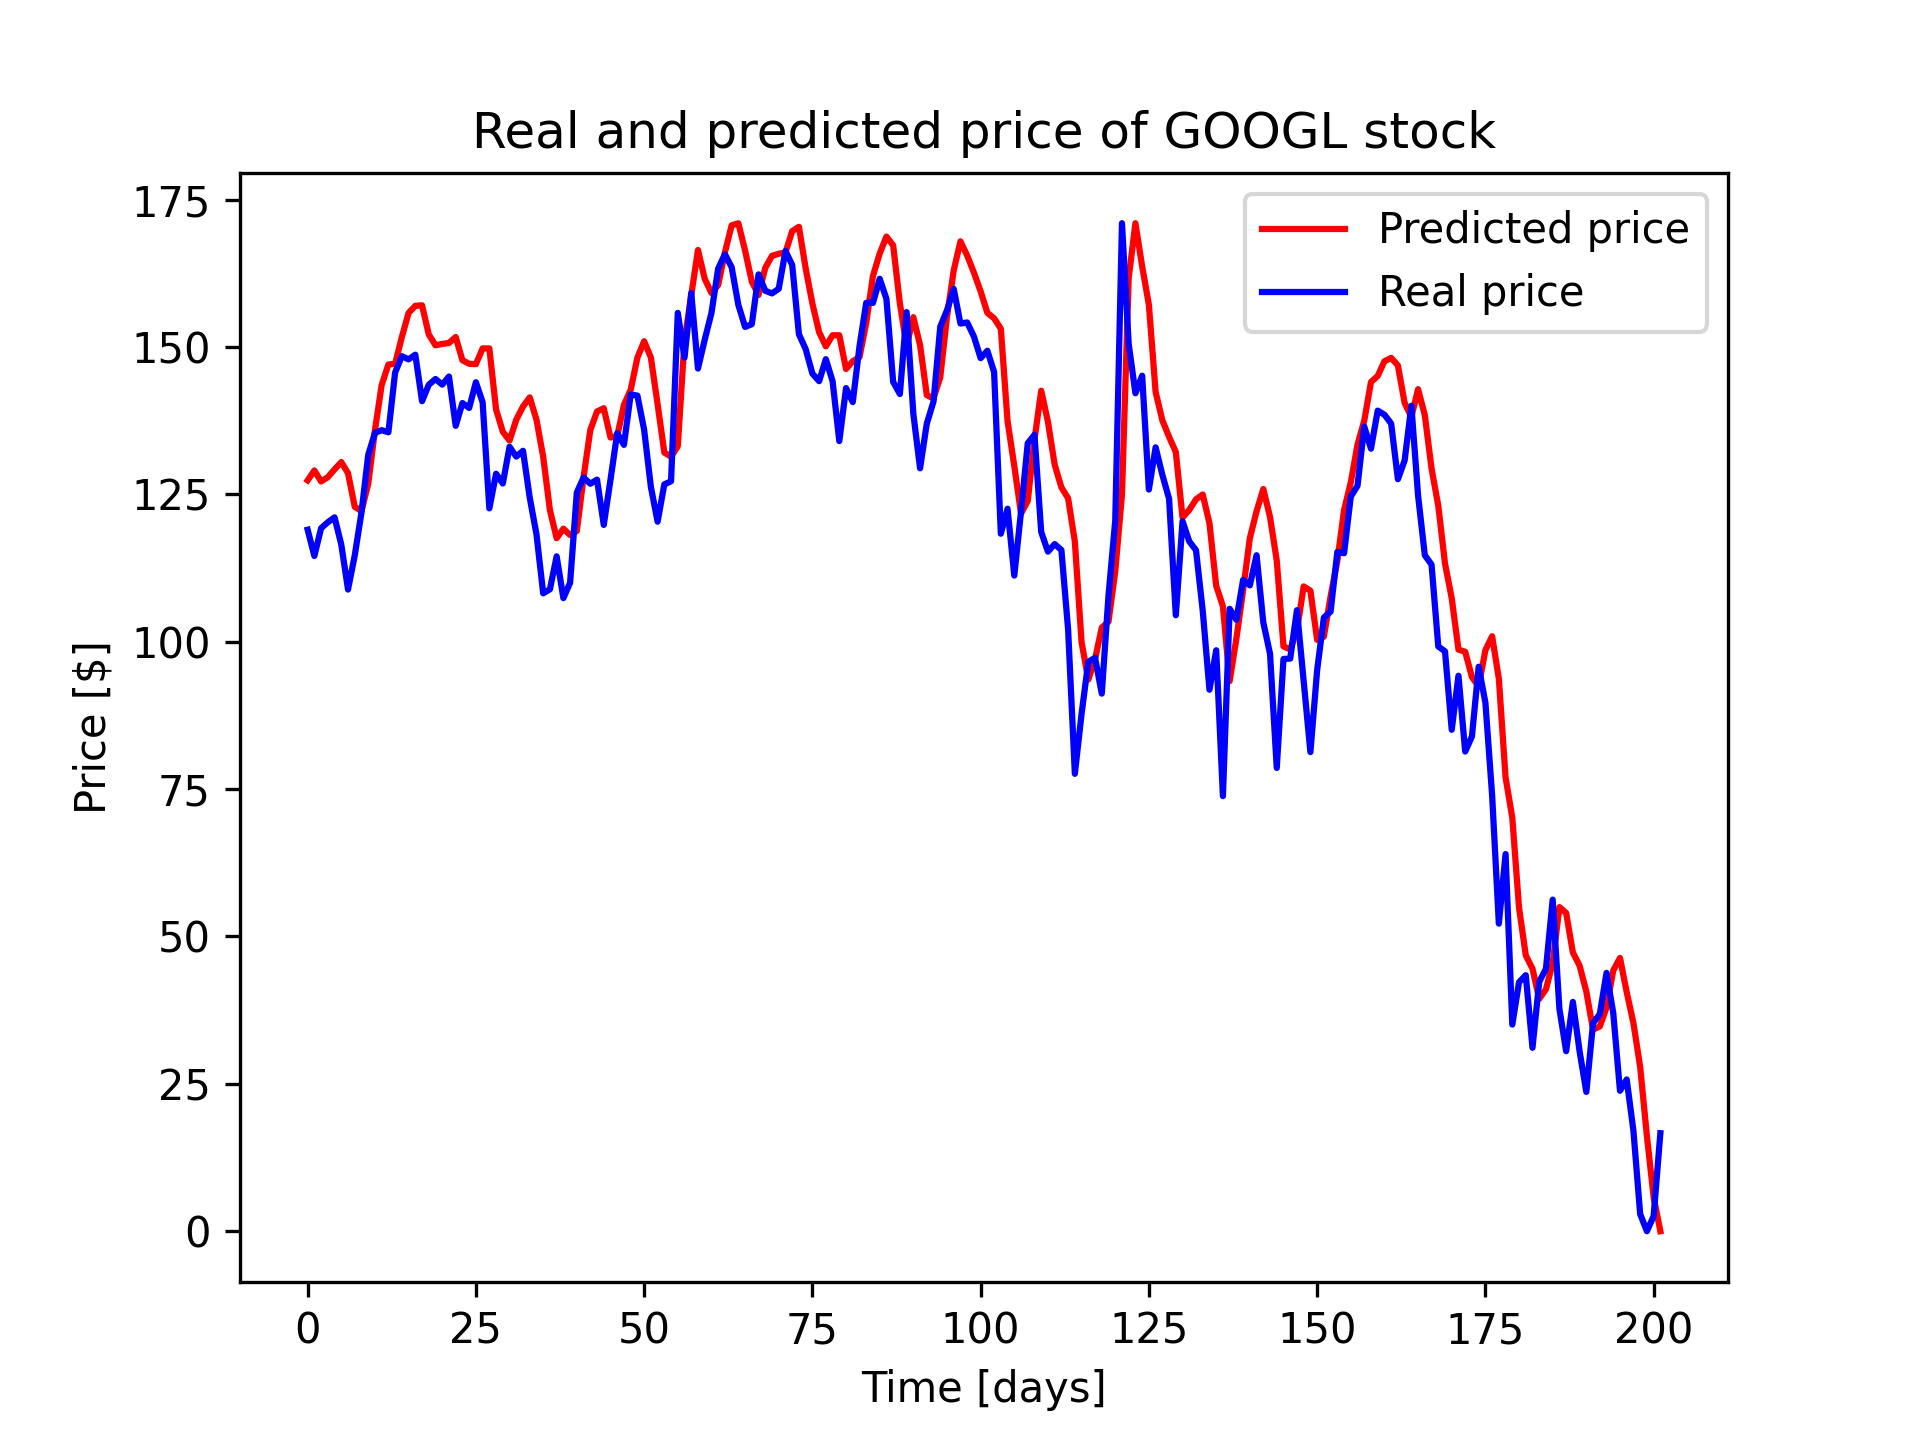
\includegraphics[width=0.5\textwidth]{./graf/model6/GOOGL.png}
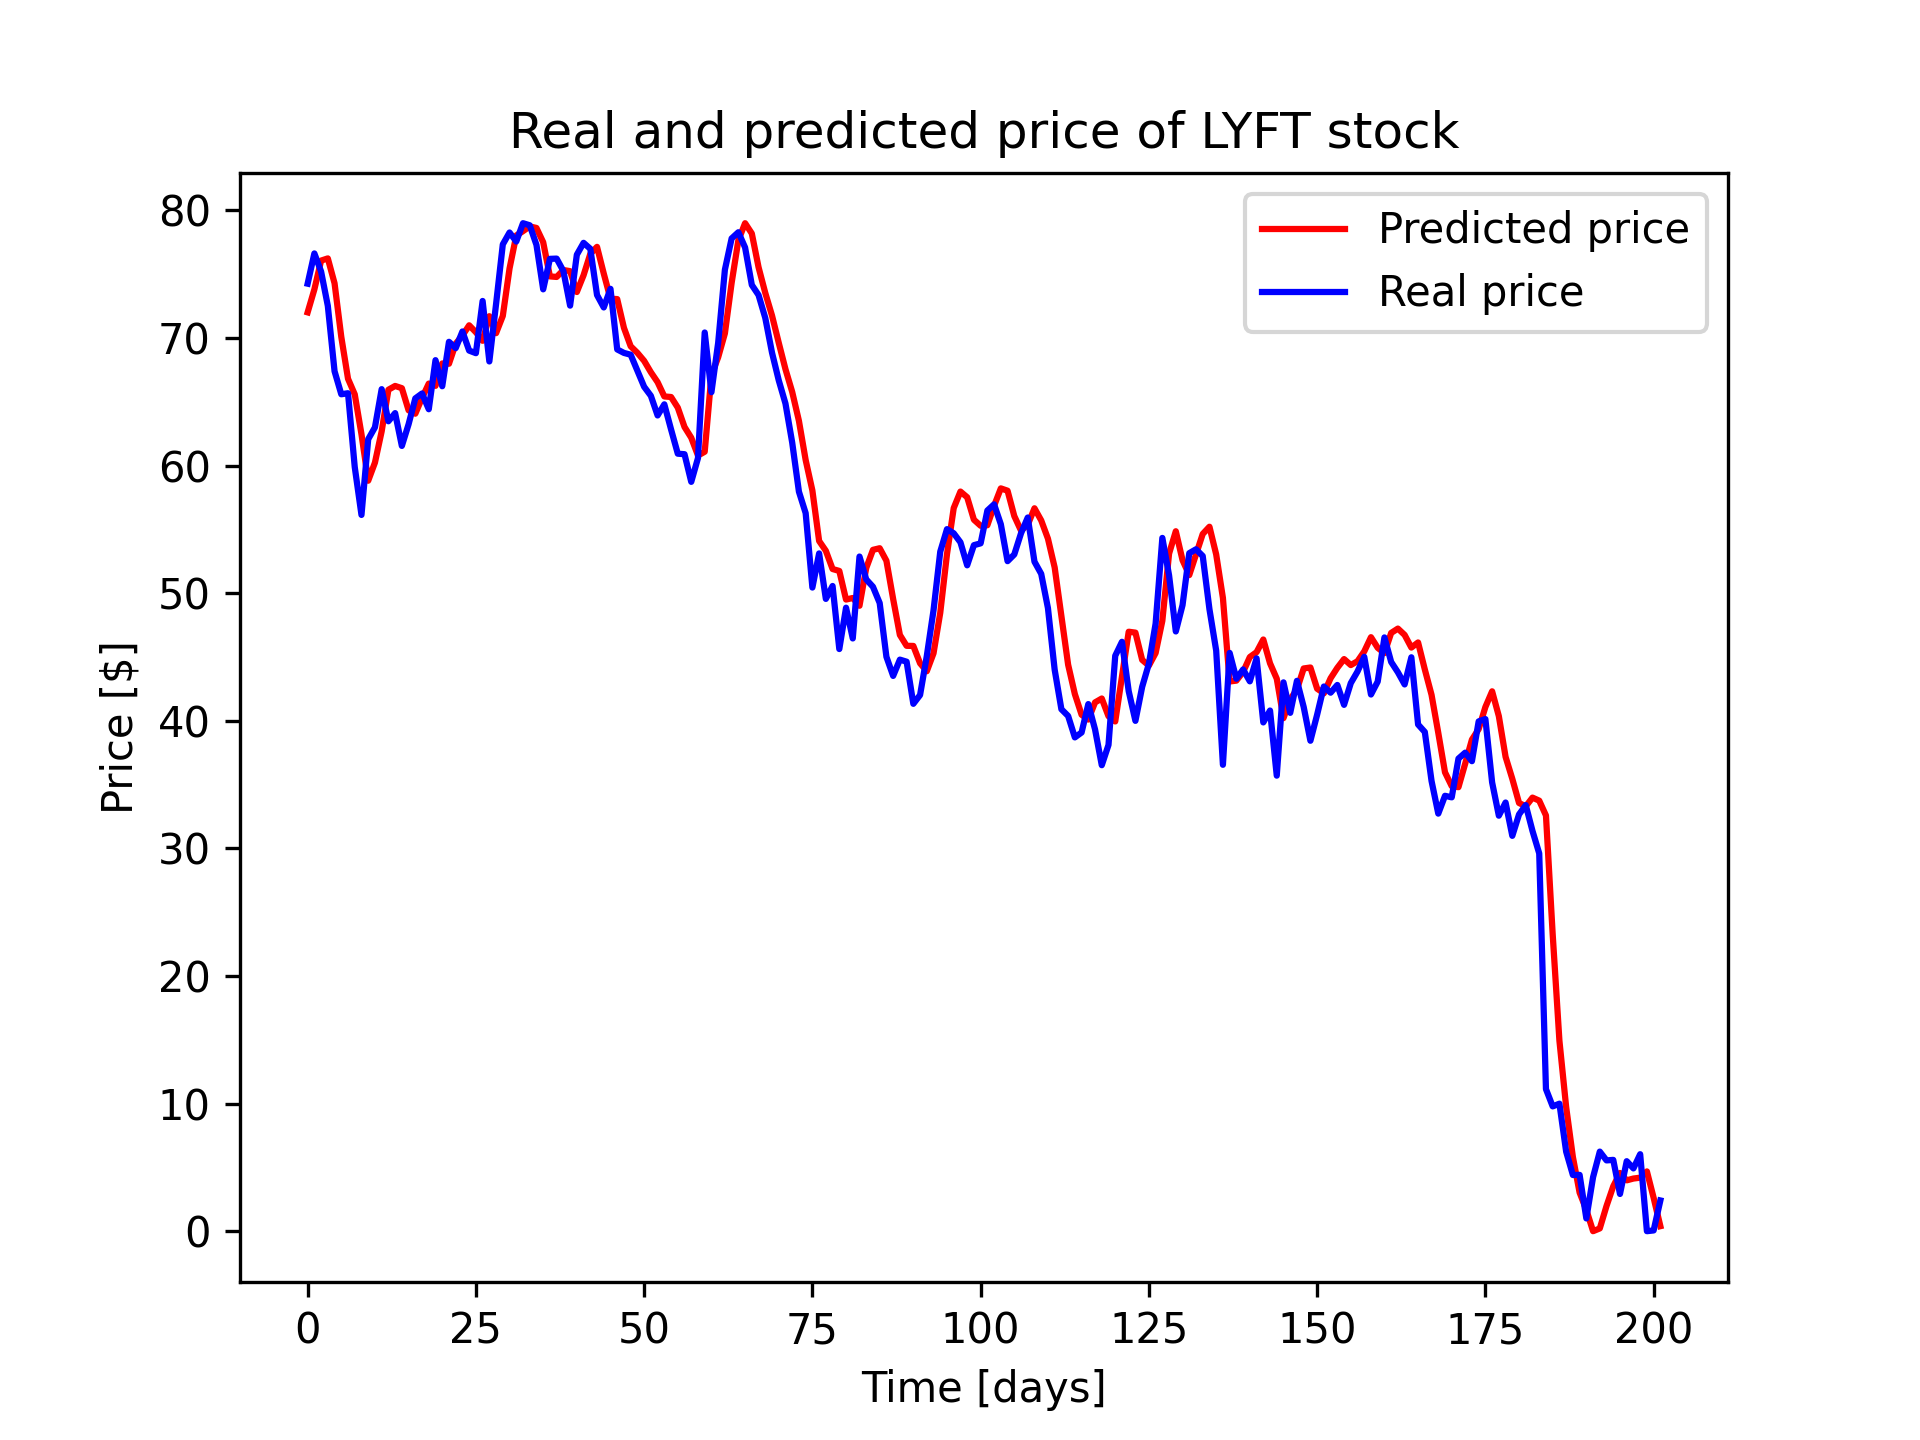
\includegraphics[width=0.5\textwidth]{./graf/model6/LYFT.png}
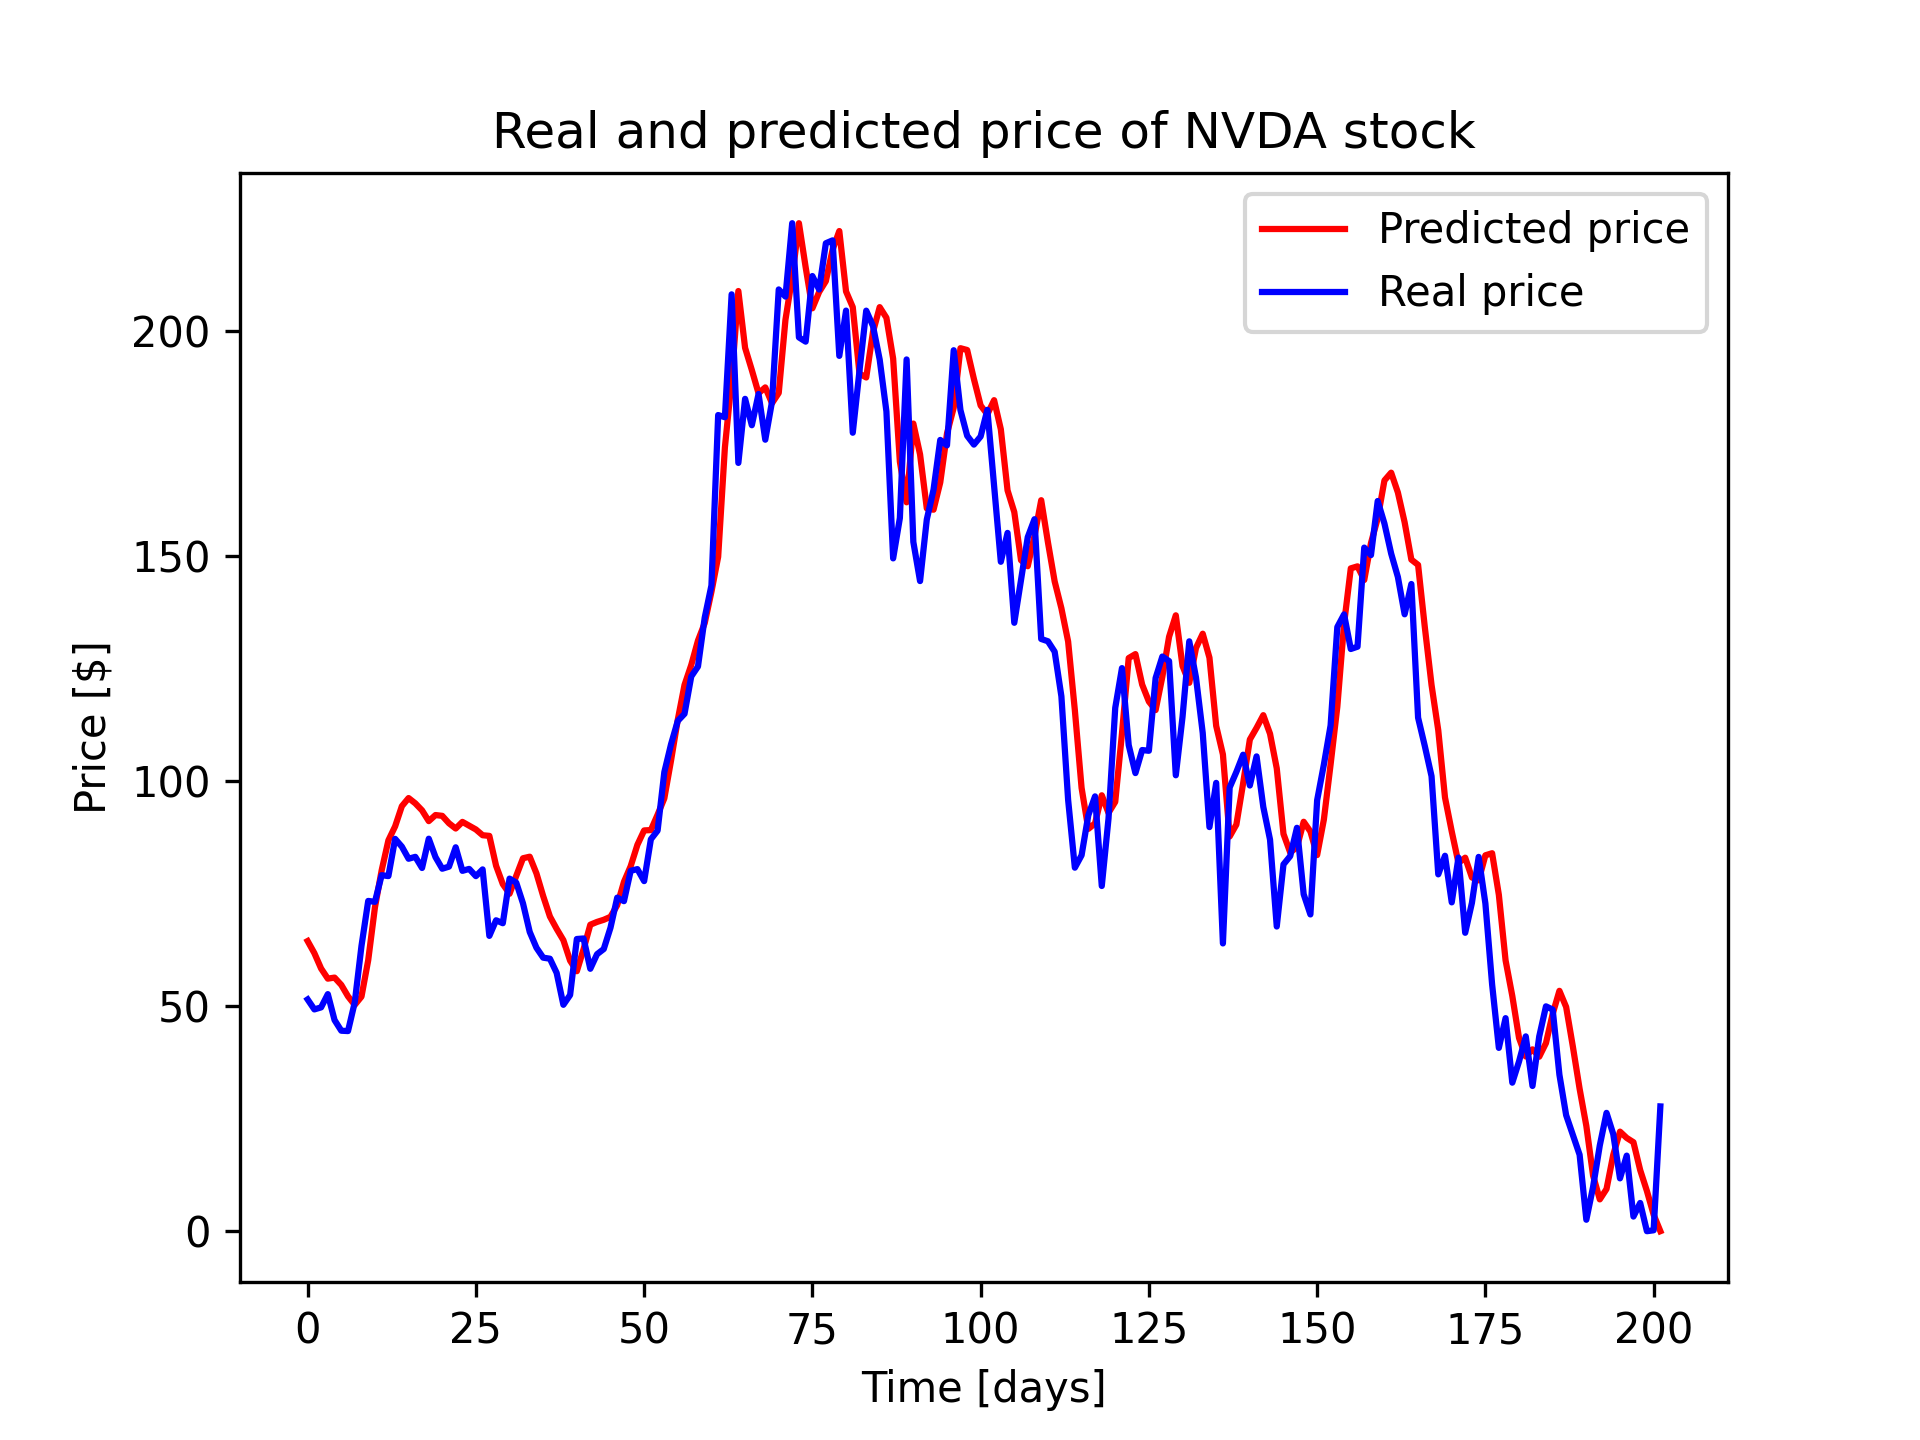
\includegraphics[width=0.5\textwidth]{./graf/model6/NVDA.png}
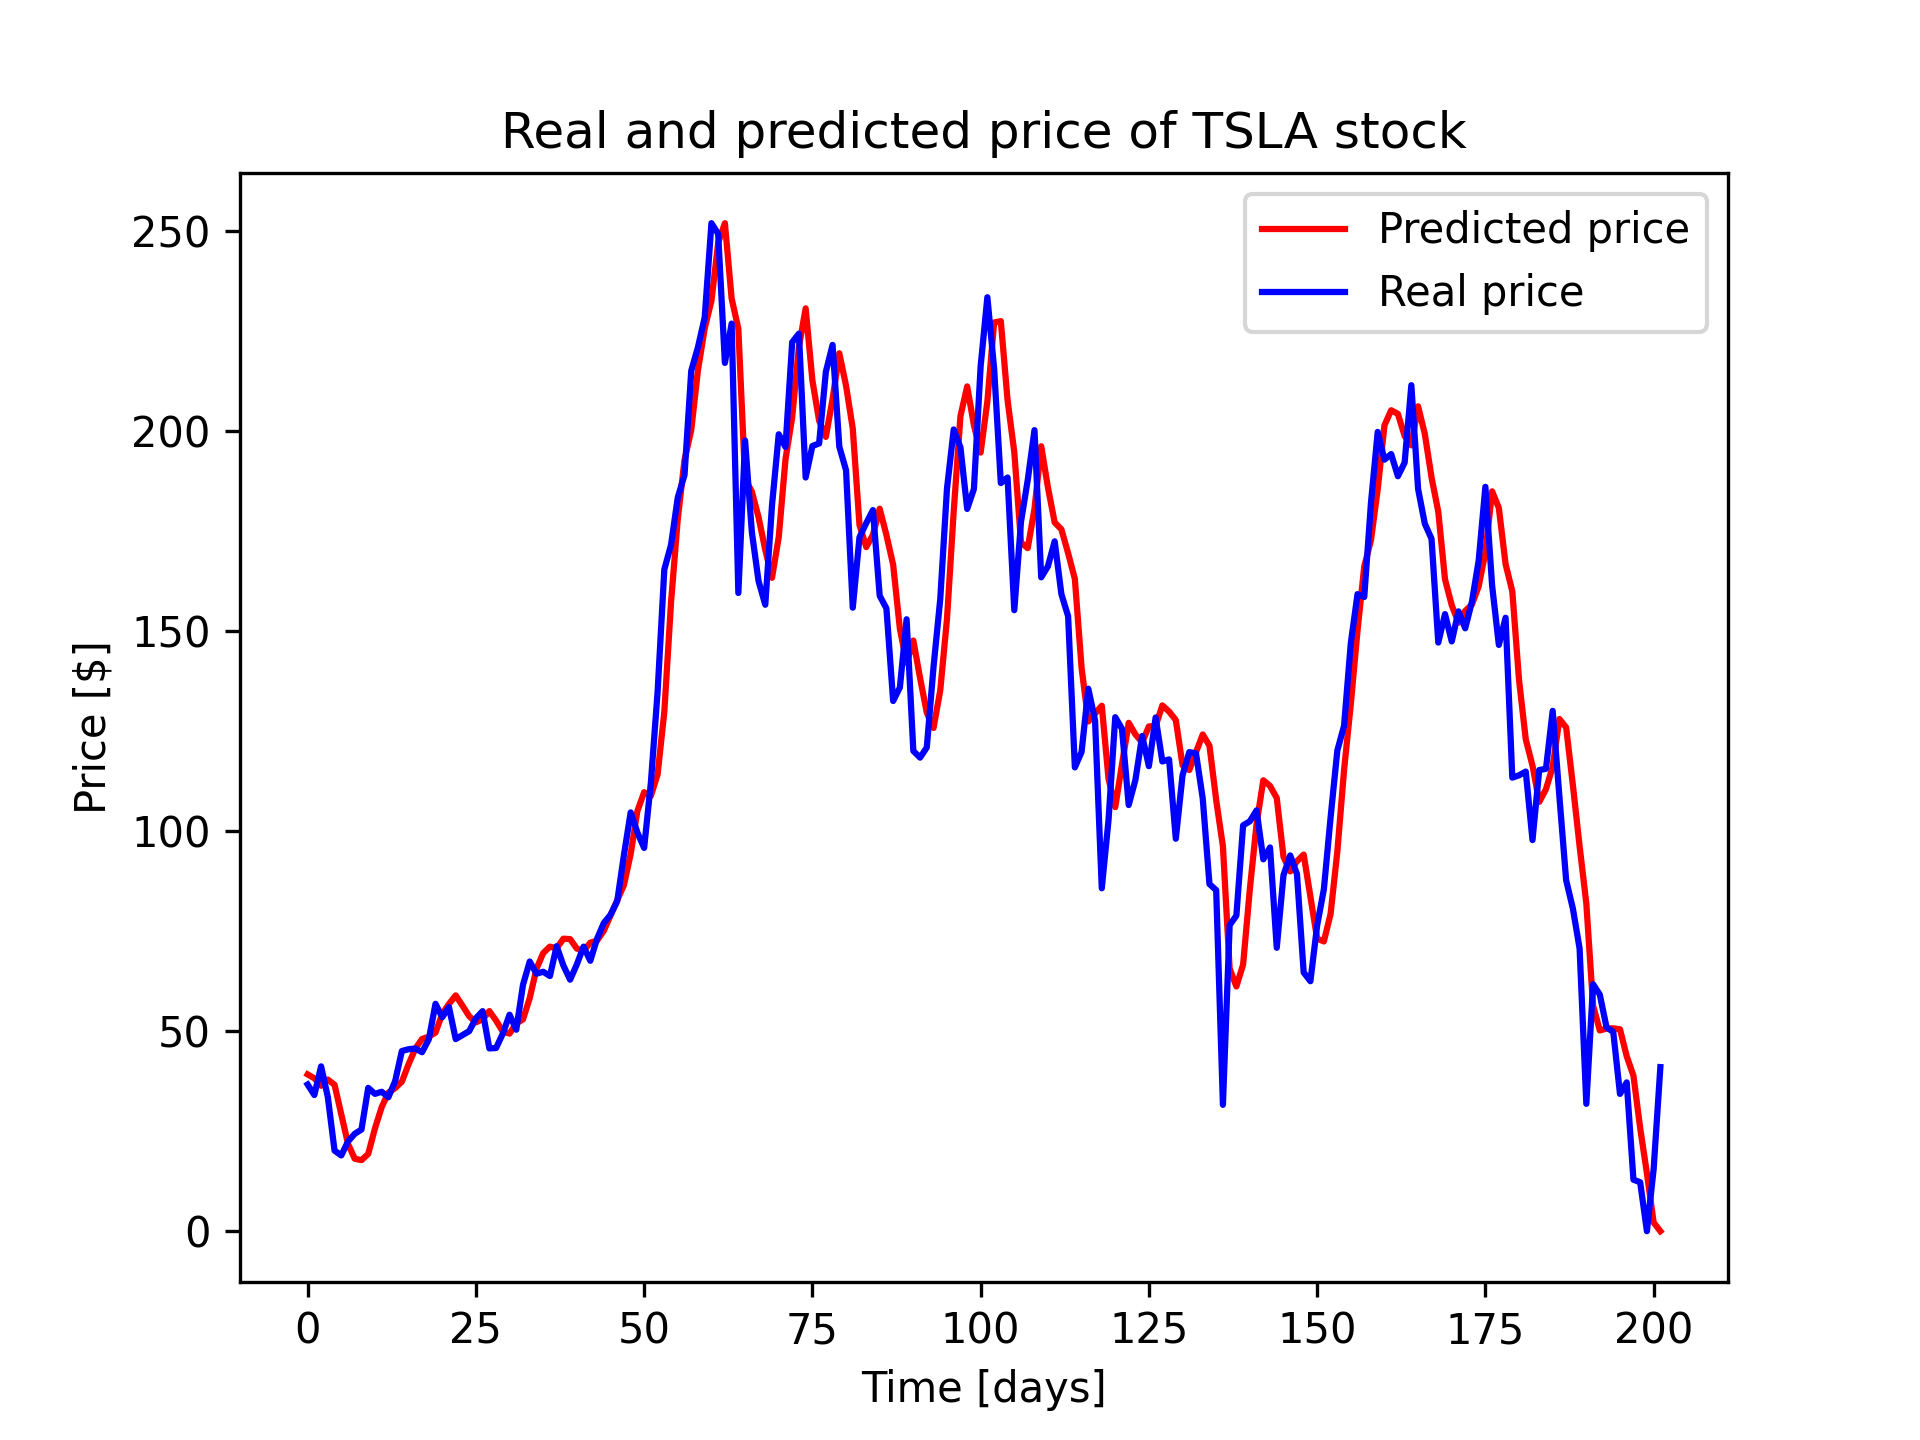
\includegraphics[width=0.5\textwidth]{./graf/model6/TSLA.png}
\caption{Real and predicted prices of the sixth model.}
\label{fig:label}
\end{figure} 

\clearpage
\subsection{Model 7}

Model7 - chunkSize: 100, time interval: 1 year, epochs: 5, trained on AAPL\par\bigskip
In this model, when observing and analyzing the course of both lines, the first thing that can be
noticed is that the red line is too smooth concerning the blue line. The blue line has strongly
peaked peaks, while the red line is visibly smooth throughout its course. Only a mild increase or
decrease in prices is signaled. In this model, short-term price fluctuations were not marked on the
charts. Few-day discounts or increases are not reflected in the red line. Sudden, rapid
changes are not included in this model. In addition, the red line is significantly shifted to the right and
runs higher than the blue line for its entire length.

\begin{figure}
% \centering
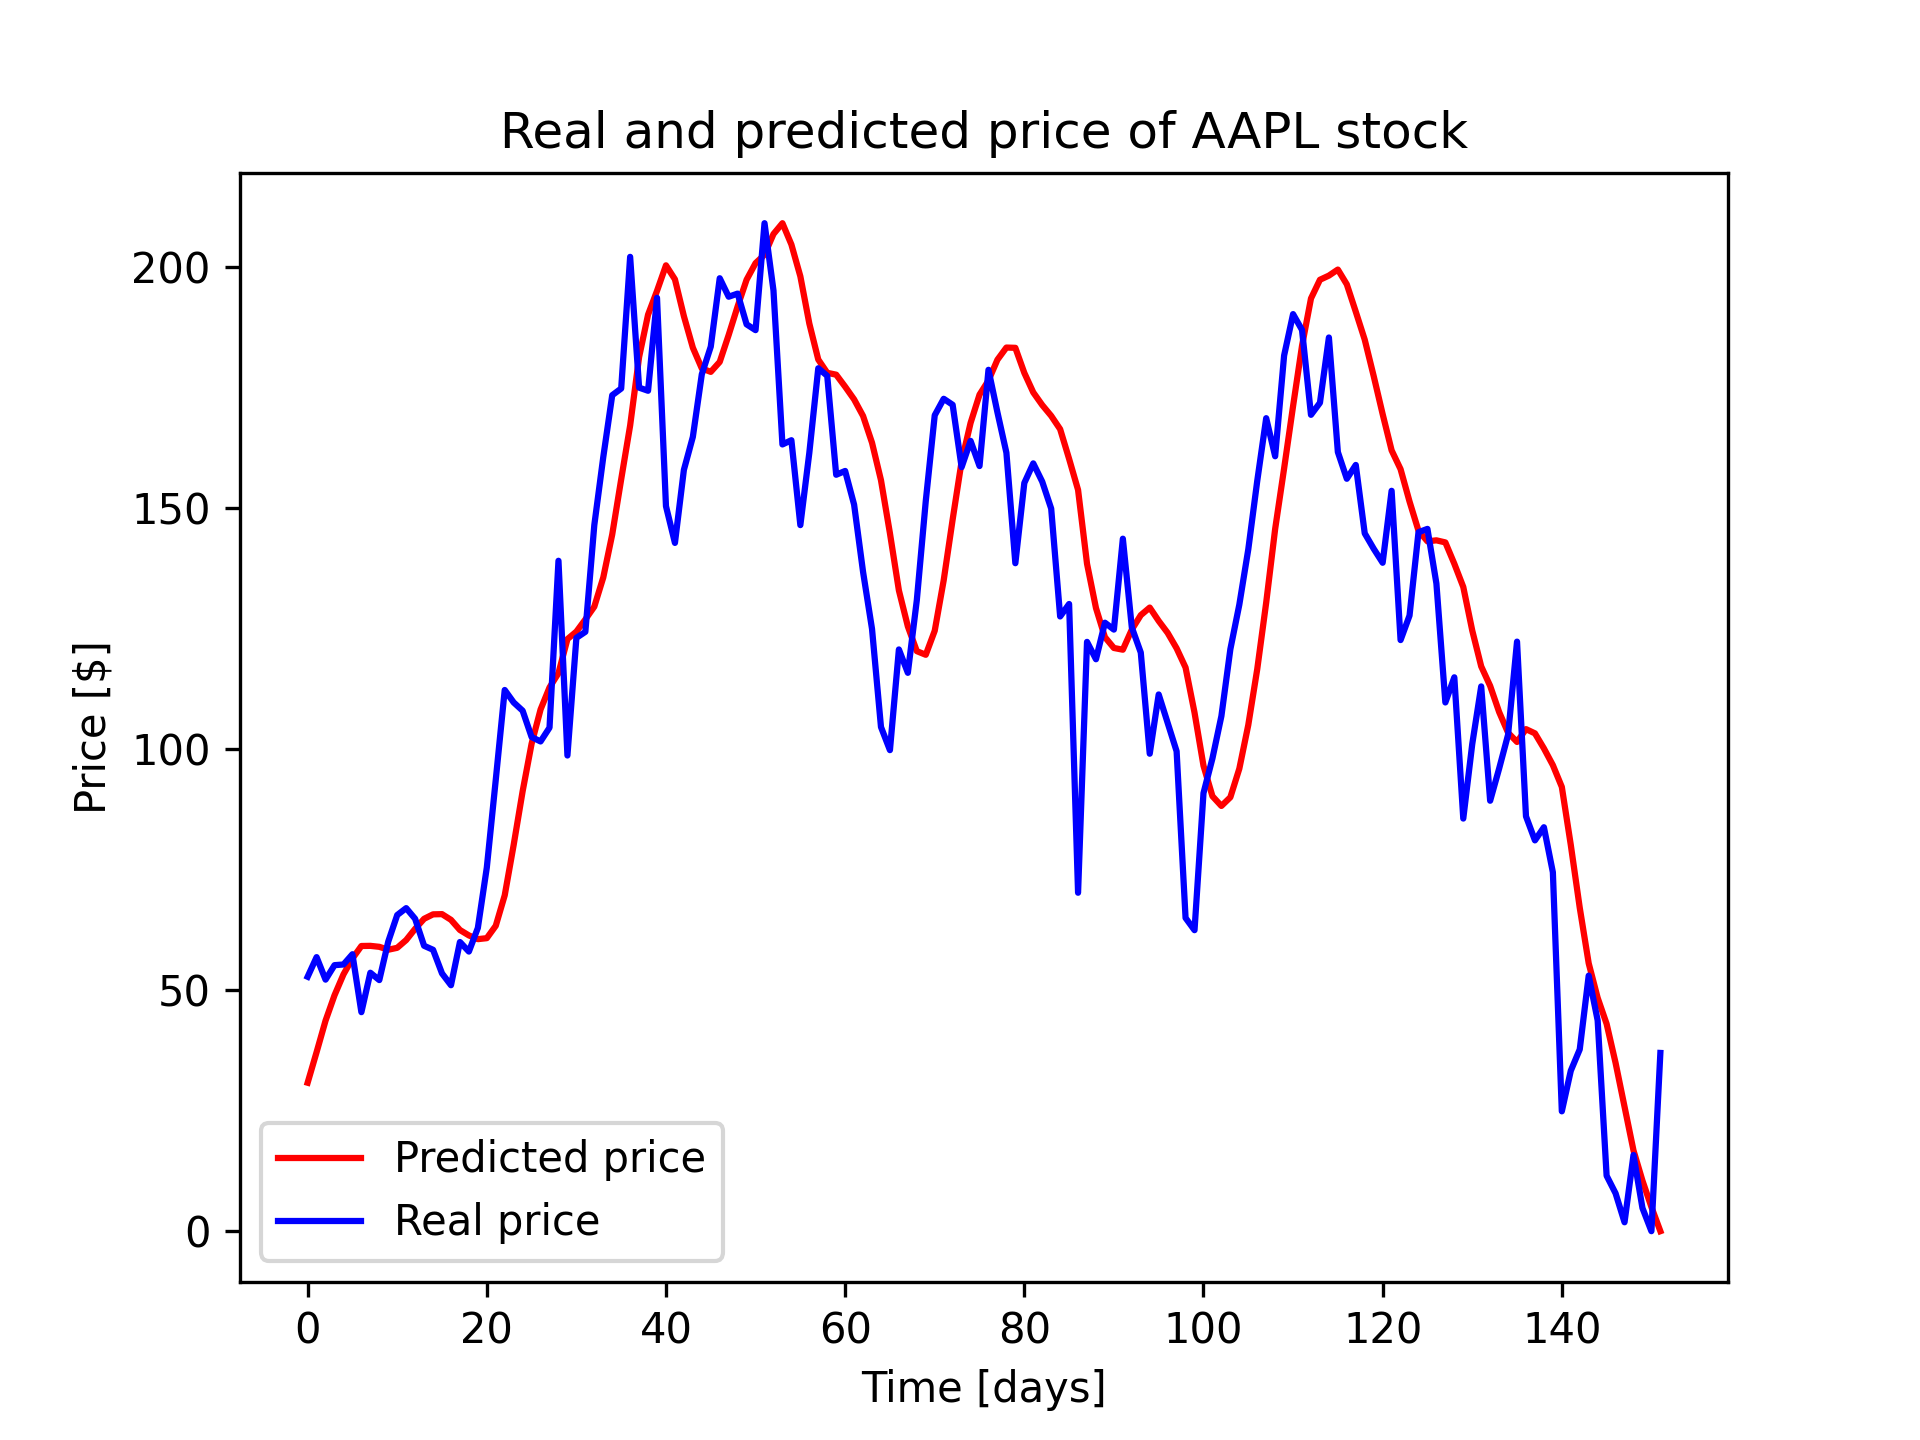
\includegraphics[width=0.5\textwidth]{./graf/model7/AAPL.png}
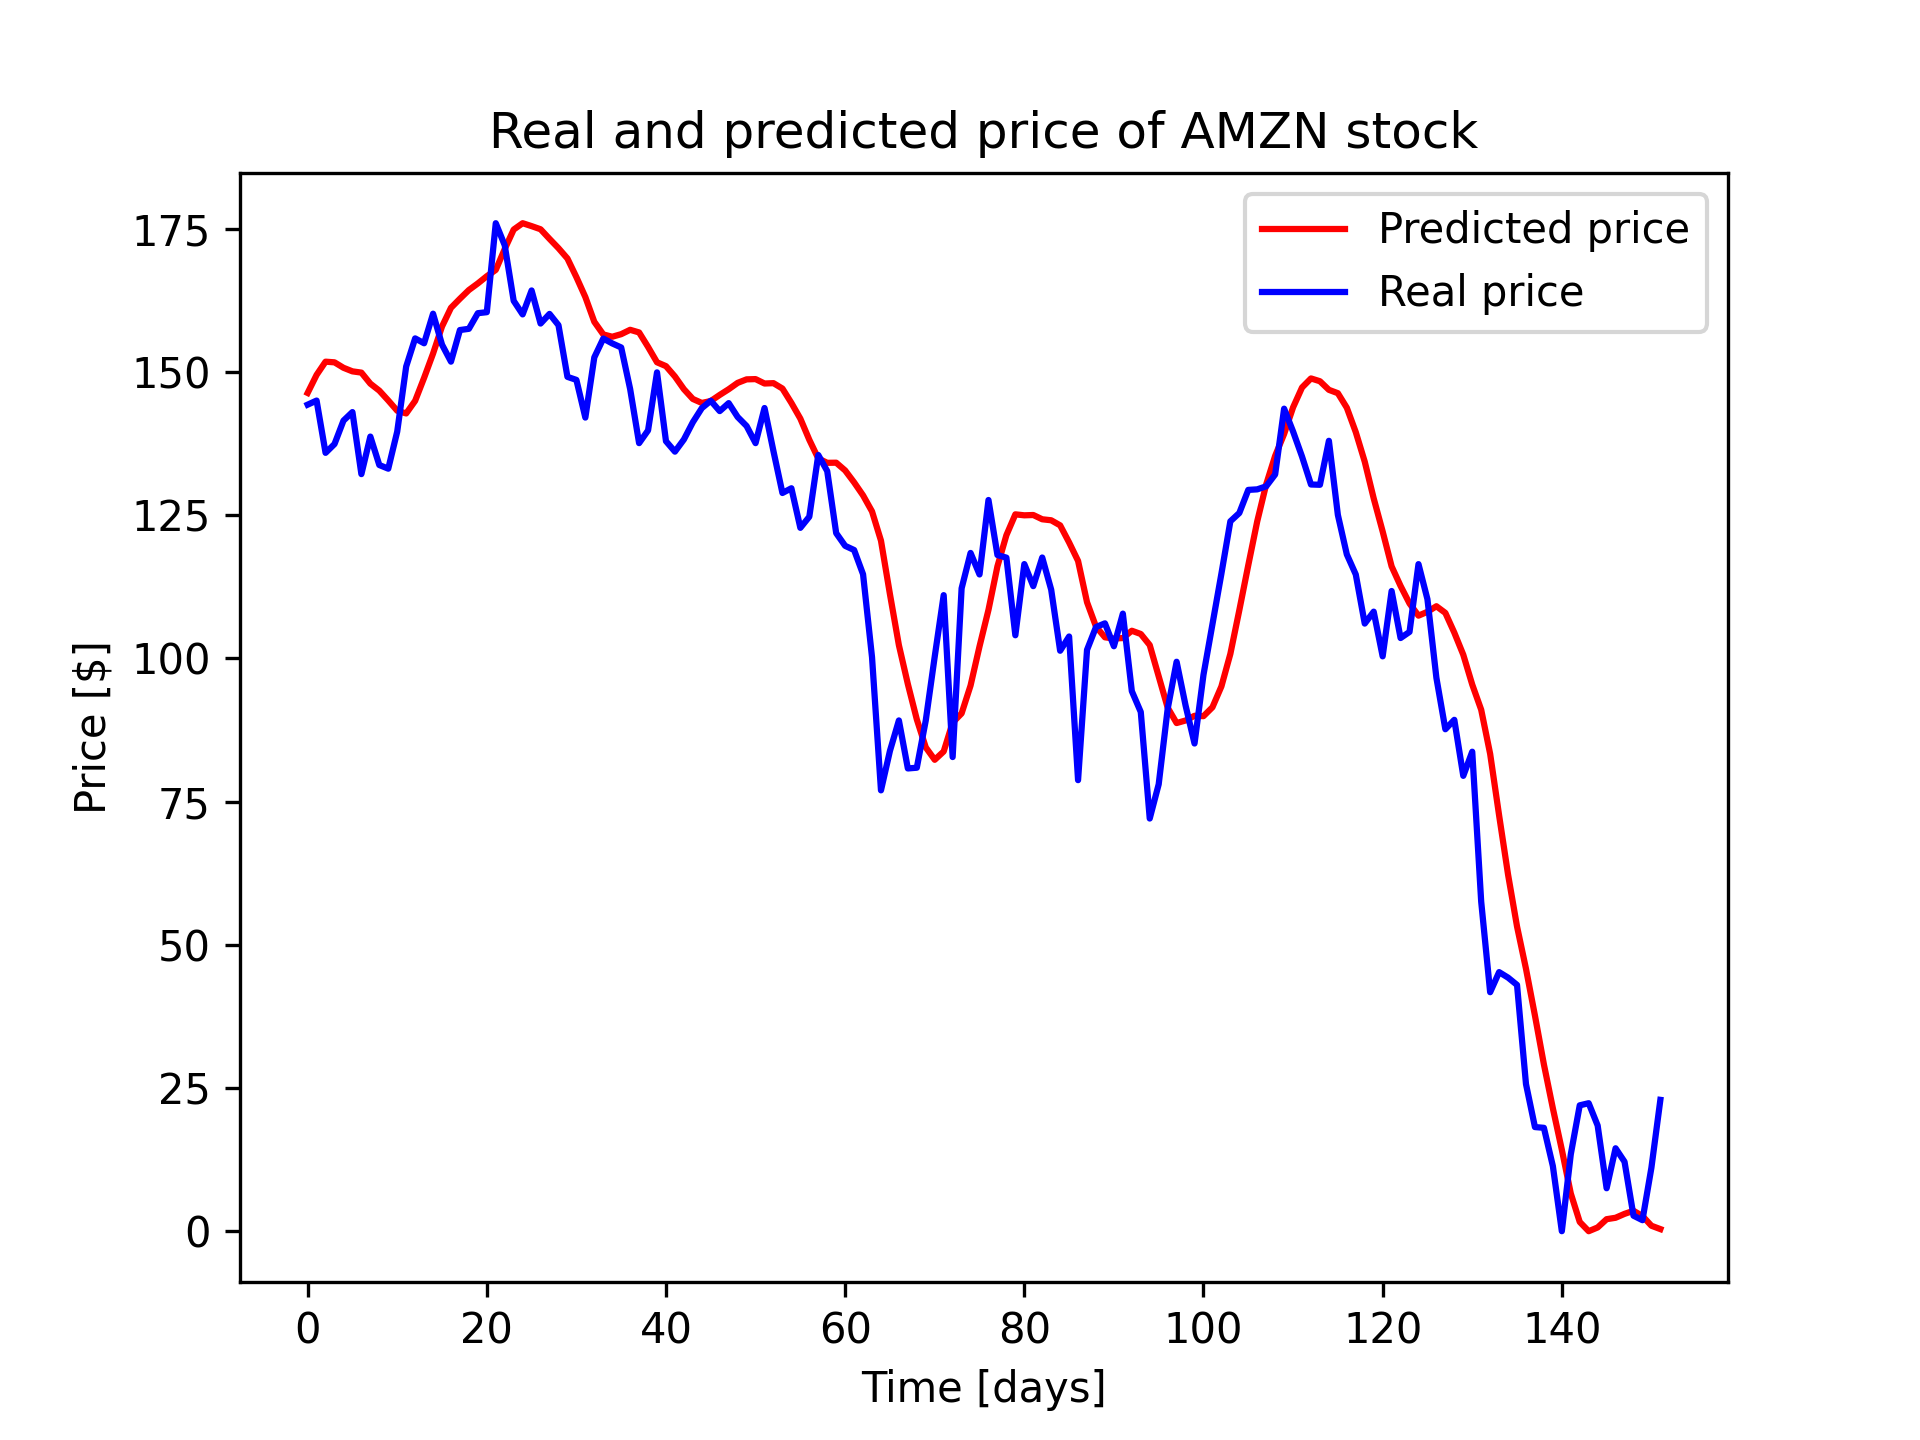
\includegraphics[width=0.5\textwidth]{./graf/model7/AMZN.png}
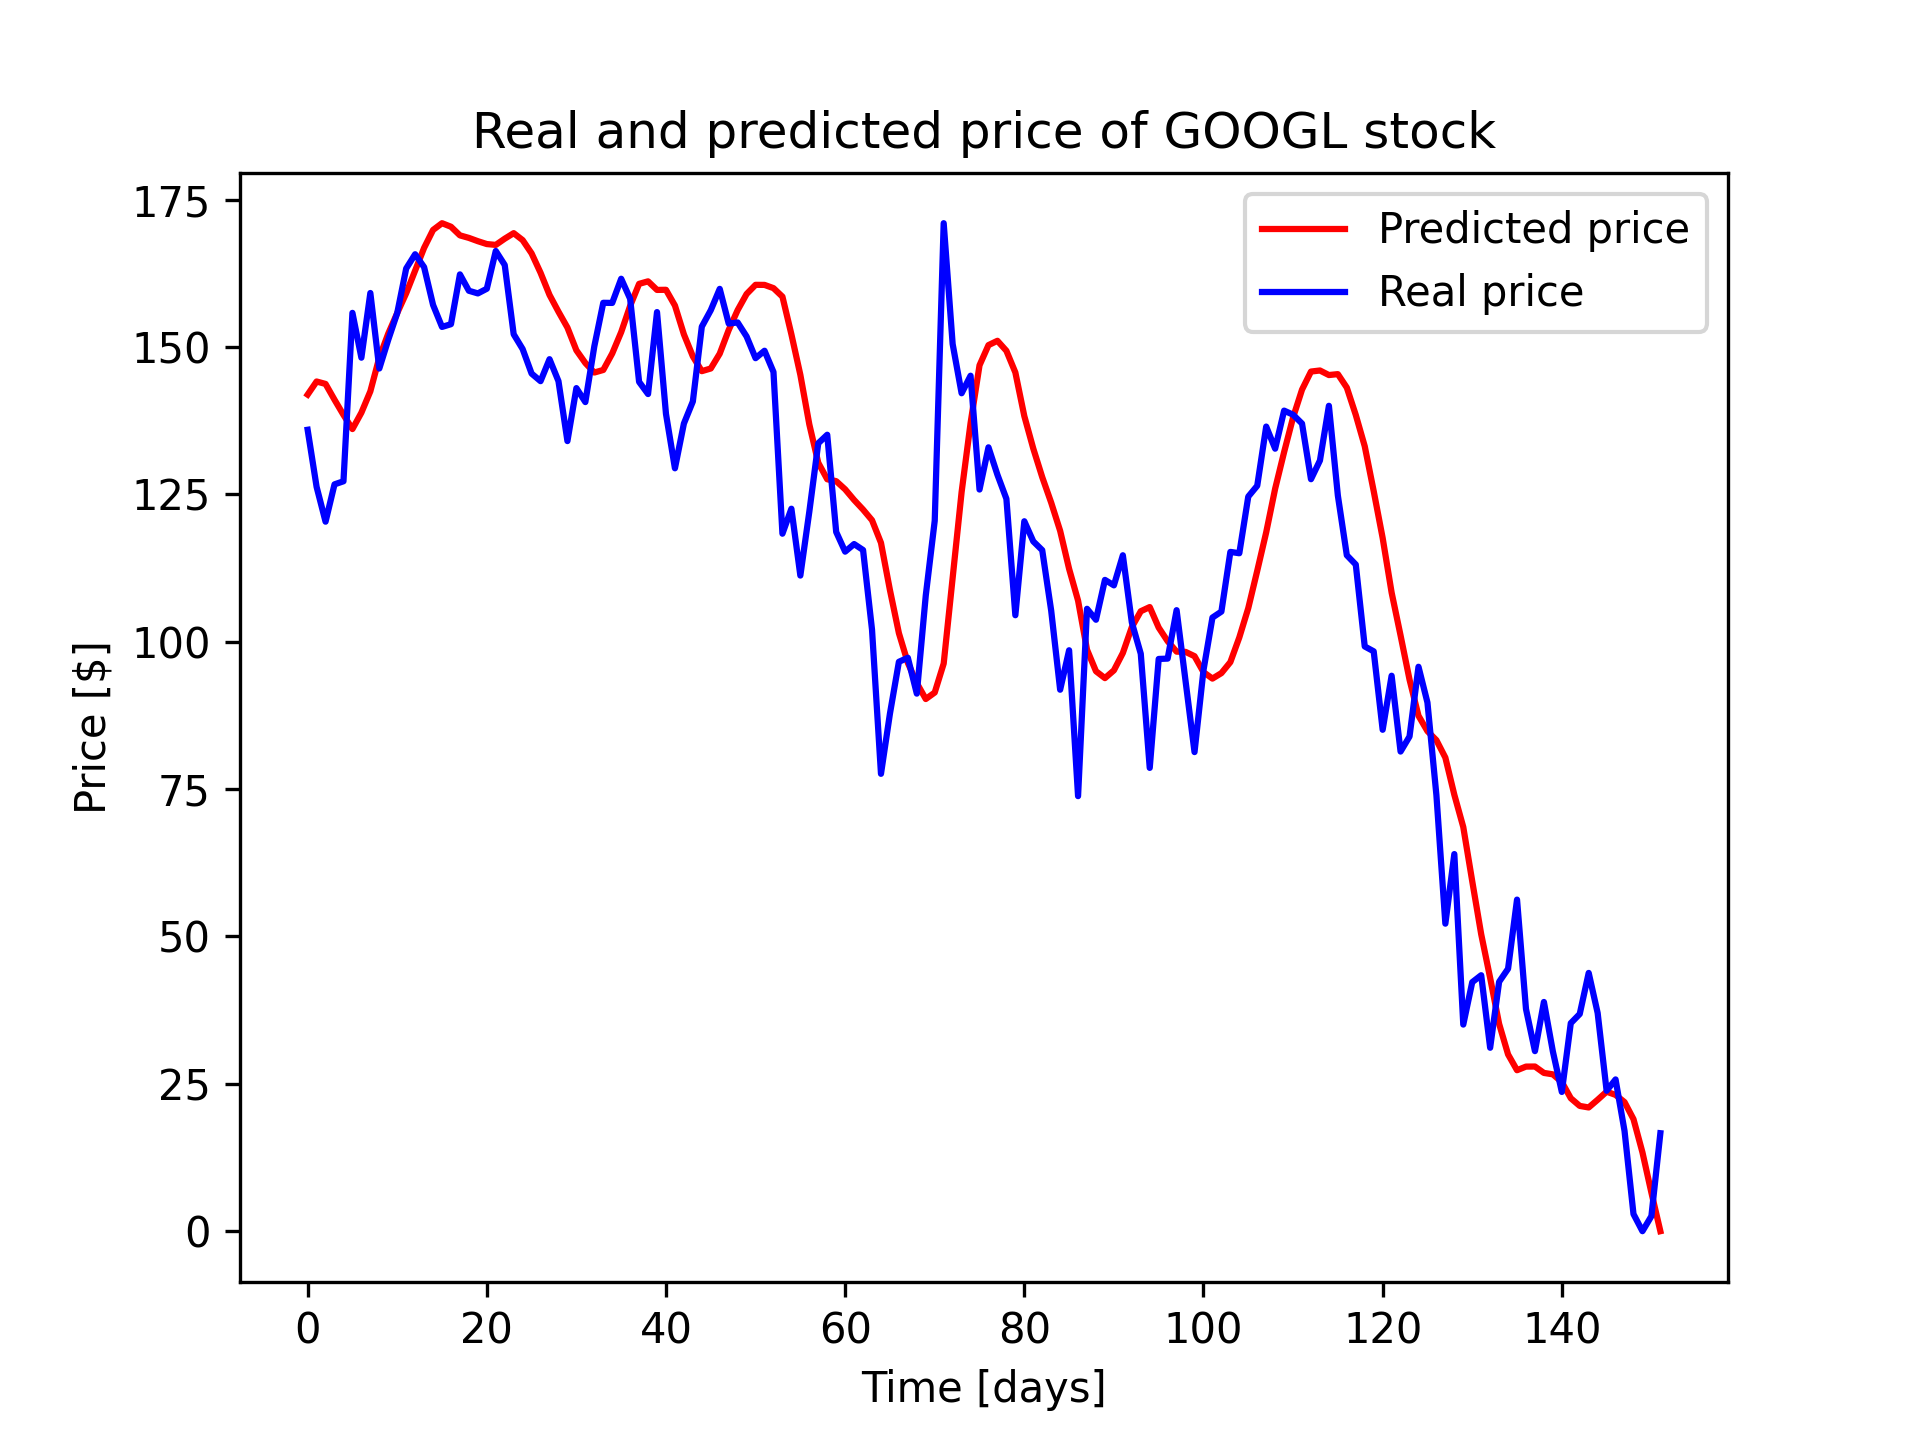
\includegraphics[width=0.5\textwidth]{./graf/model7/GOOGL.png}
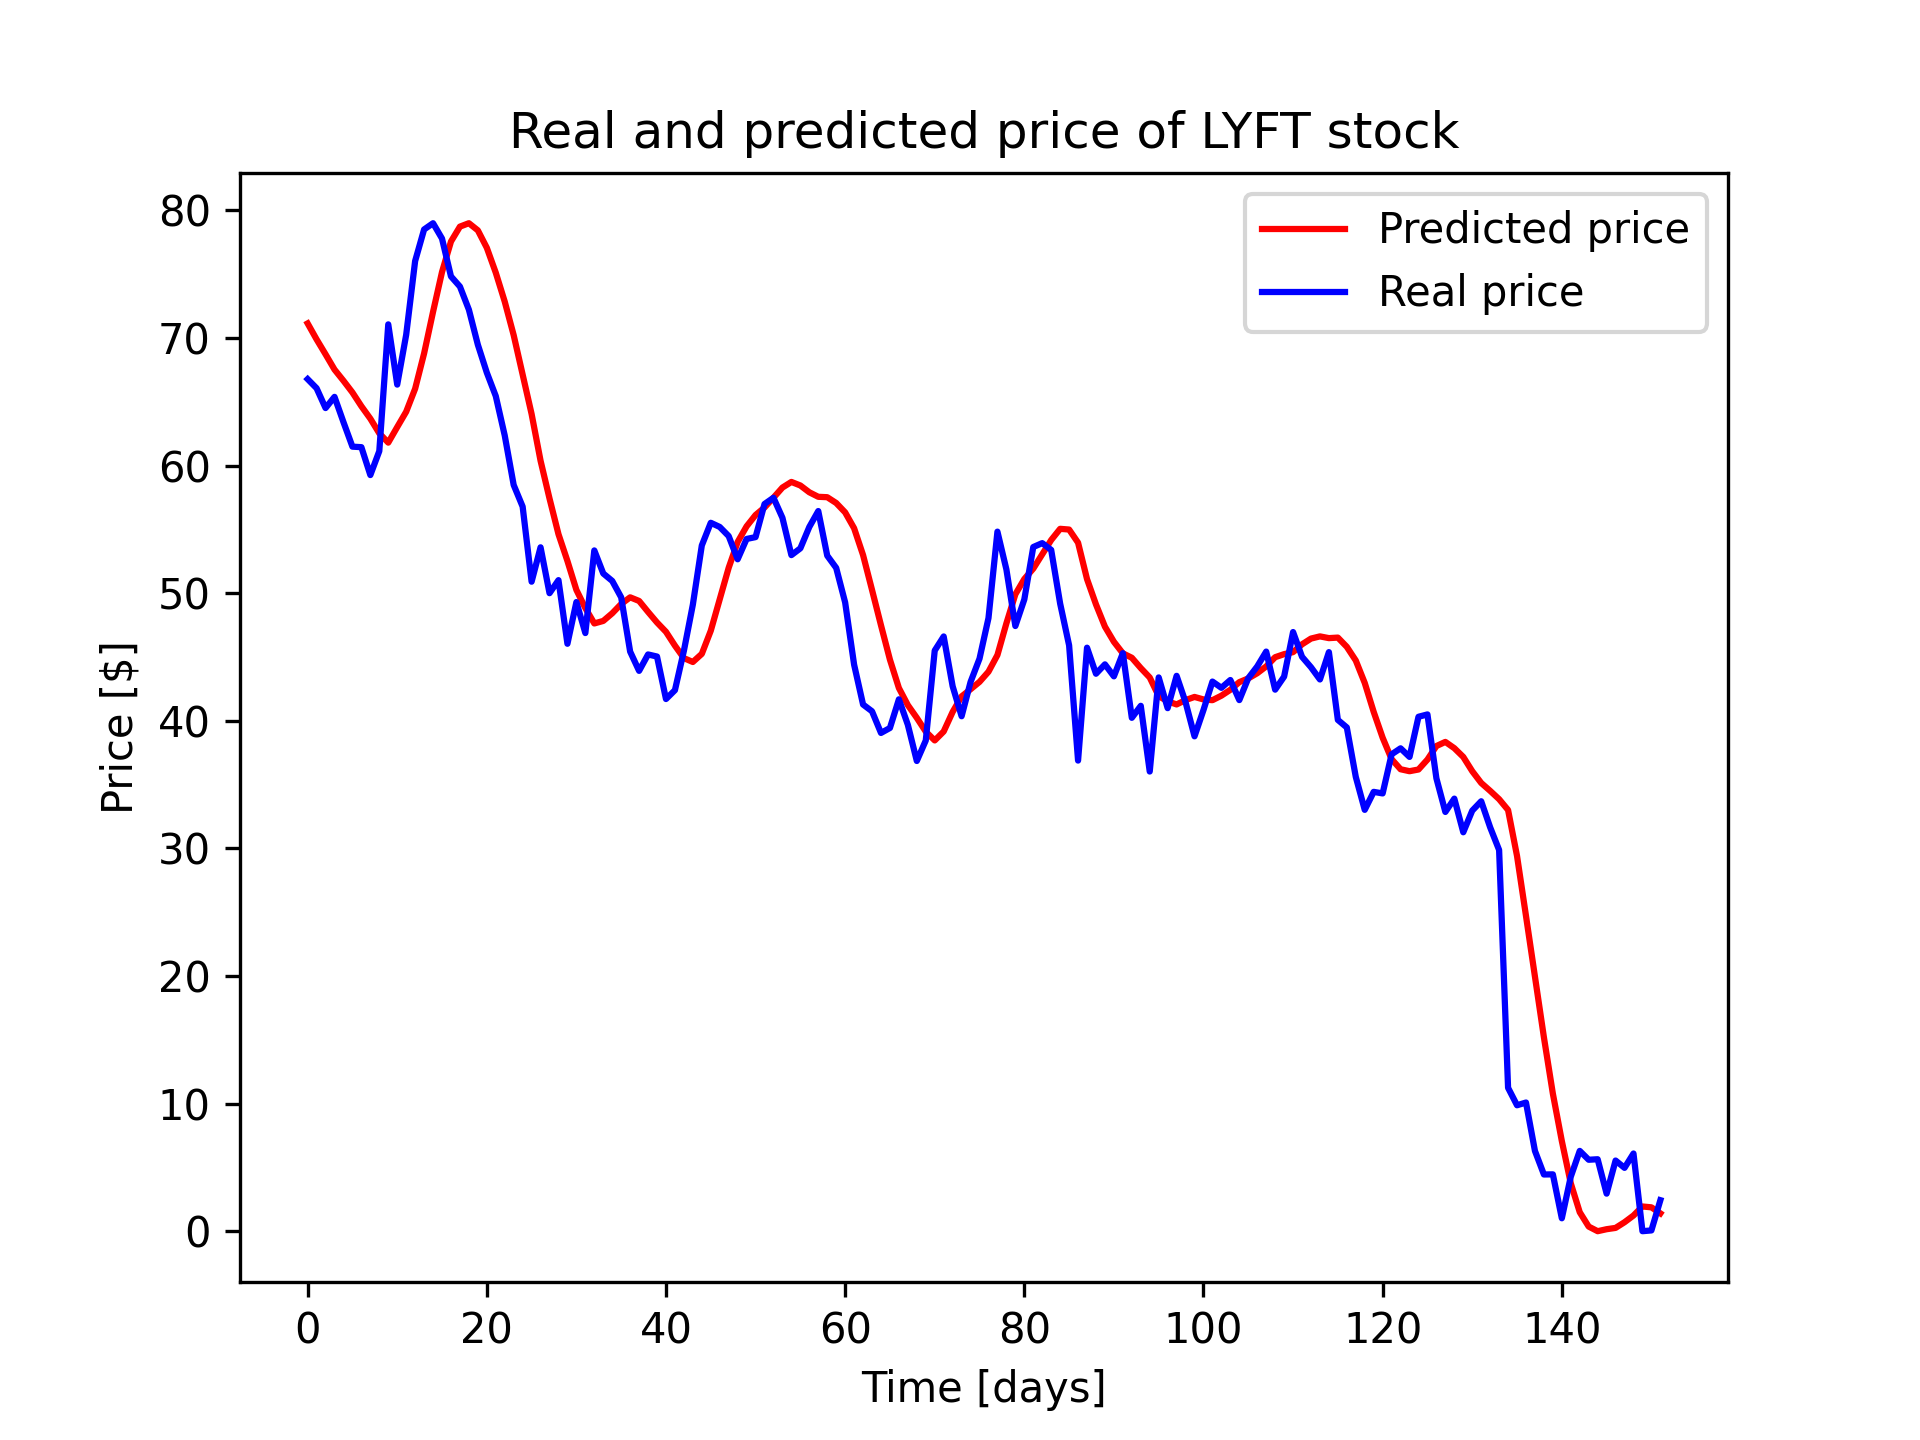
\includegraphics[width=0.5\textwidth]{./graf/model7/LYFT.png}
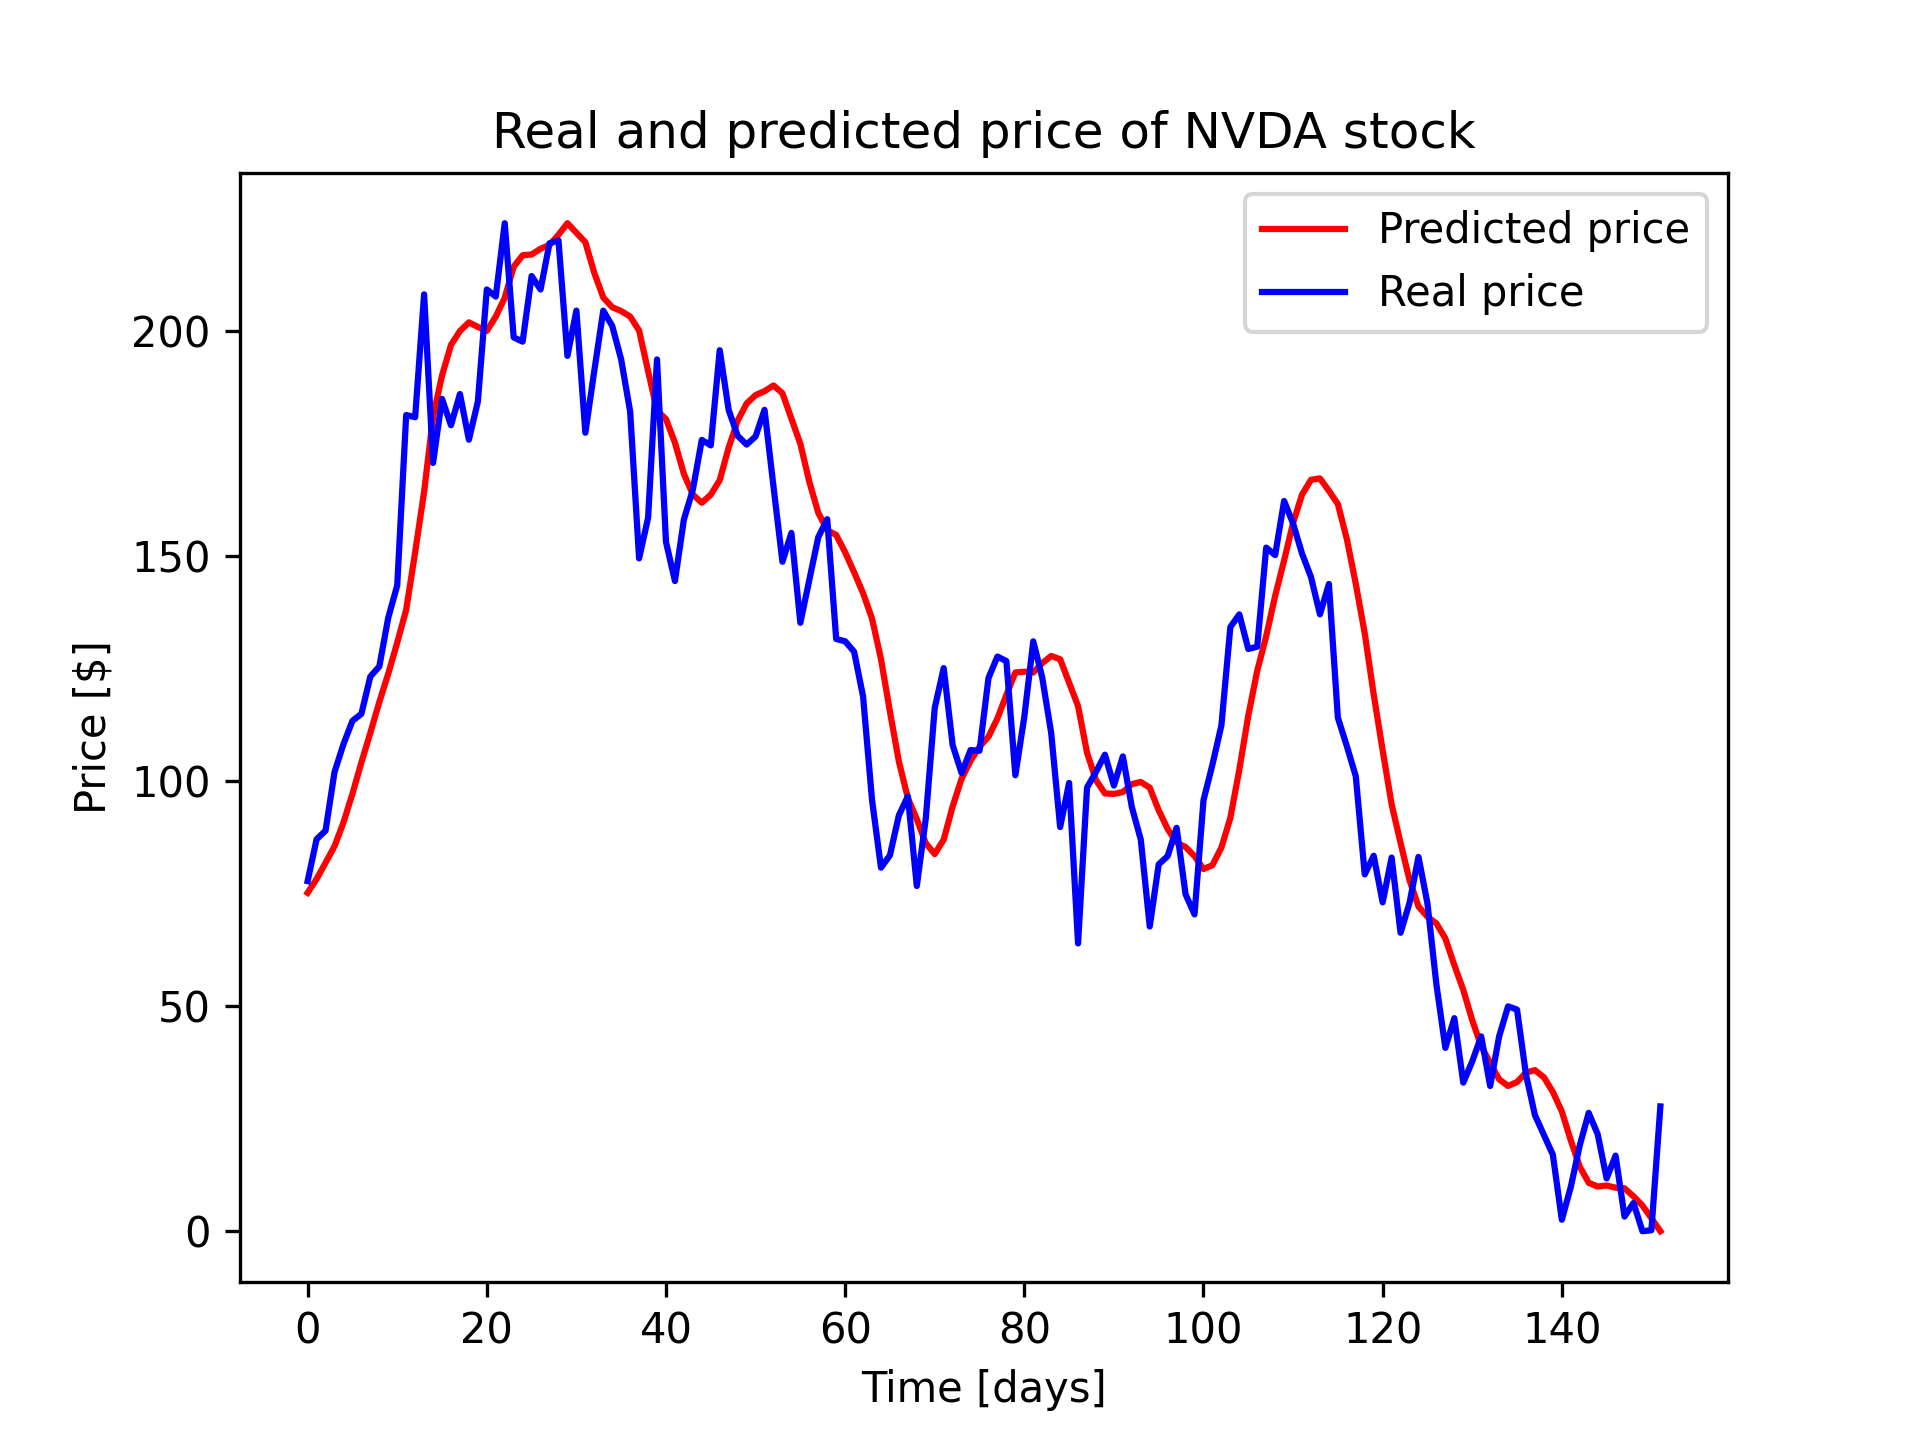
\includegraphics[width=0.5\textwidth]{./graf/model7/NVDA.png}
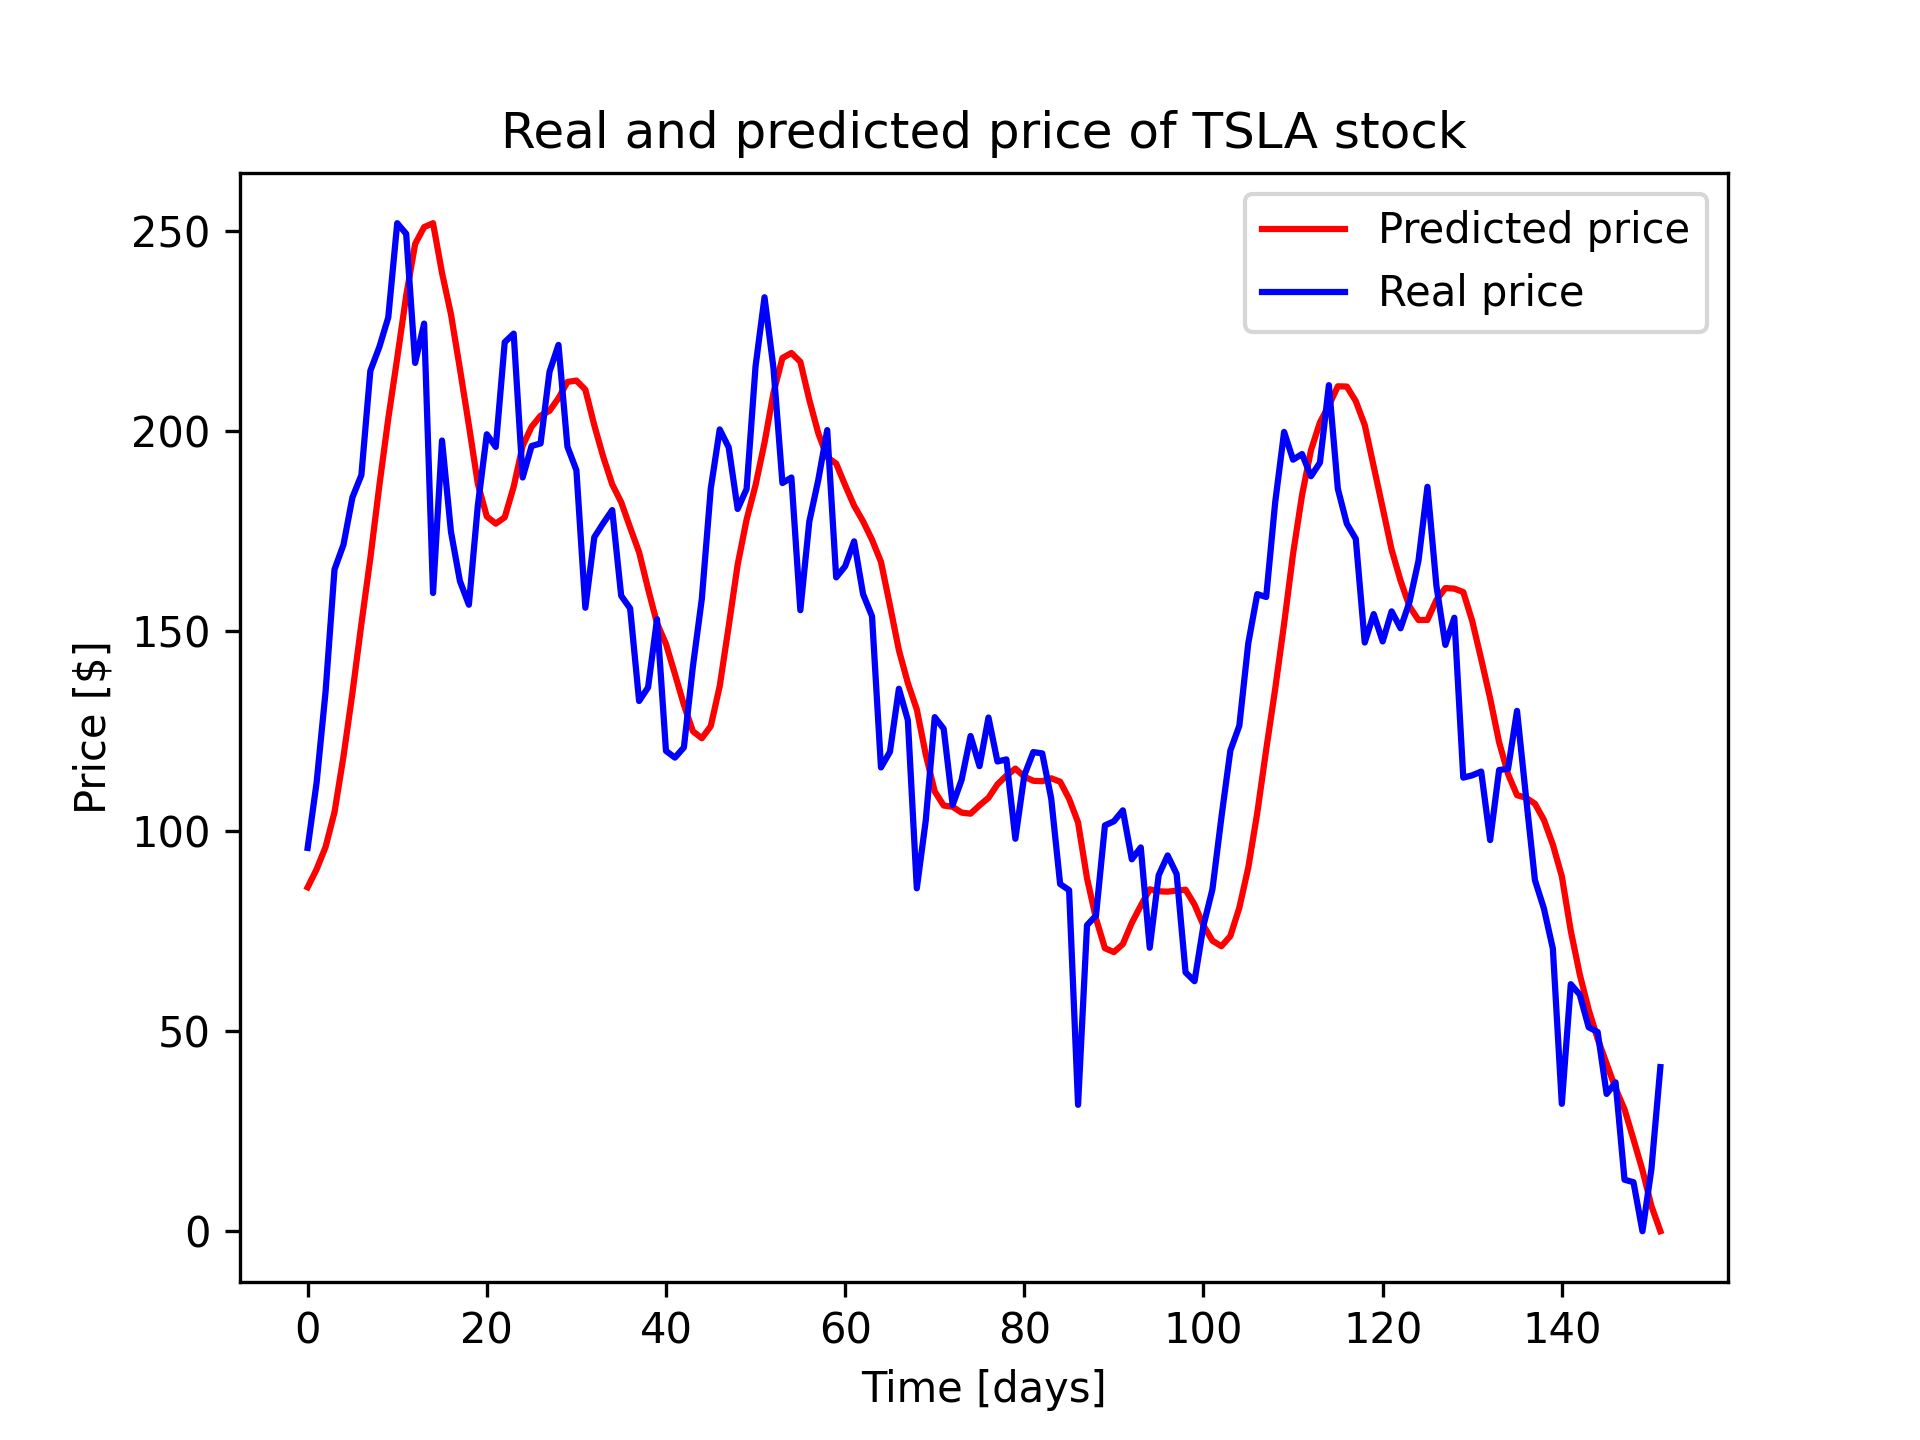
\includegraphics[width=0.5\textwidth]{./graf/model7/TSLA.png}
\caption{Real and predicted prices of the seventh model.}
\label{fig:label}
\end{figure} 

\clearpage
\subsection{Model 8}

Model8 - chunkSize: 100, time interval: 1 year, epochs: 10, trained on AAPL\par\bigskip
In the graphs of this model, one can observe the shift of the red line upwards relative to the blue line.
The general route of the two lines does not coincide, however, it reflects the general tendency to
increase or decrease prices. Rapid price drops are signaled by a blue line, for example, in the chart for AAPL.png.,
and GOOGL.png. they are not reflected in the course of the blue line. The same is true in two cases of
a sudden one-day price increase, as in the charts for GOOGL.png., and NVDA.png.,
however, in these cases, the blue line peaks do not go much above the red line. In addition, the red
line has a much more gentle course compared to the blue line, and it is flattened in places with very rapid price changes. What is worth noticing, the long-term systematic progression of
prices is precisely marked, and both lines have an almost identical course.

\begin{figure}
% \centering
\includegraphics[width=0.5\textwidth]{./graf/model8/AAPL.png}
\includegraphics[width=0.5\textwidth]{./graf/model8/AMZN.png}
\includegraphics[width=0.5\textwidth]{./graf/model8/GOOGL.png}
\includegraphics[width=0.5\textwidth]{./graf/model8/LYFT.png}
\includegraphics[width=0.5\textwidth]{./graf/model8/NVDA.png}
\includegraphics[width=0.5\textwidth]{./graf/model8/TSLA.png}
\caption{Real and predicted prices of the eighth model.}
\label{fig:label}
\end{figure} 

\clearpage
\subsection{Model 9}

Model9 - chunkSize: 100, time interval: 1 year, epochs: 15, trained on AAPL\par\bigskip
In this model, both lines have a very similar course in terms of deflection up or to the side. The lines
in the aged places of the charts coincide with each other. One can also see places on the charts
where the lines intersect, but the general trend in the course of the lines shows a consistent picture
of predicting market prices. The longer-lasting, consistent increase in market prices is very well
illustrated in the chart for NVDA.png., GOOGL.png, AAPL.png, and TSLA.png. On the other hand,
sharp one-day price drops reflected in sharply deflected down peaks, for example, TSLA.png or AAPL.png
do not translate into the course of the blue line.

\begin{figure}
% \centering
\includegraphics[width=0.5\textwidth]{./graf/model9/AAPL.png}
\includegraphics[width=0.5\textwidth]{./graf/model9/AMZN.png}
\includegraphics[width=0.5\textwidth]{./graf/model9/GOOGL.png}
\includegraphics[width=0.5\textwidth]{./graf/model9/LYFT.png}
\includegraphics[width=0.5\textwidth]{./graf/model9/NVDA.png}
\includegraphics[width=0.5\textwidth]{./graf/model9/TSLA.png}
\caption{Real and predicted prices of the nineth model.}
\label{fig:label}
\end{figure}  

% TODO
\chapter{Conclusions}
\begin{itemize}
\item achieved results with regard to objectives of the thesis and requirements
\item path of further development (eg functional extension …)
\item encountered difficulties and problems
\end{itemize}

 

\backmatter 

%\bibliographystyle{plain}  % bibtex
%\bibliography{biblio/biblio} % bibtex
\printbibliography           % biblatex 
\addcontentsline{toc}{chapter}{Bibliography}

\begin{appendices}

% TODO

\chapter{Index of abbreviations and symbols}

\begin{itemize}
\item[AI] Artificial Intelligence
\item[ML] Machine Learning 
\item[UML] Unified Modeling Language
\item[$\mu$] membership function of a fuzzy set
\item[$\mathbb{E}$] set of edges of a graph
\item[$\mathcal{L}$] Laplace transformation
\end{itemize}
 % Spis skrótów i symboli

% TODO
% \chapter{Listings}

% (Put long listings here.)

% \begin{lstlisting}
% if (_nClusters < 1)
% 	throw std::string ("unknown number of clusters");
% if (_nIterations < 1 and _epsilon < 0)
% 	throw std::string ("You should set a maximal number of iteration or minimal difference -- epsilon.");
% if (_nIterations > 0 and _epsilon > 0)
% 	throw std::string ("Both number of iterations and minimal epsilon set -- you should set either number of iterations or minimal epsilon.");
% \end{lstlisting}


% % % % % % % % % % % % % % % % % % % % % % % % % % % % % % % % % % % 
% To use the minted packages uncomment the package import in        %
% file config/settings.tex :  \usepackage{minted}                   %
% and compile with the shell escape                                 %
% pdflatex -shell-escape main                                       %
% % % % % % % % % % % % % % % % % % % % % % % % % % % % % % % % % % % 

%\begin{minted}[linenos,breaklines,frame=lines]{c++}
%if (_nClusters < 1)
%	throw std::string ("unknown number of clusters");
%if (_nIterations < 1 and _epsilon < 0)
%	throw std::string ("You should set a maximal number of iteration or minimal difference -- epsilon.");
%if (_nIterations > 0 and _epsilon > 0)
%	throw std::string ("Both number of iterations and minimal epsilon set -- you should set either number of iterations or minimal epsilon.");
%\end{minted}  % Źródła

% TODO
\chapter{List of additional files in~electronic submission (if applicable)}


Additional files uploaded to the system include:
\begin{itemize}
GitHub repository: https://github.com/przebac659/final-project
\end{itemize} % Lista dodatkowych plików, uzupełniających tekst pracy

\listoffigures
\addcontentsline{toc}{chapter}{List of figures}
\listoftables
\addcontentsline{toc}{chapter}{List of tables}
	
\end{appendices}

\end{document}


%% Finis coronat opus.

